\documentclass[11pt,a4paper,twoside]{book}\usepackage[]{graphicx}\usepackage[]{color}
%% maxwidth is the original width if it is less than linewidth
%% otherwise use linewidth (to make sure the graphics do not exceed the margin)
\makeatletter
\def\maxwidth{ %
  \ifdim\Gin@nat@width>\linewidth
    \linewidth
  \else
    \Gin@nat@width
  \fi
}
\makeatother

\definecolor{fgcolor}{rgb}{0.345, 0.345, 0.345}
\newcommand{\hlnum}[1]{\textcolor[rgb]{0.686,0.059,0.569}{#1}}%
\newcommand{\hlstr}[1]{\textcolor[rgb]{0.192,0.494,0.8}{#1}}%
\newcommand{\hlcom}[1]{\textcolor[rgb]{0.678,0.584,0.686}{\textit{#1}}}%
\newcommand{\hlopt}[1]{\textcolor[rgb]{0,0,0}{#1}}%
\newcommand{\hlstd}[1]{\textcolor[rgb]{0.345,0.345,0.345}{#1}}%
\newcommand{\hlkwa}[1]{\textcolor[rgb]{0.161,0.373,0.58}{\textbf{#1}}}%
\newcommand{\hlkwb}[1]{\textcolor[rgb]{0.69,0.353,0.396}{#1}}%
\newcommand{\hlkwc}[1]{\textcolor[rgb]{0.333,0.667,0.333}{#1}}%
\newcommand{\hlkwd}[1]{\textcolor[rgb]{0.737,0.353,0.396}{\textbf{#1}}}%
\let\hlipl\hlkwb

\usepackage{framed}
\makeatletter
\newenvironment{kframe}{%
 \def\at@end@of@kframe{}%
 \ifinner\ifhmode%
  \def\at@end@of@kframe{\end{minipage}}%
  \begin{minipage}{\columnwidth}%
 \fi\fi%
 \def\FrameCommand##1{\hskip\@totalleftmargin \hskip-\fboxsep
 \colorbox{shadecolor}{##1}\hskip-\fboxsep
     % There is no \\@totalrightmargin, so:
     \hskip-\linewidth \hskip-\@totalleftmargin \hskip\columnwidth}%
 \MakeFramed {\advance\hsize-\width
   \@totalleftmargin\z@ \linewidth\hsize
   \@setminipage}}%
 {\par\unskip\endMakeFramed%
 \at@end@of@kframe}
\makeatother

\definecolor{shadecolor}{rgb}{.97, .97, .97}
\definecolor{messagecolor}{rgb}{0, 0, 0}
\definecolor{warningcolor}{rgb}{1, 0, 1}
\definecolor{errorcolor}{rgb}{1, 0, 0}
\newenvironment{knitrout}{}{} % an empty environment to be redefined in TeX

\usepackage{alltt}
% We load package by package and set package relevant parameters.
% Topics are summarized later
%%%%%%%%%%%%%%%%%%%%%%%%%%%%%%%%%%%%%%%%%%%%%%%%%%%%%%%%%%%%%%%%%%%%%%%%
% helping packages
\usepackage{ifthen}
\usepackage{calc}

\usepackage[T1]{fontenc}       % provides fonts having  accented characters 
\usepackage[latin1]{inputenc}  % allows the user to input accented characters directly from the keyboard

%%%%%%%%%%%%%%%%%%%%%%%%%%%%%%%%%%%%%%%%%%%%%%%%%%%%%%%%%%%%%%%%%%%%%%%%

\renewcommand{\baselinestretch}{1.2}
\renewcommand{\textfraction}{0}%0.2     % placement of figures
\renewcommand{\topfraction}{1}%.3
\renewcommand{\bottomfraction}{1}%.3
\renewcommand{\floatpagefraction}{1}%.3
\setcounter{bottomnumber}{3}%1

\textwidth6.3in
\textheight9.7in
\topmargin-45pt
\oddsidemargin-.15in
\evensidemargin.15in
\headsep30pt
\headheight15pt
%\footskip20pt


%%%%%%%%%%%%%%%%%%%%%%%%%%%%%%%%%%%%%%%%%%%%%%%%%%%%%%%%%%%%%%%%%%%%%%%%

\usepackage[dvipsnames]{xcolor}
\definecolor{fgcolor}{rgb}{0.345, 0.345, 0.345}
\definecolor{shadecolor}{rgb}{.97, .97, .97}
\definecolor{messagecolor}{rgb}{0, 0, 0}
\definecolor{warningcolor}{rgb}{1, 0, 1}
\definecolor{errorcolor}{rgb}{1, 0, 0}
\definecolor{DarkBlue}{rgb}{0,0,0.5451}
\definecolor{DarkGreen}{rgb}{0,0.39216,0}
\definecolor{LightYellow}{rgb}{1,1,.8}
\definecolor{orange}{rgb}{.9,0.3445,0}



%%%%%%%%%%%%%%%%%%%%%%%%%%%%%%%%%%%%%%%%%%%%%%%%%%%%%%%%%%%%%%%%%%%%%%%%
\usepackage{afterpage}
\usepackage{natbib}
\usepackage{upquote}

\usepackage[english]{babel}

%%%%%%%%%%%%%%%%%%%%%%%%%%%%%%%%%%%%%%%%%%%%%%%%%%%%%%%%%%%%%%%%%%%%%%%%%%%%%%%
%% maxwidth is the original width if it is less than linewidth
%% otherwise use linewidth (to make sure the graphics do not exceed the margin)
\makeatletter
\def\maxwidth{ %
  \ifdim\Gin@nat@width>\linewidth
    \linewidth
  \else
    \Gin@nat@width
  \fi
}
\makeatother

%%%%%%%%%%%%%%%%%%%%%%%%%%%%%%%%%%%%%%%%%%%%%%%%%%%%%%%%%%%%%%%%%%%%%%%%%%%%%%%%%%%%%%%%%%%%%%%%%%%%%%%%%%%%
% from fancyvrb
\usepackage{fancyhdr}
\usepackage{fancyvrb}
\DefineVerbatimEnvironment{Rcode}{Verbatim}{xleftmargin=2em,fontshape=sl,formatcom=\color{DarkGreen}}
\fvset{listparameters={\setlength{\topsep}{0pt}}}

%%%%%%%%%%%%%%%%%%%%%%%%%%%%%%%%%%%%%%%%%%%%%%%%%%%%%%%%%%%%%%%%%%%%%%%%%%%%%%%%%%%%%%%%%%%%%%%%%%%%%%%%%%%%%
\usepackage{float}
\usepackage{graphicx}
\usepackage[margin=2em,labelfont=bf]{caption}


%%%%%%%%%%%%%%%%%%%%%%%%%%%%%%%%%%%%%%%%%%%%%%%%%%%%%%%%%%%%%%%%%%%%%%%%
\usepackage[pdftex,plainpages=false,pdfpagelabels,pagebackref=true,colorlinks=true,pdfpagemode=UseOutlines]{hyperref}


%%%%%%%%%%%%%%%%%%%%%%%%%%%%%%%%%%%%%%%%%%%%%%%%%%%%%%%%%%%%%%%%%%%%%%%%
% now math stuff and other details...
\usepackage{amsmath,amsthm,amssymb}

\newtheorem{pro}{Property}[chapter]
\theoremstyle{definition}
\newtheorem{des}{Definition}[chapter]
\newtheorem{bsp}{Example}[chapter]
\newtheorem{rem}{Remark}[chapter]

\newcommand*\widebar[1]{%
  \vbox{%
    \hrule height 0.5pt%     % Line above with certain width
    \kern0.5ex%             % Distance between line and content
    \hbox{%
      \kern-0.1em%           % Distance between content and left side of box, negative values for lines shorter than content
      \ifmmode#1\else\ensuremath{#1}\fi%  % The content, typeset in dependence of mode
      \kern-0.1em%      % Distance between content and left side of box, negative values for lines shorter than content
    }% end of hbox
  }% end of vbox
}
\def\ds{\displaystyle}

\newcommand{\rr}[1]{{\ttfamily\slshape\color{DarkGreen} #1}}

\makeatletter


% clever trick to circumvent potential redefines after loading packages:
% \providecommand{\something}{}  % if it does not exist, it creates it.
%      has same syntax as \newcommand
% \renewcommand{\something}{....}
% TUGboat 29(2)


\makeatletter
%umdefinierung exisitierender befehle
\let\oldH\H
\let\oldL\L
\let\oldO\H
\let\oldS\S
\let\olda\a
\let\oldb\b
\let\oldc\c
\let\oldd\d
\let\oldk\k
\let\oldv\v
\let\oldl\l
\let\oldt\t
\let\oldu\u
\let\oldIJ\IJ
\let\oldP\P
\let\P\relax
\let\oldnorm\|

%\DefineVerbatimEnvironment{CodeInput}{Verbatim}{fontshape=sl}
%\DefineVerbatimEnvironment{CodeOutput}{Verbatim}{}

% some classical environments, up-right, with chapter numbering.
\theoremstyle{definition}
\newtheorem{definition}{Definition}[chapter]
\newtheorem{example}{Example}[chapter]
\newtheorem{remark}{Remark}[chapter]
\newtheorem{theorem}{Theorem}[chapter]



\renewcommand{\|}{|\!|}         % closer norm
\newcommand{\T}{{}^{\top}}
\newcommand\code[1]{{\tt#1}}



\newcounter{algo}
\newenvironment{algorithm}{%
  \begin{list}{
      (\arabic{algo})
    }{
      \usecounter{algo}
    }%
}{
  \end{list}
}

% some text abbreviation
\newcommand{\GLS}{\text{GLS}}
\newcommand{\RR}{\text{RR}}
\newcommand{\OR}{\text{OR}}
\newcommand{\WLS}{\text{WLS}}
\newcommand{\MLE}{\text{MLE}}
\newcommand{\OLS}{\text{OLS}}
\newcommand{\MAE}{\text{MAE}}
\newcommand{\MAD}{\text{MAD}}
\newcommand{\RMSE}{\text{RMSE}}

\newcommand{\ii}{\text{\i}}

\newcommand{\Bin}{\cB\mathit{\!i\!n}}
\newcommand{\Beta}{\cB\mathit{\!e\!t\!a}}
\newcommand{\Pois}{\cP\mathit{\!o\!i\!s\!s\!o\!n}}
\newcommand{\Exp}{\cE\mathit{\!x\!p}}


\DeclareMathOperator*{\argmin}{argmin}
\DeclareMathOperator*{\argmax}{argmax}
\DeclareMathOperator{\diag}{diag}
\DeclareMathOperator{\diam}{diam}
\DeclareMathOperator{\card}{card}
\DeclareMathOperator{\cov}{Cov}                   
\DeclareMathOperator{\corr}{Corr}                 
\DeclareMathOperator{\var}{Var}                   
\DeclareMathOperator{\trace}{tr}                  
\DeclareMathOperator{\E}{E}                       
\DeclareMathOperator{\P}{P}                       
\DeclareMathOperator{\pred}{p}
\DeclareMathOperator{\vect}{vec}                  
\DeclareMathOperator{\vech}{vech}                 
\DeclareMathOperator{\rank}{rank}                 
\DeclareMathOperator{\e}{e}                       
%\DeclareMathOperator{\cv}{CV}                     
\DeclareMathOperator{\GCV}{GCV}                     
\DeclareMathOperator{\CV}{CV}                     
\DeclareMathOperator{\BLUP}{BLUP}                 
\DeclareMathOperator{\MSE}{MSE}                   
\DeclareMathOperator{\MS}{MS}                   
\DeclareMathOperator{\df}{df}                   
\DeclareMathOperator{\bias}{bias}                   
\DeclareMathOperator{\eig}{eig}                   
\DeclareMathOperator{\Prec}{Prec}
\DeclareMathOperator{\mode}{mode}
\renewcommand{\SS}{\text{SS}}
\renewcommand{\d}{\mathsf{\,d}}

\def\arctanh{\qopname\relax o{arctanh}}  % as in amsopn
\newcommand{\bigo}{\cO}
\newcommand{\lito}{\text{\scriptsize{$\cO$}}}
\newcommand{\cdfPhi}{\itPhi}
\newcommand{\ml}{_\text{ML}}

\newcommand*{\stack@relbin}[3][]{%
  \mathop{#3}\limits
  \toks@{#1}%
  \edef\reserved@a{\the\toks@}%
  \ifx\reserved@a\@empty\else_{#1}\fi
  \toks@{#2}%
  \edef\reserved@a{\the\toks@}%
  \ifx\reserved@a\@empty\else^{#2}\fi
  \egroup
}%
\renewcommand*{\stackrel}{\mathrel\bgroup\stack@relbin}
\newcommand*{\stackbin}{\mathbin\bgroup\stack@relbin}
\newcommand{\simiid}{\stackrel[]{\text{iid}}{\sim}}

% Kalligraphischer Schriftsatz
\newcommand{\cA}{{\cal{A}}}
\newcommand{\cB}{{\cal{B}}} 
\newcommand{\cC}{{\cal{C}}}
\newcommand{\cD}{{\cal{D}}} 
\newcommand{\cE}{{\cal{E}}}
\newcommand{\cF}{{\cal{F}}}
\newcommand{\cG}{{\cal{G}}}
\newcommand{\cH}{{\cal{H}}}
\newcommand{\cI}{{\cal{I}}}
\newcommand{\cJ}{{\cal{J}}}
\newcommand{\cK}{{\cal{K}}}
\newcommand{\cL}{{\cal{L}}}
\newcommand{\cM}{{\cal{M}}} 
\newcommand{\cN}{{\cal{N}}}
\newcommand{\cO}{{\cal{O}}} 
\newcommand{\cP}{{\cal{P}}}
\newcommand{\cQ}{{\cal{Q}}} 
\newcommand{\cR}{{\cal{R}}} 
\newcommand{\cS}{{\cal{S}}} 
\newcommand{\cT}{{\cal{T}}}
\newcommand{\cU}{{\cal{U}}}
\newcommand{\cV}{{\cal{V}}}
\newcommand{\cW}{{\cal{W}}}
\newcommand{\cX}{{\cal{X}}} 
\newcommand{\cY}{{\cal{Y}}}
\newcommand{\cZ}{{\cal{Z}}} 


\newcommand{\IA}{{\mathbb{A}}}
\newcommand{\IB}{{\mathbb{B}}}
\newcommand{\IC}{{\mathbb{C}}}
\newcommand{\ID}{{\mathbb{D}}}
\newcommand{\IE}{{\mathbb{E}}}
\newcommand{\IF}{{\mathbb{F}}}
\newcommand{\IG}{{\mathbb{G}}}
\newcommand{\IH}{{\mathbb{H}}}
\newcommand{\II}{{\mathbb{I}}}
%\newcommand{\IJ}{{\mathbb{J}}}
\newcommand{\IK}{{\mathbb{K}}}
\newcommand{\IL}{{\mathbb{L}}}
\newcommand{\IM}{{\mathbb{M}}}
\newcommand{\IN}{{\mathbb{N}}}
\newcommand{\IO}{{\mathbb{O}}}
\newcommand{\IP}{{\mathbb{P}}}
\newcommand{\IQ}{{\mathbb{Q}}}
\newcommand{\IR}{{\mathbb{R}}}
\newcommand{\IS}{{\mathbb{S}}}
\newcommand{\IT}{{\mathbb{T}}}
\newcommand{\IU}{{\mathbb{U}}}
\newcommand{\IV}{{\mathbb{V}}}
\newcommand{\IW}{{\mathbb{W}}}
\newcommand{\IX}{{\mathbb{X}}}
\newcommand{\IY}{{\mathbb{Y}}}
\newcommand{\IZ}{{\mathbb{Z}}}


% fette griechische kleinbuchstaben
\newcommand{\balpha}{{\boldsymbol{\alpha}}}
\newcommand{\bbeta}{{\boldsymbol{\beta}}}
\newcommand{\bgamma}{{\boldsymbol{\gamma}}}
\newcommand{\bdelta}{{\boldsymbol{\delta}}}
\newcommand{\blambda}{{\boldsymbol{\lambda}}}
\newcommand{\bepsilon}{{\boldsymbol{\epsilon}}}
\newcommand{\bvarepsilon}{{\boldsymbol{\varepsilon}}}
\newcommand{\bzeta}{{\boldsymbol{\zeta}}}
\newcommand{\bfeta}{{\boldsymbol{\eta}}}  %  <----- exception !
\newcommand{\btheta}{{\boldsymbol{\theta}}{}}
\newcommand{\bvartheta}{{\boldsymbol{\vartheta}}}
\newcommand{\biota}{{\boldsymbol{\iota}}}
\newcommand{\bkappa}{{\boldsymbol{\kappa}}}
\newcommand{\bmu}{{\boldsymbol{\mu}}}
\newcommand{\bnu}{{\boldsymbol{\nu}}}
\newcommand{\bxi}{{\boldsymbol{\xi}}}
\newcommand{\bpi}{{\boldsymbol{\pi}}}
\newcommand{\bvarpi}{{\boldsymbol{\varpi}}}
\newcommand{\brho}{{\boldsymbol{\rho}}}
\newcommand{\bvarrhoi}{{\boldsymbol{\varrho}}}
\newcommand{\bsigma}{{\boldsymbol{\sigma}}}
\newcommand{\bvarsigma}{{\boldsymbol{\varsigma}}}
\newcommand{\btau}{{\boldsymbol{\tau}}}
\newcommand{\bvartau}{{\boldsymbol{\vartau}}}
\newcommand{\bupsilon}{{\boldsymbol{\upsilon}}}
\newcommand{\bphi}{{\boldsymbol{\phi}}}
\newcommand{\bvarphi}{{\boldsymbol{\varphi}}}
\newcommand{\bchi}{{\boldsymbol{\chi}}}
\newcommand{\bpsi}{{\boldsymbol{\psi}}}
\newcommand{\bomega}{{\boldsymbol{\omega}}}


% fette griechische grossbuchstaben
\newcommand{\bGamma}{{\boldsymbol{\Gamma}}}
\newcommand{\bDelta}{{\boldsymbol{\Delta}}}
\newcommand{\bTheta}{{\boldsymbol{\Theta}}}
\newcommand{\bLambda}{{\boldsymbol{\Lambda}}{}}
\newcommand{\bXi}{{\boldsymbol{\Xi}}}
\newcommand{\bPi}{{\boldsymbol{\Pi}}}
\newcommand{\bSigma}{{\boldsymbol{\Sigma}}{}}
\newcommand{\bUpsilon}{{\boldsymbol{\Upsilon}}{}}
\newcommand{\bPhi}{{\boldsymbol{\Phi}}}
\newcommand{\bPsi}{{\boldsymbol{\Psi}}}
\newcommand{\bOmega}{{\boldsymbol{\Omega}}}

% italics griechische grossbuchstaben
\newcommand{\itGamma}{{\mathit{\Gamma}}}
\newcommand{\itDelta}{{\mathit{\Delta}}}
\newcommand{\itTheta}{{\mathit{\Theta}}}
\newcommand{\itLambda}{{\mathit{\Lambda}}}
\newcommand{\itXi}{{\mathit{\Xi}}}
\newcommand{\itPi}{{\mathit{\Pi}}}
\newcommand{\itSigma}{{\mathit{\Sigma}}}
\newcommand{\itUpsilon}{{\mathit{\Upsilon}}}
\newcommand{\itPhi}{{\mathit{\Phi}}}
\newcommand{\itPsi}{{\mathit{\Psi}}}
\newcommand{\itOmega}{{\mathit{\Omega}}}



\newcommand{\A}{{\mathbf{A}}}
\newcommand{\B}{{\mathbf{B}}}
\newcommand{\C}{{\mathbf{C}}}
\newcommand{\D}{{\mathbf{D}}}
\newcommand{\bfE}{{\mathbf{E}}}    % \E: expectation
\newcommand{\F}{{\mathbf{F}}}
\newcommand{\G}{{\mathbf{G}}}
\renewcommand{\H}{{\mathbf{H}}}
\newcommand{\I}{{\mathbf{I}}}
\newcommand{\J}{{\mathbf{J}}}
\newcommand{\K}{{\mathbf{K}}}
\renewcommand{\L}{{\mathbf{L}}}
\newcommand{\bfM}{{\mathbf{M}}}
\newcommand{\N}{{\mathbf{N}}}
\renewcommand{\O}{{\mathbf{O}}}
\newcommand{\bfP}{{\mathbf{P}}}  % \P : probability
\newcommand{\Q}{{\mathbf{Q}}}
\newcommand{\bfR}{{\mathbf{R}}}
\renewcommand{\S}{{\mathbf{S}}}
\newcommand{\bfT}{{\mathbf{T}}} % \T transpose
\newcommand{\U}{{\mathbf{U}}}
\newcommand{\V}{{\mathbf{V}}}
\newcommand{\W}{{\mathbf{W}}}
\newcommand{\X}{{\mathbf{X}}}
\newcommand{\Y}{{\mathbf{Y}}}
\newcommand{\Z}{{\mathbf{Z}}}


\newcommand{\0}{{\mathbf{0}}}
\newcommand{\1}{{\mathbf{1}}}
\newcommand{\2}{{\mathbf{2}}}
\newcommand{\3}{{\mathbf{3}}}
\newcommand{\4}{{\mathbf{4}}}
\newcommand{\5}{{\mathbf{5}}}
\newcommand{\6}{{\mathbf{6}}}
\newcommand{\7}{{\mathbf{7}}}
\newcommand{\8}{{\mathbf{8}}}
\newcommand{\9}{{\mathbf{9}}}

\renewcommand{\a}{{\textbf{\textit{a}}}}
\renewcommand{\b}{{\textbf{\textit{b}}}}
\renewcommand{\c}{{\textbf{\textit{c}}}}
\newcommand{\bfd}{{\textbf{\textit{d}}}}  % \d  'dx'
\newcommand{\bfe}{{\textbf{\textit{e}}}}  % \e  l'exponentiel
\newcommand{\f}{{\textbf{\textit{f}}}}
\newcommand{\g}{{\textbf{\textit{g}}}}
\newcommand{\h}{{\textbf{\textit{h}}}}
\newcommand{\bfi}{{\textbf{\textit{i}}}}%\i  complex i, sans 'dot'
\newcommand{\bfj}{{\textbf{\textit{j}}}}
\renewcommand{\l}{{\textbf{\textit{l}}}}
\renewcommand{\k}{{\textbf{\textit{k}}}}
\newcommand{\m}{{\textbf{\textit{m}}}}
\newcommand{\bfn}{{\textbf{\textit{n}}}}
\newcommand{\bfo}{{\textbf{\textit{o}}}}
\newcommand{\p}{{\textbf{\textit{p}}}}
\newcommand{\q}{{\textbf{\textit{q}}}}
\renewcommand{\r}{{\textbf{\textit{r}}}}
\newcommand{\s}{{\textbf{\textit{s}}}}
\renewcommand{\t}{{\textbf{\textit{t}}}}
\newcommand{\bfu}{{\textbf{\textit{u}}}} %\u used in references
\renewcommand{\v}{{\textbf{\textit{v}}}}
\newcommand{\w}{{\textbf{\textit{w}}}}
\newcommand{\x}{{\textbf{\textit{x}}}}
\newcommand{\y}{{\textbf{\textit{y}}}}
\newcommand{\z}{{\textbf{\textit{z}}}}




\ifcsname hlkwd\endcsname%    ... command '#1' exists ...%
\else%  ... command '#1' does not exist ...%

\def\maxwidth{ %
  \ifdim\Gin@nat@width>\linewidth
    \linewidth
  \else
    \Gin@nat@width
  \fi
}

\definecolor{fgcolor}{rgb}{0.345, 0.345, 0.345}
\newcommand{\hlnum}[1]{\textcolor[rgb]{0.686,0.059,0.569}{#1}}%
\newcommand{\hlstr}[1]{\textcolor[rgb]{0.192,0.494,0.8}{#1}}%
\newcommand{\hlcom}[1]{\textcolor[rgb]{0.678,0.584,0.686}{\textit{#1}}}%
\newcommand{\hlopt}[1]{\textcolor[rgb]{0,0,0}{#1}}%
\newcommand{\hlstd}[1]{\textcolor[rgb]{0.345,0.345,0.345}{#1}}%
\newcommand{\hlkwa}[1]{\textcolor[rgb]{0.161,0.373,0.58}{\textbf{#1}}}%
\newcommand{\hlkwb}[1]{\textcolor[rgb]{0.69,0.353,0.396}{#1}}%
\newcommand{\hlkwc}[1]{\textcolor[rgb]{0.333,0.667,0.333}{#1}}%
\newcommand{\hlkwd}[1]{\textcolor[rgb]{0.737,0.353,0.396}{\textbf{#1}}}%

\usepackage{framed}
\newenvironment{kframe}{%
 \def\at@end@of@kframe{}%
 \ifinner\ifhmode%
  \def\at@end@of@kframe{\end{minipage}}%
  \begin{minipage}{\columnwidth}%
 \fi\fi%
 \def\FrameCommand##1{\hskip\@totalleftmargin \hskip-\fboxsep
 \colorbox{shadecolor}{##1}\hskip-\fboxsep
     % There is no \\@totalrightmargin, so:
     \hskip-\linewidth \hskip-\@totalleftmargin \hskip\columnwidth}%
 \MakeFramed {\advance\hsize-\width
   \@totalleftmargin\z@ \linewidth\hsize
   \@setminipage}}%
 {\par\unskip\endMakeFramed%
 \at@end@of@kframe}
\renewenvironment{kframe}{%
 \def\at@end@of@kframe{}%
 \ifinner\ifhmode%
  \def\at@end@of@kframe{\end{minipage}}%
  \begin{minipage}{\columnwidth}%
 \fi\fi%
 \def\FrameCommand##1{\hskip\@totalleftmargin \hskip-0\fboxsep
 \colorbox{shadecolor}{##1}\hskip-0\fboxsep
     % There is no \\@totalrightmargin, so:
     \hskip-\linewidth \hskip-\@totalleftmargin \hskip\columnwidth}%
 \MakeFramed {\advance\hsize-\width
   \@totalleftmargin\z@ \linewidth\hsize
   \@setminipage}}%
 {\par\unskip\endMakeFramed%
 \at@end@of@kframe}


\definecolor{shadecolor}{rgb}{.97, .97, .97}
\definecolor{messagecolor}{rgb}{0, 0, 0}
\definecolor{warningcolor}{rgb}{1, 0, 1}
\definecolor{errorcolor}{rgb}{1, 0, 0}
%\newenvironment{knitrout}{}{} % an empty environment to be redefined in TeX
\newenvironment{knitrout}{\setlength{\topsep}{0mm}\setlength{\fboxsep}{4mm}}{} 

\usepackage{alltt}
\IfFileExists{upquote.sty}{\usepackage{upquote}}{}

  \fi%

\makeatother
   % packages, layout and standard macros
\usepackage{xifthen}            % for \isempty
\usepackage{array}
\usepackage{amssymb}

%%%%%%%%%%%%%%%%%%%%%%%%%%%%% Kommentare %%%%%%%%%%%%%%%%%%%%%%%%%%%%%

% Zum Kommentieren
\newcommand{\komm}[1]{%
  \marginpar{\fbox{% mit Rahmen
    \begin{minipage}{1.4cm}  % Für automatischen Zeilenumbruch im Kommentar
      {\footnotesize\bfseries #1}
    \end{minipage}
  }
 }
} 


% Zum Auskommentieren
\newcommand{\blanco}[1]{  } 
%\usepackage[sumlimits, intlimits, namelimits]{amsmath} 

%%%%%%%%%%%%%%%%%%%%%%%%%%% Formatierung %%%%%%%%%%%%%%%%%%%%%%%%%%%%%%

%\newcommand{\alert}{}
\newcommand{\gqs}{}

% für englische Begriffe: Achtung, falls sich ein Wort anschließt so:
% \english{engWord}{}, d.h. Klammern nicht vergessen  
\newcommand{\english}[1]{\glqq #1\grqq}

% für lateinische Begriffe, z. B. a posteriori, ad hoc, etc
\newcommand{\latin}[1]{\textit{#1}}

% für Definitionen
\newcommand{\define}[1]{\emph{#1}} % jetzt ohne index, das muss manuell gemacht werden

% angeben von Personennamen
\newcommand{\name}[1]{\textsc{#1}} 

% Abkürzungen richtig setzen ("z.B.") 
\newcommand{\abks}[1]{\mbox{\scriptsize #1}\xdot}
\newcommand{\abk}[1]{\mbox{#1}\xdot}
\DeclareRobustCommand\xdot{\futurelet\token\Xdot}
\def\Xdot{%
  \ifx\token\bgroup.%
  \else\ifx\token\egroup.%
  \else\ifx\token\/.%
  \else\ifx\token\ .%
  \else\ifx\token!.%
  \else\ifx\token,.%
  \else\ifx\token:.%
  \else\ifx\token;.%
  \else\ifx\token?.%
  \else\ifx\token/.%
  \else\ifx\token'.%
  \else\ifx\token).%
  \else\ifx\token-.%
  \else\ifx\token+.%
  \else\ifx\token~.%
  \else\ifx\token.%
  \else.\ %
  \fi\fi\fi\fi\fi\fi\fi\fi\fi\fi\fi\fi\fi\fi\fi\fi%
}

\newcommand{\etc}{\abk{etc}}
\newcommand{\Prof}{\abk{Prof}}
\newcommand{\Dr}{\abk{Dr}}
\newcommand{\vgl}{\abk{vgl}}
\newcommand{\zB}{\abk{z.\,B}}
\newcommand{\bzgl}{\abk{bzgl}}
\newcommand{\bzw}{\abk{bzw}}
\newcommand{\dH}{\abk{d.\,h}}
\newcommand{\ua}{\abk{u.\,a}}
\newcommand{\ca}{\abk{ca}}
\newcommand{\ggf}{\abk{ggf}}
\newcommand{\eg}{\abk{\latin{e.\,g}}}
\newcommand{\ie}{\abk{\latin{i.\,e}}}
\newcommand{\cf}{\abk{\latin{cf}}}

% Grafikskalierung
\newcommand{\graphicSize}[1]{\setkeys{Gin}{width = #1\textwidth, keepaspectratio}}
\newcommand{\fullwidth}{\setkeys{Gin}{width = \textwidth, keepaspectratio}}

\newlength{\halbebreite}
\setlength{\halbebreite}{\textwidth / 2 - 0.5cm}
\newcommand{\halfwidth}{\setkeys{Gin}{width = \halbebreite, keepaspectratio}}

% Referenzierung von Listenelementen
%\newcommand{\subref}[1]{\ref{#1})}

%%%%%%%%%%%%%%%%%%%%%%%%%%%%%% Befehle %%%%%%%%%%%%%%%%%%%%%%%%%%%%%%%

% Verteilungen (- bedeutet: im Appendix eingetragen)
\DeclareMathOperator{\Ber}{B} % Bernoulli - 
% \DeclareMathOperator{\Bin}{Bin} % Binomial Distribution - 
\DeclareMathOperator{\Cauchy}{C} % Cauchy Distribution (special Student -
                                % dist.) 
\DeclareMathOperator{\Par}{Par} % Pareto Distribution
\DeclareMathOperator{\Mult}{M} % Multinomialverteilung - 
\DeclareMathOperator{\NegBin}{NBin} % Negative Binomial - 
\DeclareMathOperator{\HypGeom}{HypGeom} % Hypergeometric Distribution - 
\DeclareMathOperator{\NCHypGeom}{NCHypGeom} % Noncentral hypergeometric Distribution - 
\DeclareMathOperator{\Geom}{Geom} % Geometric Distribution - 
\DeclareMathOperator{\Po}{Po} % Poisson Distribution - 
% \DeclareMathOperator{\Exp}{Exp} % Exponential Distribution -
\DeclareMathOperator{\Nor}{N} % Normal -
\DeclareMathOperator{\LN}{LN} % Log-Normal - 
\DeclareMathOperator{\HN}{HN} % Halb-Normal - 
\DeclareMathOperator{\FN}{FN} % gefaltet Normal - 
\DeclareMathOperator{\Gumbel}{Gu} % Gumbel - 
% \DeclareMathOperator{\F}{F} % F - 
\DeclareMathOperator{\stud}{t} % Student - 
\DeclareMathOperator{\Stud}{\stud}  
\DeclareMathOperator{\Log}{Log} % Logistische Verteilung - 
\DeclareMathOperator{\Uni}{U} % Uniform -
\DeclareMathOperator{\Ga}{G} % Gamma - 
% \DeclareMathOperator{\IG}{IG} % Invers-Gamma - 
\DeclareMathOperator{\Gg}{Gg} % Gamma-Gamma - 
\DeclareMathOperator{\Be}{Be} % Beta - 
\DeclareMathOperator{\BeB}{BeB} % Beta-Binomial - 
\DeclareMathOperator{\PoG}{PoG} % Poisson-Gamma - 
\DeclareMathOperator{\Wb}{Wb} % Weibull - 
\DeclareMathOperator{\Dir}{D} % Dirichlet - 
\DeclareMathOperator{\Wish}{Wi} % Wishart 
\DeclareMathOperator{\InvWish}{IWi} % Inverse Wishart
\DeclareMathOperator{\MultDir}{MD} % Multinomial-Dirichlet -
\DeclareMathOperator{\NoG}{NG} % Normal-Gamma - 

% Operatoren
\DeclareMathOperator{\Var}{Var} % Varianz
% \DeclareMathOperator{\E}{\mathsf{E}} % Erwartungswert
\newcommand{\KLD}[2]{\mathsf{D}(#1 \parallel{} #2)} % new KL discrepancy
\DeclareMathOperator{\Cov}{Cov} % Covariance
\DeclareMathOperator{\Corr}{Corr} % Correlation 
\DeclareMathOperator{\se}{se}   % standard error
\DeclareMathOperator{\sign}{sign} % signum
\DeclareMathOperator{\logit}{logit} % logit-Funktion
\DeclareMathOperator{\Mod}{Mod} % Modus
\DeclareMathOperator{\Med}{Med} % Median
% \DeclareMathOperator{\diag}{diag} % Diagonalmatrix
% \DeclareMathOperator{\trace}{tr} % Spur
\renewcommand{\P}{\operatorname{\mathsf{Pr}}} % Wahrscheinlichkeitsmaß
%\newcommand{\p}{\operatorname{\mathsf{p}}} % Density function
% \newcommand{\p}{f}%{\operatorname{{p}}} % Density function
% \newcommand{\B}{\operatorname{{B}}} % Beta function
%\newcommand{\Lik}{\operatorname{\mathsf{L}}} % Probability/Density function
\newcommand{\Lik}{L} % Probability/Density function
\DeclareMathOperator{\dotcup}{\dot{\cup}} % disjunkte Vereinigung
% \DeclareMathOperator{\arctanh}{arctanh} % arcus tangens hyperbolicus
% \DeclareMathOperator*{\argmax}{arg\,max} % argument which maximises
% \DeclareMathOperator*{\argmin}{arg\,min} % argument which minimises

\DeclareMathOperator{\BS}{BS} % Brier Score
\DeclareMathOperator{\AS}{AS} % Absolute Score
\DeclareMathOperator{\CRPS}{CRPS} % CRPS
\DeclareMathOperator{\LS}{LS} % Logarithmic Score
\DeclareMathOperator{\SPE}{SPE} % Squared prediction error
\DeclareMathOperator{\SC}{SC} % Sander's calibration
\DeclareMathOperator{\MR}{MR} % Murphy resolution
\DeclareMathOperator{\AUC}{AUC} % Area under the curve
\DeclareMathOperator{\BF}{BF} % Bayes factor
\DeclareMathOperator{\mBF}{mBF} % minimum Bayes factor



% Zum Angeben von Funktionen
\newcommand{\funktion}[5]{%
	\begin{tabular}[t]{lrcl}
	$#1$~: & $#2$ & $\longrightarrow$ & $#3$\\
	& $#4$ & $\longmapsto$ & $#5$
	\end{tabular}}

% für Pfeil mit Erklärung unter einem Formelteil
\newcommand{\underarrow}[2]{%
 \underset{\begin{subarray}{c} \uparrow\\ #1 \end{subarray}}{#2}%
}

% Text über =
\newcommand{\overequal}[1]{\overset{\text{#1}}{=}}

% partielle Abl. von #2 nach #3 mit optionalem Parameter #1 für wievielte Ableitung (default 1)
\newcommand{\partialv}[3][1]{%
% \ifthenelse{#1 = 1}{\frac{\partial\,#2}{\partial\,#3}}{\frac{\partial^{#1} #2}{\partial\,#3^{#1}}}
\ifthenelse{#1 = 1}{\frac{\partial #2}{\partial #3}}{\frac{\partial^{#1} #2}{\partial #3^{#1}}}
} 

% Abl. von #2 nach Skalar #3 mit optionalem Parameter #1 für wievielte Ableitung (default 1)
\newcommand{\partials}[3][1]{%
%% \ifthenelse{#1 = 1}{\frac{d\,#2}{d\,#3}}{\frac{d^{#1} #2}{d\,#3^{#1}}}
\ifthenelse{#1 = 1}{\frac{d #2}{d #3}}{\frac{d^{#1} #2}{d #3^{#1}}}
} 

% partielle Abl. mit separatem Bruch für "nach einem Skalar" mit optionalem Parameter #1 für
% wievielte Ableitung (default 1) 
\newcommand{\dseps}[2][1]{%
% \ifthenelse{#1 = 1}{\frac{d}{d\,#2}}{\frac{d^{#1}}{d\,#2^{#1}}}
\ifthenelse{#1 = 1}{\frac{d}{d #2}}{\frac{d^{#1}}{d #2^{#1}}}
}

% partielle Abl. mit separatem Bruch mit optionalem Parameter #1 für
% wievielte Ableitung (default 1) 
\newcommand{\dsepv}[2][1]{%
% \ifthenelse{#1 = 1}{\frac{\partial\,}{\partial\,#2}}{\frac{\partial^{#1}}{\partial\,#2^{#1}}}
\ifthenelse{#1 = 1}{\frac{\partial}{\partial #2}}{\frac{\partial^{#1}}{\partial #2^{#1}}}
}

%%%%%%%%%%%%%%%%%%%%%%%%%%%%%% Abkürzungen %%%%%%%%%%%%%%%%%%%%%%%%%%%

% Mengen
\newcommand{\mcf}{\mathcal{F}}
\newcommand{\ve}{\varepsilon}
% \newcommand{\C}{\mathbb{C}}
\newcommand{\R}{\mathbb{R}}
% \newcommand{\Q}{\mathbb{Q}}
% \newcommand{\Z}{\mathbb{Z}}
% \newcommand{\N}{\mathbb{N}}
% \newcommand{\0}{\emptyset}
% \newcommand{\Tau}{\mathcal{T}}

% Quer-Versionen
\newcommand{\deltaq}{\bar{\delta}}
\newcommand{\xq}{\bar{x}}
\newcommand{\Xq}{\bar{X}}
\newcommand{\yq}{\bar{y}}
\newcommand{\Yq}{\bar{Y}}
\newcommand{\eq}{\bar{e}}

% Dach-Versionen
\newcommand{\xd}{\hat{x}}
\newcommand{\Xd}{\hat{X}}
\newcommand{\yd}{\hat{y}}
\newcommand{\Yd}{\hat{Y}}
\newcommand{\bd}{{\hat{\beta}}}
\newcommand{\ad}{{\hat{\alpha}}}
\newcommand{\pid}{\hat{\pi}}
\newcommand{\sd}{{\hat{\sigma}}}
\newcommand{\sda}{\hat{\sigma}_{\hat{\alpha}}}
\newcommand{\sdb}{\hat{\sigma}_{\hat{\beta}}}

% \newcommand{\ml}[2][1]{% % für Maximum-Likelihood-Schätzer von #1
% \ifthenelse{#1 = 1}%
%  {\hat{#2}_{\scriptscriptstyle{\mathrm{ML}}}}% 
%  {\hat{#2}^{#1}_{\scriptscriptstyle{\mathrm{ML}}}}% z.B. für sigmadach^2
% }
\newcommand{\map}[2][0]{% % für MAP-Schätzer von #1
\ifthenelse{#1 = 0}%
 {\hat{#2}_{\scriptscriptstyle{\mathrm{MAP}}}}% 
 {\hat{#2}_{{\scriptscriptstyle{\mathrm{MAP}}_{#1}}}}% z.B. für sigmadach^2
}
\newcommand{\mpm}[2][0]{% % für MPM-Schätzer von #1
\ifthenelse{#1 = 0}%
 {\hat{#2}_{\scriptscriptstyle{\mathrm{MPM}}}}% 
 {\hat{#2}_{{\scriptscriptstyle{\mathrm{MPM}}_{#1}}}}% z.B. für sigmadach^2
}

%% \newcommand{\ml}[2][1]{% % für Maximum-Likelihood-Schätzer von #1
%% \ifthenelse{#1 = 1}%
%%  {\hat{#2}_{\scriptscriptstyle{\text{ML}}}}% 
%%  {\hat{#2}^{#1}_{\scriptscriptstyle{\text{ML}}}}% z.B. für sigmadach^2
%% }
%% \newcommand{\map}[2][0]{% % für MAP-Schätzer von #1
%% \ifthenelse{#1 = 0}%
%%  {\hat{#2}_{\scriptscriptstyle{\text{MAP}}}}% 
%%  {\hat{#2}_{{\scriptscriptstyle{\text{MAP}}_{#1}}}}% z.B. für sigmadach^2
%% }
%% \newcommand{\mpm}[2][0]{% % für MAP-Schätzer von #1
%% \ifthenelse{#1 = 0}%
%%  {\hat{#2}_{\scriptscriptstyle{\text{MPM}}}}% 
%%  {\hat{#2}_{{\scriptscriptstyle{\text{MPM}}_{#1}}}}% z.B. für sigmadach^2
%% }

\newcommand{\myround}[2][1]{\format{#2,nsmall=#1,digits=#1}}

% Verteilt wie
\newcommand{\simah}{\stackrel{a}{\underset{H_0}{\thicksim}}} % approx. Vtlg. unter H0
\newcommand{\sima}{\mathrel{\overset{\text{a}}{\thicksim}}} % approx. Vtlg.
\newcommand{\simh}{\mathrel{\underset{H_0}{\thicksim}}} % Vtlg. unter H0
% \newcommand{\simiid}{\mathrel{\overset{\text{iid}}{\thicksim}}} % iid-verteilt 
\newcommand{\simid}{\mathrel{\overset{\text{id}}{\thicksim}}} % id-verteilt 
\newcommand{\simind}{\mathrel{\overset{\text{ind}}{\thicksim}}} % unabhängig verteilt 
\newcommand{\simcid}{\mathrel{\overset{\text{cid}}{\thicksim}}} % cid-verteilt 
\newcommand{\yobs}{y_{\text{o}}}
\newcommand{\yobstilde}{\tilde{y}_{\text{o}}}
\newcommand{\Yobs}{Y_{\text{o}}}

% Operationen
\newcommand{\given}{\,\vert\,} % für "X gegeben Y" also $X\given Y$ schreiben
\newcommand{\semicolon}{\,;\,} % für "X gegeben Y" also $X\given Y$ schreiben
% \newcommand{\s}{\setminus}
\newcommand{\entspricht}{\mathrel{\widehat{=}}}
\newcommand{\abs}[1]{\left\lvert#1\right\rvert} % Absolutbetrag
\newcommand{\absmall}[1]{\lvert#1\rvert} % Absolutbetrag ohne Größenanpassung
\newcommand{\norm}[1]{\left\lVert#1\right\rVert} % Norm
\newcommand{\ceil}[1]{\left\lceil#1\right\rceil} % Ceiling
\newcommand{\floor}[1]{\left\lfloor#1\right\rfloor} % Floor
\newcommand{\sprod}[1]{\left\langle#1\right\rangle} % Skalarprodukt
\newcommand{\sdiff}{\bigtriangleup} % symm. Differenz

% Grenzen 
\newcommand{\cupg}{\bigcup\limits}
\newcommand{\capg}{\bigcap\limits}

% sonstiges
\newcommand{\com}[1]{\left(#1\right)^c} % Complement von #1
\newcommand{\upvp}{\upvarphi}
\newcommand{\vpnorm}{\upvp}
\newcommand{\vp}{\phi}
\newcommand{\vt}{\vartheta}
\newcommand{\midt}[1]{\quad\text{#1}\quad} % spart Schreibarbeit
\newcommand{\glqm}{\text{``}} % für Anführungszeichen im Mathemodus
\newcommand{\grqm}{\text{''}}
\newcommand{\Ind}[2]{\mathsf{I}_{#2}(#1)} % Indikatorfunktion
\newcommand{\IdMat}{\boldsymbol{\mathrm{I}}} % identity matrix

% for diagnostic testing examples
\newcommand{\Dp}{\mbox{$D+$}}
\newcommand{\Dm}{\mbox{$D-$}}
\newcommand{\Tp}{\mbox{$T+$}}
\newcommand{\Tm}{\mbox{$T-$}}

% Local Variables: 
% mode: latex
% TeX-master: "MSI"
% ispell-local-dictionary: "english"
% End: 

%%%%%%%%%%%%%%%%%%%%%%%%%%%%%%%% Ende %%%%%%%%%%%%%%%%%%%%%%%%%%%%%%%%



\usepackage{verbatim}
\usepackage{tikz}
\usepackage{amssymb}
\usetikzlibrary{trees}
\usetikzlibrary{shapes,arrows}
\IfFileExists{upquote.sty}{\usepackage{upquote}}{}
\begin{document}
\renewcommand\familydefault{\sfdefault} 
\pagenumbering{Alph}


\thispagestyle{empty}
\renewcommand{\baselinestretch}{1.5}\normalfont
\begin{center}
\setlength{\parindent}{0cm}
\bf\Large% 
Publication Bias in the Cochrane Database of Systematic Review \\
Application of tests and adjustment methods for publication bias in meta-analyses
\normalfont



\hrulefill

\vspace*{4cm}

\large
Master Thesis in Biostatistics (STA495) % or choose the next one
% Master Thesis in Mathematics (MAT491) 
\vspace*{12mm}

by

\vspace*{12mm}

Giuachin Kreiliger\\
\small 12123832\\
\normalfont
\vspace*{4cm}

supervised by

\vspace*{1cm}

Dr. Simon Schwab\\
Prof. Leonhard Held

\vfill

Zurich, month year
\end{center}
\renewcommand\familydefault{\rmdefault}%
\renewcommand{\baselinestretch}{1.0}\rm 
\setcounter{page}{0}
\newpage
\vspace*{12cm}~\thispagestyle{empty}\pagenumbering{Roman}
\newpage





\graphicspath{{./figure/}}
\DeclareGraphicsExtensions{.pdf,.png}
\setcounter{tocdepth}{1}



\thispagestyle{empty}
\newpage

\pagenumbering{roman}

\chapter*{Abstract}
% \addtocontents{toc}{\protect \vspace*{13.mm}}
% \addcontentsline{toc}{chapter}{\bfseries{Preface}}
\thispagestyle{plain}\markboth{Abstract}{Abstract}
It is well known that the part of scientific findings that are published in journals are a 
biased sample of the overall amount of research that is done. Often, editors aim to publish
new and influential results that will be distributed further by other researchers and
heighten their journal impact factor. The downside of it is that some of these results
might only be positive by chance, or because of poor study design. When decision
makers use this information to take actions, they are likely to be mislead. \\
In this study, the prevalence and impact of publication bias is assessed in 
a large scale analysis. The data stems from the Cochrane Library of Systematic Reviews, the biggest collection
of clinical trial and public health intervention data. Meta-Analyses of Cochrane
are scrutinized for small-study effects and excess significance, both signs
of publication bias. We also adjust the treatment effects from the meta-analysis for publication bias 
and compare the newly obtained effects with unadjusted treatment effects. In a exploratory analysis, we find
that around 20\% of meta-analyses are subject to publication bias, and that the
evidence for treatment efficacy decreases after adjustment. Publication bias
thus remains a threat to the validity of findings in Cochrane and in clinical research.
% Because of the
% amount of data that underlies this analysis, we suggest that previous measures 
% to curb publication bias need to be enforced and possibly, that new measures have 
% to be taken to prevent patient harm and strengthen the reliability of clinical research.



\chapter*{Acknowledgments}
\thispagestyle{plain}\markboth{Acknowledgments}{Acknowledgments}
I would like to thank all members of the Department of Biostatistics for promoting me along my studies and making this thesis possible.
Special thanks goes to Dr. Simon Schwab, for thorough support, and to Prof. Dr. Leonhard Held for advice.\\
Among my friends, I would to thank all students of biostatistics in the years 2018 and 2019 for making this time so pleasant. Samuel
Pawel was a very good friend with lots of advice and understanding throughout this time, and it was for Eleftheria Michalopoulou 
that writing this thesis was also fun.\\
Most important, my family always supported me and gave me confidence in myself. Denise Sternlicht and
Annatina Kreiliger are two of the main reasons why this thesis has been done, and I would like to dedicate this
thesis to them.

\bigskip

\begin{flushright}
  Giuachin Kreiliger\\
  June 2019
\end{flushright}

%\addtocontents{toc}{\protect \vspace*{10mm}}
% \addtocontents{toc}{\protect \vspace*{13.mm}}
% \addcontentsline{toc}{chapter}{\bfseries{Preface}}


\thispagestyle{plain}\markboth{Contents}{Contents}
\tableofcontents
\setkeys{Gin}{width=.8\textwidth}




% Howdy!




%\cleardoublepage
\pagenumbering{arabic}

%%%%%%%%%%%%%%%%%%%%%%%%%%%%%%%%%%%%%%%%%%%%%%%%%%%%%%%%%%%%%%%%%%%%%%


% LaTeX file for Chapter 01



\chapter{Introduction}

Studies get more attention and are more likely to be published, read and cited if they contain significant effects. Studies with no evidence for an effect are less likely to get published. This generates a bias called ``publication bias'', a distorted view of the evidence for an effect. Publication bias has been identified as one of the major concerns in irreproducible research \citep{Bishop.2019}. The issue has been discussed in clinical science by many researchers (\citealp{pb.clinicalscience1}, \citealp{sterne2001}, \citealp{Dwan2013}). Consensus is that publication bias exists in clinical science. \\
In medical research, clinical trials study the efficacy of therapies and drugs. The gold standard in such intervention studies are randomized controlled trials (RCTs). Results from RCTs influence the treatment of patients in daily clinical practice. The results from multiple intervention studies can be summarized in a meta-analysis to estimate an overall treatment effect (across all studies) \citep{Cochran}. However, publication bias can bias the overall effect estimates from meta-analyses and eventually lead to ineffective treatments that could lead to patient harm, distortion and financial expenses. \\
There is extensive literature on publication bias in meta-analyses, \eg (\citealp{pb.clinicalscience.2013}, %\citealp{Hopewell02},
\citealp{grey.literature.4}, \citealp{grey.literature.3}, \citealp{grey.literature.2}).
The authors agree on that the exclusion of unpublished results in meta-analyses can lead to overestimation of treatment effects (\eg \citealp{Egger}). Although there are policies that make it mandatory to make all study results publicly accessible \citep{fda}, it is not clear if the situation has improved yet. There are also notable efforts from both journals \citep{Abbasi.2004} and researchers (DORA: San Francisco declaration of research assessment).\\
There are multiple ways to assess the amount of publication bias. For instance, it is possible to follow studies and assess if they are getting published depending on their findings (\citealp{Dwan2013}, \citealp{publication.fate}, \citealp{Lee.2008}). One often finds that positive findings (\ie large effects) are reported and published more often (see also an example in the social sciences: \citet{social.sciences.publication.bias}). Another way is to compare results in study registries with results published in journals (\eg \citealp{pb.clinicalscience.2013}). Again one finds systematic differences between published and unpublished results. \\
A third way is to assess the so-called small study effect in a meta-analysis, that is, smaller studies sometimes showing different, often larger treatment effects than large ones. The rationale is that studies with larger standard errors have to have larger effects in order to be significant. The estimation of small study effects is an efficient way to investigate publication bias in a large number of meta-analyses. Although there are other reasons for small study effects as well, evidence for small study effects can oftentimes be interpreted as evidence for publication bias \citep{Egger}, as it is the most likely cause. \\
% 
% The underlying rationale is that journal editors are guided by two simple rules (\citealp{excess.significance}, \citealp{ioannidis.2019}): 
% \begin{itemize}
% \item Publish new and trend-setting positive findings that lead to many citations, increasing the journal impact factor (JIF). Statistical significance is oftentimes interpreted as confirmation for treatment efficacy.
% \item Publish large trials that are likely to set the standard for a given scientific question, again to increase the JIF.
% \end{itemize}
% 
% Publication bias thus leads to larger effects in studies with larger uncertainities, in order for them to be statistically significant. 
A funnel plot \citep{funnel.plot} allows visual inspection of small study effects by plotting the effects against their standard error. For illustration purposes, one meta-analysis with large funnel plot asymmetry and one with no asymmetry is shown in Figure \ref{small.study.effect.examples}. %\citep{pre.eclampsia}: 
The purpose of a funnel plot is to visualize if there are missing study results on one lower side of the funnel plot. By means of simple linear regression, one can investigate how much evidence there is for asymmetry. 

\begin{figure}
\begin{knitrout}
\definecolor{shadecolor}{rgb}{0.969, 0.969, 0.969}\color{fgcolor}
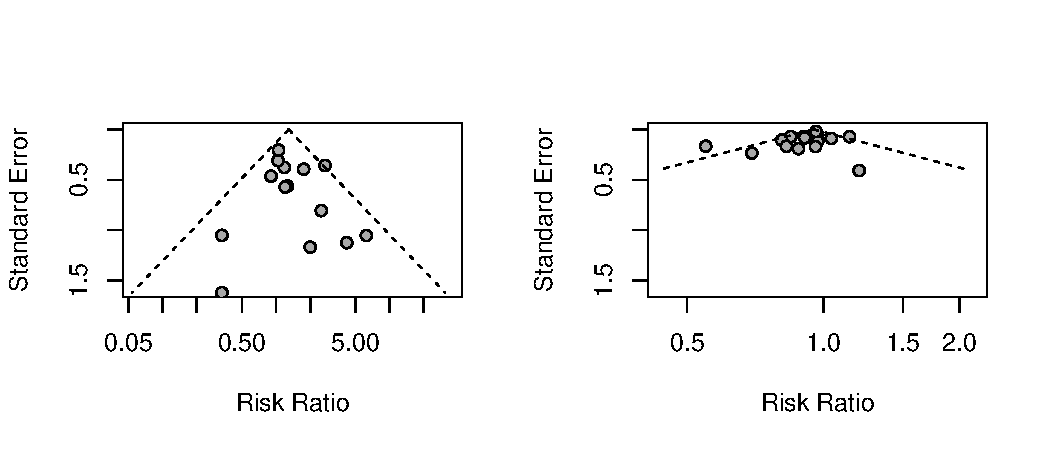
\includegraphics[width=\maxwidth]{figure/unnamed-chunk-1-1} 

\end{knitrout}
\caption{Funnel plots of two meta-analyses: On the left, the improvement in depression syndromes after application of tricyclic antidepressants is compared to placebo. The meta-analysis on the right measures the occurrence of intracranial haemoerrhage by CT after application of any anti-thrombolytic agent. All studies are RCT's.}
\label{small.study.effect.examples}
\end{figure}


We see that while the studies in the meta-analysis on the right rather accumulate on the right side, they seem to be more evenly distributed in the right triangle. From this, we would ultimately conclude that some sort of bias or heterogeneity is distorting the estimate of the overall treatment effect.\\
The Cochrane Organisation has specialized on systematic reviews of healthcare interventions. Researchers that write a systematic review collect data across studies, review them and try to provide up-to-date information about specific treatment efficacy \citep{cochrane.handbook}. By systematic literature review, they try to circumvent the issue of publication bias.
Earlier research however suggests that the efforts are only partially successful, and that there still is publication bias within the reviews (\citealp{Egger}, \citealp{Ioannidis2007}, \citealp{kicinsky}, \citealp{vanAert.2019}). In these publications, Cochrane systematic reviews is analysed with methods to detect publication bias, for example small study effect tests or Bayesian hierarchical selection models \citep{kicinsky}. They all find moderate to large evidence for publication bias in the database.\\

\section{Aim of the Study}
None of the research so far has estimated the amount and impact of publication bias on meta-analytical findings thoroughly and with the most suitable methods. Also, the results are ironically often presented in the form of dichotomous hypothesis tests, a practice that is partly responsible for publication bias.\\
The aim of this thesis was to use prevailed methods to detect publication bias, and make use of the full amount of data that the Cochrane Organisation provides. The research questions are: Are effects in meta-analyses \textit{larger} if their standard errors are small, and are there \textit{more} significant effects than expected? and How can this affect the combined treatment effects as commonly obtained by meta-analysis?. To answer these questions, methods to detect and adjust for publication bias in meta-analysis are applied on the data.\\
At the end, we will not only give an estimate of publication bias in the Cochrane Library but also show to what extent treatment effects are overestimated. The analyses are exploratory, but may generate new hypotheses and stimulate future directions for confirmatory research.




%%%%%%%%%%%%%%%%%%%%%%%%%%%%%%%%%%%%%%%%%%%%%%%%%%%%%%%%%%%%%%%%%%%%%


% LaTeX file for Chapter 02


\chapter{Methods} \label{ch:methods}
\section{Introduction and Notation}
The interventions are restricted to comparisons of two treatment groups by some measure of melioration or worsening of health. The difference in this measure between the groups is referred to as the treatment effect. Where it is not particularly mentioned, the term treatment effect refers to any effect measure such as log risk ratio, log hazard ratio, log rate ratio, Cohen's $d$ or standardized mean difference, Fisher's z transformed score.\\
Let us consider a meta-analysis with $n$ study treatment effects ($n > 1$, but typically small). A study is indexed by $i$, and it's treatment effect by  $\theta_i$. The observed treatment effect is $\hat{\theta}_i$. The pooled treatment effect of a meta-analysis will be denoted as $\theta_M$, and consequently, the observed pooled treatment effect as $\hat{\theta}_M$. Furthermore, each treatment effect is typically measured with some standard error $\se_i$ and an estimate of $\se_i$ is denoted as $\hat{\se}_i$. The $\hat{}$ sign thus indicates if it is an estimate.\\
For continuous outcomes, let $m_t$ be the mean of the treatment group, $m_c$ the mean of the control group, and equivalently $\textrm{sd}_t$ and $\textrm{sd}_c$ the corresponding standard deviations. 
In the case of binary outcomes, let $e_t$ be the count of events in the treatment arm $e_c$ the events in the control group. $n_t$ and $n_c$ are the total number of participants in the groups ($c$ for control and $t$ for treatment).%The observed counts in a study $i$ are referred to as $e_{t,i}$ and analogously $e_{c,i}$.

\section{Effect Measures and $p$\hspace{0.4mm}-values}
\subsection{Continuous Outcomes}
For given $(m_t, m_c), (\textrm{sd}_t, \textrm{sd}_c)$ and $(n_t, n_c)$, one can compute mean difference as well as a standardized mean difference (also known as Cohen's $d$) and the standard error thereof.

\begin{align}
\theta &= m_t - m_c & \se &= \sqrt{\textrm{sd}_t^2/n_t + \textrm{sd}_c^2/n_c}
\end{align}

Cohen's $d$ and its standard error $\se$ can similarly be obtained by

\begin{align}
d &= \frac{m_t - m_c}{\se} \label{eq:hedges.g} & \se &= \sqrt{\frac{(n_t - 1)\textrm{sd}_t^2 + (n_c - 1)\textrm{sd}_c^2}{n_t + n_c - 2}}
\end{align}

Both estimators take into account that the two groups might have unequal variances. \\ 
A  $p$\hspace{0.4mm}~-~value to test the null hypothesis that the mean between group is equal is commonly obtained with the Students $t$-test. The $t$ statistic is obtained, using $\se$ and $d$ from \eqref{eq:hedges.g}, by

\begin{align}
t &= d/(\se\sqrt{(1/n_t)+(1/n_c)}) \nonumber
\end{align}
and the  $p$\hspace{0.4mm}~-~value can be obtained with the cumulative Student's $t$-distribution $F$ with $n_t + n_c - 2$ degrees of freedom:

\begin{align}
p &= 2(1-F(\abs{t})) \nonumber
\end{align}

%The $t$-test is known to be reliable if combined sample size is small ($n_t + n_c < 30$), larger.

\subsection{Binary Outcomes}
Two commonly used effect measures for binary outcome data are risk ratios and odds ratios between treatment and control groups. 
The methods presented here can also be found, for example, in \cite[34]{Intro.meta}.
Let $\theta$ be the natural logarithm of the odds ratio. $\hat{\theta}$ and its variance $\hat{\se}^2$ can be obtained by computing

\begin{align}
\hat{\theta} &= \log(\frac{e_t\cdot(n_c - e_c)}{e_c\cdot(n_t - e_t)}) \nonumber \\
\hat{\se}^2 &= 1/e_t + 1/(n_t - e_t) + 1/e_c + 1/(n_c - e_c) \nonumber
\end{align}

Plugging in the observed counts will give the corresponding estimates. The logarithm of the risk ratio $\theta$ and its variance $\se^2$ is similarly defined as

\begin{align}
\hat{\theta} &= \log(\frac{e_t/n_t}{e_c/n_c}) \label{eq:risk.ratio} \\
\se^2&= 1/e_t - 1/n_t + 1/e_c - 1/n_c \label{eq:risk.ratio.variance}
\end{align}

Assuming binomial distribution of the events and using likelihood theory, one could show that the estimators are maximum likelihood estimators and that one can use the asymptotic normal distribution of the maximum likelihood estimator to calculate a  $p$\hspace{0.4mm}~-~value, \eg \cite[98]{held2014}. The approximation is only good if there are enough events and sample size is large enough.\\
Thus, with $\Phi$ as the cumulative standard normal distribution, we get
\begin{align}
p &= 2\cdot(1-\Phi(|\hat{\theta}/\hat{\se}|), \nonumber
\end{align}
a  $p$\hspace{0.4mm}~-~value for the corresponding estimate, which summarizes the evidence against $\hat{\theta}$ being zero (\ie the true risk/odds ratio being 1). \\
Odds ratios can be transformed to std. mean differences, which will be described in Section \ref{sec:transformation.effectsizes}.

\subsection{Time-to-Event Outcomes}
Usually, time-to-event data of two experimental groups can be compared by rate ratios. The normal approximations of the maximum likelihood estimators also works here when using the log rate ratio.
Time-to-event data with censoring has to be analyzed by special means. One frequently used method to take into account right-censoring is the Cox proportional hazards regression model \citep{Cox}. Because the method itself is not applied in this thesis, but only the resulting estimates of the parameters are used, the reader is referred to the extensive literature covering this topic (\eg \citealp{Surv}). \\
The so-called hazard ratio estimated by Cox regression is the ratio of the instantaneous risk of experiencing the event between two groups. Because it is a maximum likelihood estimator, one can again use its Wald test statistic to test for equal hazards. Let $\hat{\theta}$ be an estimate of the log hazard ratio and $\hat{\se}$ an estimate of the standard error of it. As before
\begin{align}
p &= 2\cdot(1-\Phi(|\hat{\theta}/\hat{\se}(\hat{\theta})|) \nonumber
\end{align}
will give a  $p$\hspace{0.4mm}~-~value for the evidence against the null hypothesis.



\section{Fixed and Random Effects Meta-Analysis} \label{sec:meta.analysis}
The fixed effects meta-analysis estimator of the pooled treatment effect is a mean of the single treatment effect estimators, weighted by their standard errors \citep{fixed.effects.rosenthal}. Let $w_i = 1/\se_i^2$ be the weights, and $\theta_M$ be the pooled estimator and $\se_M^2$ its variance. Then 

\begin{align}
\theta_M &= \frac{\sum_{i = 1}^n w_i \theta_i}{\sum_{i = 1}^n w_i} &
\se_M^2 &= \frac{1}{\sum_{i = 1}^n w_i} \label{eq:fixed.effects}
\end{align}

This estimator minimizes the variance between the effects. An estimate $\hat{\theta}_M$ can be obtained by plugging in the observed treatment effects and variances $\hat{\theta}_i$ and $\hat{\se}_i^2$. The underlying idea is that we assume $\theta_i \sim N(\theta_M, \se_i^2)$, $\theta_M$ being the true effect, all $\theta_i$ being distributed around an equal mean. \\
The random effects model \citep{whitehead} assumes instead that 
\begin{align}
\theta_i \sim N(\mu_i, \se_i^2) &&
\mu_i \sim N(\theta_M, \tau^2) \label{eq:random.effects} 
\end{align}

Marginally, we have $\theta_i$ being distributed around a common mean $\theta_M$ with additional variance $\tau^2$:

\begin{align}
\theta_i \given \mu_i \sim N(\theta_M, \se_i^2 + \tau^2) \nonumber %\label{eq:random.effects.marginal}
\end{align}

$\tau^2$ is often referred to as a population variance or between-study variance, whereas $\se_i^2$ can be interpreted as sampling error. The pooled treatment effect estimate $\theta_M$ of the random effects model and its variance is obtained by replacing the weights $w_i$ in equation \eqref{eq:fixed.effects} with $w_i = 1/(\se_i^2 + \tau^2)$.\\
The model is superior to the fixed effects model whenever the standard errors of the treatment effects alone are unlikely to fully account for the entire variability observed between studies. The method assigns larger weights to studies with larger standard errors.\\
The estimation of $\tau^2$ has been subject to some debate in the statistical literature. Oftentimes, the method of moment estimator of \citet{tau.estimator} is used. We use the measure of heterogeneity, $Q$, and divide by $C$ after having subtracted the degrees of freedom $n-1$:

\begin{align}
Q &= \sum_{i = 1}^n w_i(y_i - \theta_M)^2 & C &= \sum_{i = 1}^n w_i - \frac{\sum_{i = 1}^n w_i^2}{\sum_{i = 1}^n w_i} \label{eq:Q.heterogeneity} \\
\tau^2 &= \max\big(0, \frac{Q - (n-1)}{C}\big) \label{eq:Tau.definition}
\end{align}

The estimators have to be replaced by their estimates in order to get an estimate $\hat{\tau}^2$.\\
The Paule-Mandel estimator \citep{paulemandel} is considered to have better properties than the method of moments estimator (\eg \citealp{tau.estimator.evaluation}). Since we defined $w_i = 1/(\se_i^2 + \tau^2)$, it also holds that

\begin{align}
w_i \textrm{Var}(\theta_i) &= 1 & \textrm{Var}(\sqrt{w_i}\theta_i) = 1 \nonumber
\end{align}

For any $w_i$, the variance can be estimated and equated to its expected value:

\begin{align}
\se^2(w_i\theta_i) &= \frac{\sum_{i = 1}^n w_i(\theta_i - \theta_M)^2}{n-1} & \frac{\sum_{i = 1}^n w_i(\theta_i - \theta_M)^2}{n-1} = 1 \label{eq:paulemandel}
\end{align}

After estimating $\theta_M$ with equation \eqref{eq:fixed.effects}, the only problem remaining is to estimate $\tau^2$. $\hat{\tau}^2$ can be obtained through an iterative process, using a newly defined function

\begin{align}
F(\tau^2) &= \sum_{i = 1}^n w_i(\theta_i - \theta_M)^2 - (n-1) \nonumber
\end{align}

In view of equation \eqref{eq:paulemandel}, $\tau^2$ must be such that $F(\tau^2) = 0$. Then, we start with a arbitrary $\tau^2$ and repeatedly add a term $\tau_0^2$ to update $\tau^2$ until $F(\tau^2 + \tau_0^2)$ is close to zero (using $\tau^2 + \tau_0^2$ for $\hat{w}_i, \hat{\theta}_M$). Using a truncated Taylor series expansion, one can obtain the partial derivative after $\tau^2$, which is a reasonable choice for $\tau_0^2$. Using $\tau^2 + \tau_0^2$ for $\hat{w}_i, \hat{\theta}$, we can update $F(\tau^2)$ and check convergence to zero. \\
The estimation of $\tau^2$ is accompanied by uncertainty. A common procedure is to test if it is there is significant heterogeneity between the studies \cite[p. 109]{Intro.meta}. For this, $Q$ has to be computed as given in \eqref{eq:Q.heterogeneity}. It is assumed that $Q$ follows a central Chi-squared distribution with $n -1$ degrees of freedom under the null hypothesis of equally distributed effect sizes. Thus, the expected value of $Q$ is $n-1$, and the excess dispersion is $Q - n + 1$. The  $p$\hspace{0.4mm}~-~value against the null hypothesis of equally distributed effect sizes is $1 - F(Q)$, using $F$ as the cumulative distribution function of the Chi-squared distribution with d.f. = $n-1$. \\
$\tau^2$ is  is directly linked to the variability in the data. The $I^2$ statistic of excess/total dispersion can be used alternatively to assess the extent of additional variance to the variances of the primary study estimates. It is computed as

\begin{align}
I^2 &= \max\Big(0, 1 - \frac{n-1}{Q}\Big) \nonumber%\label{I2.proportion}
\end{align}

The statistic takes values between zero and one, and is easily interpretable. 0 is equal to 0\% excess dispersion and \eg 0.5 equal to 50\% additional between-study variance of the total variance of the estimates. \\
Importantly, all proposed methods above assume normally distributed effect sizes and proper estimates $\hat{\se}$ of the true standard error. This assumptions are not met for very small sample sizes and very few event counts. Alternatively, the Mantel-Haenszel method for risk and odds ratios (see \eg \citealp{mantel.haenszel}) could be used in the latter case. 




%%%%%%%%%%%%%%%%%%%%%%%%%%%%%%%%%%%%%%%%%%%%%%%%%%%%%%%%%%%%%%%%%%%%%%%%%%%%%%%%%%%%%%%%%%%%%%%%%%%%%%%%%%%%%%%%%%%%%%%%%%%%%%%%%%%%%%%%%%%%%%%%%%%%%%%%
%%%%%%%%%%%%%%%%%%%%%%%%%%%%%%%%%%%%%%%%%%%%%%%%%%%%%%%%%%%%%%%%%%%%%%%%%%%%%%%%%%%%%%%%%%%%%%%%%%%%%%%%%%%%%%%%%%%%%%%%%%%%%%%%%%%%%%%%%%%%%%%%%%%%%%%%
%%%%%%%%%%%%%%%%%%%%%%%%%%%%%%%%%%%%%%%%%%%%%%%%%%%%%%%%%%%%%%%%%%%%%%%%%%%%%%%%%%%%%%%%%%%%%%%%%%%%%%%%%%%%%%%%%%%%%%%%%%%%%%%%%%%%%%%%%%%%%%%%%%%%%%%%
%%%%%%%%%%%%%%%%%%%%%%%%%%%%%%%%%%%%%%%%%%%%%%%%%%%%%%%%%%%%%%%%%%%%%%%%%%%%%%%%%%%%%%%%%%%%%%%%%%%%%%%%%%%%%%%%%%%%%%%%%%%%%%%%%%%%%%%%%%%%%%%%%%%%%%%%
%%%%%%%%%%%%%%%%%%%%%%%%%%%%%%%%%%%%%%%%%%%%%%%%%%%%%%%%%%%%%%%%%%%%%%%%%%%%%%%%%%%%%%%%%%%%%%%%%%%%%%%%%%%%%%%%%%%%%%%%%%%%%%%%%%%%%%%%%%%%%%%%%%%%%%%%
%%%%%%%%%%%%%%%%%%%%%%%%%%%%%%%%%%%%%%%%%%%%%%%%%%%%%%%%%%%%%%%%%%%%%%%%%%%%%%%%%%%%%%%%%%%%%%%%%%%%%%%%%%%%%%%%%%%%%%%%%%%%%%%%%%%%%%%%%%%%%%%%%%%%%%%%

\section{Linear, Weighted and Linear Mixed Regression Models} \label{sec:regression}
First, the concept of simple linear regression is introduced \citep{fahrmeir2007}. In short, the model assumes a dependent variable $y$ to be a linear function of another explanatory variable $x$, with the residuals being distributed independently and identically and following a normal distribution:

\begin{align}
y &= \beta_0 + \beta_1 x + \epsilon, & \epsilon \sim N(0, \sigma^2) \label{eq:simple.regression}
\end{align}

$\epsilon$ is the residual noise term that becomes necessary when $n$ pairs $(x_i, y_i)$ are given and there is no exact solution. We look for the solution that minimizes the squared residuals, the least-squares solution. Formally,

\begin{align}
\operatorname*{argmin}_{\beta_0, \beta_1}\Big(\sum_{i = 1}^n y_i - \beta_0 - \beta_1 x_i\Big) \label{eq:least.squares}
\end{align}

Let $\mathbf{X}$ be a matrix with the explanatory variables $x$ and $\mathbf{y}$ a corresponding vector for all $y$:

\begin{equation*}
\mathbf{X} = 
\begin{bmatrix}
1 & x_{12} \\
1 & x_{22} \\
1 & x_{32} \\
\vdots & \vdots \\
1 & x_{n2} \\
\end{bmatrix} 
\qquad
\mathbf{y} = 
\begin{bmatrix}
y_1 \\
y_2 \\
y_3 \\
\vdots \\
y_n \\
\end{bmatrix}
\end{equation*}

\vspace{2mm}

Let $\mathbf{\beta} = (\beta_0, \beta_1)^\top$. It can be shown that 

\begin{align}
\hat{\mathbf{\beta}} &= (\mathbf{X}^\top \mathbf{X})^{-1} \mathbf{X}^\top \mathbf{y} \label{eq:regression.parameters}
\end{align}

Is an estimator of $\mathbf{\beta}$ that minimizes the squared residuals. Let $\hat{\mathbf{y}} = \mathbf{X}\hat{\mathbf{\beta}}$ and $\hat{\mathbf{r}} = \hat{\mathbf{y}} - \mathbf{y}$. The variance estimates $\hat{\sigma}^2$ and $\hat{\mathbf{s}}_\beta^2$ are

\begin{align}
\hat{\sigma}^2 &= \frac{1}{n-2}\mathbf{r}^\top \hat{\mathbf{r}} & \hat{\mathbf{s}}_\beta^2 &= \hat{\sigma}^2 (\mathbf{X}^\top \mathbf{X})^{-1} \label{eq:regression.variances}
\end{align}

If one plots the values of $y$ and $x$, the estimate $\hat{\beta}_0$ is the intercept and $\hat{\beta}_1$ the slope of the regression line. Furthermore, in the simple linear regression setting, $\hat{\beta}_0$ can also be obtained by:

\begin{align}
% \hat{\beta_1} &= \frac{\sum_{i = 1}^n (x_i - \bar{x})(y_i - \bar{y})}{\sum_{i = 1}^n (x_i - \bar{x})^2} &
\hat{\beta}_0 &= \bar{y} - \hat{\beta}_1 \bar{x} \nonumber
\end{align}

$\bar{x}$ and $\bar{y}$ denoting the sample means of the corresponding values $x_1, .., x_n$ and $y_1, ..., y_n$. Thus, $\hat{\beta}_0$ is also called the global mean.
To test whether there is evidence for the intercept $\beta_0$ to be unequal to some value $\beta_{H0}$, a $t$-test can be used. 

\begin{align}
p &= 2(1-F(\abs{(\beta_0 - \beta_{H0})/s_{\beta_0}})) \nonumber
\end{align}

where $F$ is the cumulative $t$ distribution with $n-2$ degrees of freedom. The  $p$\hspace{0.4mm}~-~value will give the evidence against the null hypothesis $\beta_0 = \beta_{H0}$. \\
The concept is extendable to weighted linear regression. Weighted linear regression may be used if the residuals $\mathbf{r}$ have unequal variances, which is equivalent to ascribe different precision to the observed $y$ (heteroscedasticity). The least squares equation \eqref{eq:least.squares} is extended as follows:

\begin{align}
\operatorname*{argmin}_{\beta_0, \beta_1}\Big(\sum_{i = 1}^n w_i(y_i - \beta_0 - \beta_1 x_i)\Big) \nonumber
\end{align}

with the positive weights $w_i$ penalizing large squared residuals for some $i$ more if $w_i$ is larger. \\
Let $\mathbf{W}$ be a $n \times n$ matrix with $\mathbf{W}_{ii} = w_i$, the weights on the diagonal and zeros on the off-diagonals. The estimates in \eqref{eq:regression.parameters} and \eqref{eq:regression.variances} can again be used if $\mathbf{X}$ is exchanged with $\mathbf{X}^\star =  \mathbf{W} \mathbf{X}$ and $\mathbf{y}$ with $\mathbf{y}^\star = \mathbf{W} \mathbf{y}$. \label{weighted.regression} \\
The introduction of group-specific random effects allows to analyze grouped or repeated measurements by linear regression. Let $j$ be the group index, $i$ the index of the single observation from the group $j$ and $x_i$ the $i^\textrm{th}$ row of $\mathbf{X}$, $(1, \mathbf{X}_{i2})$. Then the equation

\begin{align}
\mathbf{y}_i|U_j,\epsilon_{i} =  x_i\beta + U_j + \epsilon_{i} \label{eq:one.random.intercept}
\end{align}

gives the marginal distribution of $\mathbf{y}_i$ depending on $U{_j}$ and $\epsilon_i$. The random effects $U_j \sim N(0, \mathbf{G})$ and the residual error term $\epsilon_i \sim N(0, \tau^{2})$ are independent from each other. Let $\mathbf{y}_j$ be a vector of all observations of group $j$. The expectation $\mathbb{E}(\mathbf{y}_i)$ is still $x_i \beta$, but the covariance between the observations within a group $j$, is modeled as

\begin{align}
\Cov(\mathbf{y}_j) &= \mathbf{D}_j \mathbf{G} \mathbf{D}_j^\top + \tau^2 \mathbf{I}_{n_j} \label{eq:random.intercepts.covariance}
\end{align}

where $\D_j$ is in the case of the random intercept model a $n_j \times 1$ matrix of 1's, $\mathbf{G}$ is a scalar to be estimated and $\mathbf{I}_{n_j}$ is an $n_j \times n_j$ identity matrix. Thus, if $\mathbf{G} \neq 0$, the observations within a group will be uniformly correlated (uniform correlation between each observation). \\
Nested groups can be modeled by extending the design matrix $\mathbf{X}$ with an additional column of 1's and using according indices that specify the nesting structure.\\
An extension of the random intercepts model is the random slopes model, which allows for additional, group-specific slopes with respect to a explanatory variable $x$. It can be implemented by modifying \eqref{eq:one.random.intercept}. Let $\mathbf{U}_j$ be a two-dimensional random vector with a $2 \times 2$ covariance matrix $\mathbf{G}$. Again, we can specify the marginal distribution of a observation $i$ within a group $j$:

\begin{align}
\mathbf{y}_i|U_j,\epsilon_i =  x_i\beta + x_i \mathbf{U}_j + \epsilon_i \label{eq:one.random.intercept.and.slope}
\end{align}

$\mathbf{D}_j$ is a $n_i \times 2$ equal to all rows of observations of $j$ in $\mathbf{X}$. The covariance matrix $\mathbf{V_j}$ for group $j$ is defined as in equation \eqref{eq:random.intercepts.covariance}, using the new $\mathbf{D}_j$. Defining $\mathbf{x}_j$ as the matrix with all observations from group $j$ of $\mathbf{X}$, and equivalently the vector $\mathbf{y}_j$, $\hat{\beta}$ is obtained by computing

\begin{align}
\hat{\beta} &= \Big( \sum_{j = 1}^m \mathbf{x}_j^\top \hat{\mathbf{V}}_j^{-1} \mathbf{x}_j \Big)^{-1} \sum_{j = 1}^m \mathbf{x}_j^\top \hat{\mathbf{V}}_j^{-1} \mathbf{y}_j
\end{align}

with $m$ being the number of groups and $\hat{\mathbf{V}}_j$ being the estimated covariance, obtained by maximizing the log likelihood of the normal distribution, as $\mathbf{y}_j$ is distributed as

\begin{align}
\mathbf{y}_j \sim N(\mathbf{x}_j \beta, \mathbf{V}_j)
\end{align}

The matrices $\sum_{j = 1}^m \mathbf{x}_j^\top \hat{\mathbf{V}}_j^{-1} \mathbf{x}_j$ and $\hat{\mathbf{V}}_j$ are assumed to be positive definite  . The approximate covariance matrix of $\hat{\beta}$ is given by

\begin{align}
\hat{\Cov}(\hat{\beta}) &= \Big( \sum_{j = 1}^m \mathbf{x}_j^\top \hat{\mathbf{V}}_j^{-1} \mathbf{x}_j \Big)^{-1}
\end{align}

Weights can be introduced by replacing $\mathbf{I}_{n_j}$ in \eqref{eq:random.intercepts.covariance} with the previously introduced weight matrix $\mathbf{W}_j$. Hypothesis tests for $\beta = \beta_\textrm{H0}$ can be made using the Wald method. \\
It is necessary to check the model assumptions after fitting a linear regression. For this purpose, fitted values can be plotted against standardized residuals. If the standardized residuals are not dispersed evenly around zero for any size of fitted values, the assumption of the residuals being independently and equally distributed around zero is violated and estimates are biased. \\










\section{Publication Bias Assessment}
The tests that will be presented on the following pages are a common way to detect publication bias. A frequently used method to test and adjust for publication bias, which goes under the name of trim-and-fill \citep{trimfill} is not discussed because of its disadvantageous properties (see \eg \citealp{Moreno.2009}).\\

\subsection{Begg and Mazumdar: Rank Correlation Test} \label{sec:Begg}
\citealp{begg.ties} proposed a rank based test to test the null hypothesis of no correlation between effect size and variance.
A standardized effect size $\theta_i^\star$ can be computed as in \eqref{eq:begg.stand.eff}. $\se_i^{2\star}$ is the variance of $\theta_i - \theta_M$ as defined in \eqref{eq:begg.stand.var} and $\theta_M$ is the fixed effects pooled treatment effect (\eqref{eq:fixed.effects}. 

\begin{align}
\theta_i^\star &= (\theta_i - \theta_M)/\se_i^{2\star} \label{eq:begg.stand.eff}  \\
\se_i^{2\star} &= \se_i^2 - 1/\sum_{i = 1}^n\frac{1}{\se_i^2} \label{eq:begg.stand.var} 
\end{align}

A rank correlation test based on Kendall's tau is then used. First, the pairs are ordered after their ranks based on $\se^{2\star}$. Then, for each $\se^{2\star}$ rank, the corresponding ranks based on $\theta^{2\star}$ that are larger are counted and summed up to $u$. The number of ranks based on $\theta^{2\star}$ that are in contrary, smaller, are counted and summed up to $l$. Then the normalized test statistic $Z$ is given as

\begin{align}
Z &= (u - l)/\sqrt{n(n-1)(2n + 5)/18} \nonumber
\end{align}

Thus, large number of concordant pairs will reflect in large $\hat{u}$ and small $\hat{l}$ and thus lead to a large $\hat{Z}$. A two-sided  $p$\hspace{0.4mm}~-~value is obtained using the standard normal distribution $\Phi$:
\begin{align}
p &= 2\cdot(1-\Phi(\abs{Z})) \nonumber
\end{align}

A one-sided test for positive correlation is obtained by computing $1-\Phi(Z)$ instead.
The changes that have to be made in the case of ties are small and can be found in \cite[p. 410]{begg.ties}.


\subsection{Egger's Test: Weighted Linear Regression Test} \label{sec:Egger}
Linear regression can be used to test dependency of effect sizes on study sizes. The simplest application was introduced by \citet{Egger}.
Let $\theta/\se$ be the dependent variable $y$ and $1/\se$ the explanatory variable $x$. If plotted, this corresponds to a radial or Galbraith plot \citep{galbraith}. The linear regression equation as introduced before in \eqref{eq:simple.regression} can be written in two ways:

\begin{align}
\theta/\se &= \beta_0 + \beta_1/\se + \epsilon, & \epsilon \sim N(0, \sigma^2) \label{eq:radial.plot} 
\end{align}

Equation \eqref{eq:radial.plot} is often provided due to the correspondence to the radial plot. However, it is equivalent to

\begin{align}
\theta &= \beta_0 + \beta_1 \se + \epsilon, & \epsilon \sim N(0, w^{-2}\sigma^2) \label{eq:egger.plot}
\end{align}

with weights $w = 1/\se^2$. Thus testing $\beta_0$ of \eqref{eq:radial.plot} or $\beta_1$ of \eqref{eq:egger.plot} is equivalent. The corresponding  $p$\hspace{0.4mm}~-~value is then used as evidence for a small study effect. Plugging in  $\theta_i/\se_i, 1/\se_i$ as $y_i, x_i$ into equations \eqref{eq:regression.parameters} and \eqref{eq:regression.variances} will give the estimates for $\hat{\beta}_0, \hat{\beta}_1,\hat{\se}_{\beta_0}$ and $\hat{\se}_{\beta_1}$.

% \begin{align}
% \hat{\beta_1} &= \frac{\sum_{i = 1}^n (\varphi_i - \bar{\varphi})(\theta^\star_i - \bar{\theta}^\star)}{\sum_{i = 1}^n (\varphi_i - \bar{\varphi})^2} &
% \hat{\beta}_0 &= \bar{\theta}^\star - \hat{\beta}_1 \bar{\varphi} \nonumber
% \end{align}


\subsection{Thompson and Sharp's Test: Weighted Linear Regression Random Effects Test} \label{sec:Thompson}
A method proposed in \citet{thompson.sharp} allows for between study variance $\tau^2$, as introduced before in section \ref{sec:meta.analysis}. It extends the previously seen linear regression approach with $x = 1/\se$ and $y = \theta/\se$ by introducing new weights. The effect size $\theta_i$ is assumed to be distributed as

\begin{align}
\theta_i \sim N(\beta_0 + \beta_1 \se_i, \se_i^2 + \tau^2) \label{t.sharp.regression}
\end{align}

$\tau^2$ is estimated as in equation \eqref{eq:Tau.definition} (method of moments). %or \eqref{eq:paule.mandel}. 
The weights are set as $w_i = 1/\sqrt{\se_i^2 + \tau^2})$. After adjusting for the weights as described in \ref{weighted.regression}, we can proceed analogous to Egger's test. The  $p$\hspace{0.4mm}~-~value for $\beta_{0} \neq 0$ reflects the evidence for a small study effect.


\subsection{Peters Test: Weighted Linear Regression Test} \label{sec:Peter}
When the outcome is dichotomous, effect sizes and variances of effect size are correlated, which can readily be seen in \eqref{eq:risk.ratio} and \eqref{eq:risk.ratio.variance} (see also \cite[p. 120]{meta.w.R}). A small number of event counts in one or group will inflate the variance and the effect size. Consequently, the tests above will tend to reject the null-hypothesis too often, \ie report false positives.\\ 
Instead of taking the standard error $\se$ as explanatory variable $x$ as in Egger's test, the inverse of the total sample size is used. Additionally, the variances $\se_i^2$ are used as weights. Thus, the subsequent test procedure is identical to Egger's test. Peters test is a a small modification of Macaskill's test where the explanatory variable is the sample size instead of its inverse. \\
The method will give less false positives than Egger's test, but will be more imprecise, because total sample size is not a very good approximation for statistical power (the overall rate of events in both groups plays an important role as well).



\subsection{Harbord's Test: Score based Test} \label{sec:Harbord}
A rank based alternative to Peters test for binary outcomes is Harbord's test \citep{Harbord}.
It uses a different treatment effect and variance estimate: the score $\varphi$ of the log-likelihood, evaluated as log odds ratio $\theta_\textrm{H0} = 0$ and its inverse Fisher information $s^2$. Formally,

\begin{align}
\varphi &= e_t - (e_t - e_c)(e_t + (n_t - e_t))/(n_t + n_c) \label{harbord.score} \\
 s^2 &= \frac{(e_t + e_c)(e_t + (n_t - e_t))(e_c + (n_c - e_c))((n_t - e_t) + (n_c - e_c))}{(n_t + n_c)^2(n_t + n_c - 1)} \label{harbord.variance}
\end{align}

It can be shown that they are both good approximations of the log odds ratio and its variance if the real $\theta$ is not too far from zero. The standardized estimator $\varphi_i/\se_i^2$ is also known as Peto odds ratio. The obtained scores and variances can be used in Egger's test as treatment effects and variances.


\subsection{Schwarzer's Test: Rank Correlation Test} \label{sec:Schwarzer}
\citealp{Schwarzer} developed a test for the correlation between the event counts in the treatment group and the expected event counts $E_t - \mathbb{E}(E_t)$. When the marginals in a two-by-two table and the log odds ratio are fixed, it can be shown that $E_t$ follows a non-central hypergeometric distribution. Using the Mantel-Haenszel log odds ratio and the marginal total parameters, the variance and the expectation of $E_t$ is calculated. The inverse of the variance $\se(E_t)^2$ and the standardized event count

\begin{align}
(e_t - \mathbb{E}(E_t))/\sqrt(\se_i^2)
\end{align}

are then used as before in Begg and Mazumdar's test.

\subsection{R\"ucker's Test: Using the Variance Stabilizing Transformation for Binomial Random Variables} \label{sec:Rucker}
The correlation between variance and effect size of dichotomous outcome measures can be abolished by the variance stabilizing transformation for binomial random variables. We use that the arcsine function is the variance stabilizing transformation for a proportion. Let

\begin{align}
\theta_i &= \arcsin{e_t/n_t} - \arcsin{e_c/n_c} \nonumber &
\se_i^2 &= 1/4n_t + 1/4n_c \nonumber
\end{align}

Then one can optionally apply Begg and Mazumdar's rank correlation test or Thompson and Sharp's test using the newly obtained estimates.


\subsection{Excess Significance Test} \label{sec:excess.significance}
Publication bias does not need to be accompanied by small study effects. In the absence of any treatment effect, significant effects could be included in a meta-analysis on both directions of treatment effects (\ie large \textit{and} small effects) are published. Also, the afore-mentioned methods do not use statistical significance directly to investigate publication bias. Thus, a different test is introduced. \\
\citealp{excess.significance} developed an exploratory test to detect if the proportion of significant findings is larger than expected. 
%Note that significance is here defined as one-sided significance, with the direction of the test being the same for each study. \\
We assume that the effects are equally distributed around a true mean effect $\theta_M$, which can be estimated by fixed effects meta-Analysis \eqref{eq:fixed.effects}. Let $O$ be the number of significant study results out of $n$ studies and $\alpha$ the significance threshold. Corresponding to the study effect $\theta_i$, we can specify the power $1 - \beta_i$, the probability to be accepting a true result. Let $z_{\alpha,i}$ be the $1-\alpha$ quantile of a normal distribution with standard error $\hat{\se}_i$. The power of study $i$ can be estimated as:

\begin{align}
1 - \hat{\beta}_i &= F(z_\alpha) 
\end{align}

with $F$ being the cumulative normal distribution with mean $\hat{\theta}_M$ and standard deviation $\hat{\se}_i$. \\
If we assume no bias in $\theta_i$ and $\theta_M$, the expected number of significant study results is then just

\begin{align}
E &= \sum_{i = 1}^n (1 - \beta_i) \nonumber
\end{align}

$E$ can then be compared to $O$ by constructing a test statistic $\chi$:

\begin{align}
\chi  &= \bigg( \frac{(O - E)^2}{E} + \frac{(O - E)^2}{n - E}\bigg) \nonumber
\end{align}

and consecutively, calculating a $p$\hspace{0.4mm}~-~value for the evidence against the null-hypothesis of $O = E$ with a $\chi^2$ distribution with one degree of freedom. Alternatively, one can also use a binomial test, which is encouraged when $n$ and $O$ is small. We will get a one sided $p$\hspace{0.4mm}~-value for excess significance, $\P(X \geq O)$, by computing

\begin{align}
p &= \sum_{i = O}^n\Big({n \choose i} p^i (1-p)^{n - i}\Big)
\end{align}

with $p = E/n$ and $X$ being a binomial random variable with probability $p$. 





%%%%%%%%%%%%%%%%%%%%%%%%%%%%%%%%%%%%%%%%%%%%%%%%%%%%%%%%%%%%%%%%%%%%%%%%%%%%%%%%%%%%%%%%%%%%%%%%%%%%%%%%%%%%%%%%%%%%%%%%%%%%%%%%%%%%%%%%%%%%%%%%%%%%%%%%
%%%%%%%%%%%%%%%%%%%%%%%%%%%%%%%%%%%%%%%%%%%%%%%%%%%%%%%%%%%%%%%%%%%%%%%%%%%%%%%%%%%%%%%%%%%%%%%%%%%%%%%%%%%%%%%%%%%%%%%%%%%%%%%%%%%%%%%%%%%%%%%%%%%%%%%%
%%%%%%%%%%%%%%%%%%%%%%%%%%%%%%%%%%%%%%%%%%%%%%%%%%%%%%%%%%%%%%%%%%%%%%%%%%%%%%%%%%%%%%%%%%%%%%%%%%%%%%%%%%%%%%%%%%%%%%%%%%%%%%%%%%%%%%%%%%%%%%%%%%%%%%%%
%%%%%%%%%%%%%%%%%%%%%%%%%%%%%%%%%%%%%%%%%%%%%%%%%%%%%%%%%%%%%%%%%%%%%%%%%%%%%%%%%%%%%%%%%%%%%%%%%%%%%%%%%%%%%%%%%%%%%%%%%%%%%%%%%%%%%%%%%%%%%%%%%%%%%%%%
%%%%%%%%%%%%%%%%%%%%%%%%%%%%%%%%%%%%%%%%%%%%%%%%%%%%%%%%%%%%%%%%%%%%%%%%%%%%%%%%%%%%%%%%%%%%%%%%%%%%%%%%%%%%%%%%%%%%%%%%%%%%%%%%%%%%%%%%%%%%%%%%%%%%%%%%
%%%%%%%%%%%%%%%%%%%%%%%%%%%%%%%%%%%%%%%%%%%%%%%%%%%%%%%%%%%%%%%%%%%%%%%%%%%%%%%%%%%%%%%%%%%%%%%%%%%%%%%%%%%%%%%%%%%%%%%%%%%%%%%%%%%%%%%%%%%%%%%%%%%%%%%%






\section{Publication Bias Adjustment}
There are different approaches to correct for small study effects and publication bias. They can mainly be distinguished by their underlying methods: regression based approaches aim to regress the effect to a study with infinite precision (\ie very small standard error) or to a summary effect, corrected for publication bias. Selection models are used for a sensitivity analysis, where the selection parameters are assumed to be fixed. 

\subsection{Adjustment by Regression} \label{sec:regression.adjustment}
In \citet{limitmeta.2} and \citet{limitmeta}, a random effects model is proposed to obtain unbiased treatment effect estimates. Similarly to regression based tests for small study effects, we have

\begin{align}
\theta_i & = \beta_0 + \beta_1\sqrt{\se_i^2 + \tau^2} + \epsilon_i\sqrt{v_i + \tau^2}, \label{eq:limitmeta.regression} \\
\epsilon_i &\stackrel{\textrm{iid}}{\sim} N(0,1)
\end{align}

The only difference between Thompson and Sharp's variant and this method is that $x = \sqrt{\se^2 + \tau^2}$ is used instead of $x = \sqrt{\se^2}$. $\beta_{1}$ is the bias parameter and can be interpreted as the bias introduced by small study effects, as illustrated in the following equations:

\begin{align}
\mathbb{E}\big((\theta_i - \beta_0)/\sqrt{\se_i^2}\big) \rightarrow \beta_1 \textrm{ if } \se_i \rightarrow \infty \nonumber \\ %\label{limitmeta.infinitesample} \\
\mathbb{E}(\theta_i) \rightarrow \beta_0 + \beta_1 \tau \textrm{if} \se_i \rightarrow 0 \nonumber
\end{align}

After estimating $\tau^2$, one can estimate $\beta_{0}$ and $\beta_{1}$ as seen before in the simple linear regression framework.There are two possible estimates at hand:
\begin{itemize}
\item $\beta_0$ the treatment effect without any influence of study precision with standard error $\se_{\beta_0}$
\item $\beta_0 + \beta_1 \tau$ the treatment effect of a hypothetical study with infinite precision, corresponding standard error $\se = \se_{\beta_0} + \se_{\beta_1}$
\end{itemize}

Simulations in \citet{limitmeta} suggested that the latter estimate is slightly superior to the former, because it showed a smaller mean-squared error in simulation studies \citet{limitmeta.2}. From the formulas above, it becomes clear that is has a larger standard error. The results of the simulation furthermore emphasize that adjustment is more reliable when effects of publication bias are strong within a meta-analysis. When no publication bias affects the meta-analysis, and event rates are low, the method provided biased estimates and the mean squared error was large. The coverage of the confidence intervals was always larger or equal to meta-analysis. It outperforms or is equal to classical meta-analysis estimates with respect to coverage, mean squared error and bias if there is publication bias, especially if event rates in the control group are small. 



\subsection{Copas Selection Model} \label{sec:copas}

A method proposed in \cite{Copas1,Copas2,Copas3} assumes that study results are selected based on the specific properties of their effect sizes and variances. \\
Let $\theta_i$ be the effect size estimate of study $i$. Then 

\begin{align}
\theta_i &\sim N(\mu_i, \sigma_i^2) &
\mu_i \sim N(\theta, \tau^2) \label{eq:population.model}
\end{align}

which is identical to the random-effects meta-analysis setting. $\theta$ is the population mean effect, $\sigma_i^2$ the within study variance and $\tau^2$ the between study variance. This is termed the \textit{population model}. \\
The \textit{selection model} is defined as follows. Suppose a selection of studies with reported %($\neq$ estimated) 
standard errors $\se$ (possibly different from $\sigma$). Only a proportion of the selection will be published, with the parameter $a$ defining the overall proportion of published studies and $b$ (assumed to be positive) defining how fast this proportion increases with $\se$ becoming smaller. Formally, the probability of selection given a reported standard error $\se$ is defined as

\begin{align}
P(\textrm{select}\given \se) &= \Phi(a + b/\se) \nonumber %\label{copas.selection1}
\end{align}

The equation can be rewritten as 

\begin{align}
z = a + b/\se + \delta \nonumber %\label{copas.selection2}
\end{align}

with $\delta \sim N(0,1)$. $z$ is interpreted as the \textit{propensity for selection}. It is defined that the sign of $z$ must be positive in order for the study to be selected.
$a$ is some kind of global selection rate for each study and $b$ decides about the decline of selection probability with increasing $\se$.\\
So far, we have, for a study $i$

\begin{align}
\theta_i = \mu_i + \sigma_i\epsilon_i \nonumber \\ 
\mu_i \sim N(\theta, \tau^2) \nonumber \\
z_i = a + b/\se_i + \delta_i \nonumber
\end{align}

where $(\epsilon_i, \delta_i)$ are standard normal residuals. The two models are coupled by introducing a correlation $\rho = cor(\theta_i, z_i)$ by defining $(\epsilon_i, \delta_i)$ as bivariate standard normals. It follows that,
%Every given study $i$ in the meta-analysis has $z_i > 0$. 
if $\rho_i$ is unequal to zero and positive and $z_i > 0$, then the estimate of a study $i$ that is selected is likely to have positive $\delta_i$ and thus positive $\epsilon_i$, such that the true mean $\mu$ is likely to be overestimated. \\
Let $u_i = a + b/\se_i$, $\lambda(u_i)$ the Mill's ratio $\phi(u_i)/\Phi(u_i)$ ($\phi$ is the standard normal density function and $\Phi$ the cdf) and $\tilde{\rho_i} = \sigma/\sqrt(\tau^2 + \sigma_i^2) \rho_i$. The probability of a study being selected, given $\se_i$ and $\theta_i$, is

\begin{align}
P(\textrm{select} \given \se_i, \theta_i) = %P(a,b,s,y) = 
\Phi\bigg(\frac{u_i + \tilde{\rho_i}((\theta_i - \mu)/\sqrt(\tau^2 + \sigma_i^2))}{\sqrt{1 - \tilde{\rho_i^2}}}\bigg) \nonumber
\end{align}

Which shows that larger $\se_i$ and $\theta_i$ lead to a larger selection probability. It can also be shown that the expected value 

\begin{align}
\mathbb{E}(\theta_i \given \se_i, \textrm{select}) = \mu + \rho_i\sigma_i\lambda(u_i) \label{eq:copas.expectation}
\end{align}

increases for larger $\sigma$.\\
A likelihood for $\theta_i$, conditional on $z>0$ can be formulated to estimate the parameters of the model. $a$ and $b$ are not estimated because the number of missing studies and their effect sizes is not known. Instead, fixed values for $a$ and $b$ have to be imputed.
The nuisance parameter $\sigma_i$ can be estimated, as

\begin{align}
\textrm{Var}(\theta_i\given \se_i, z_i > 0) = \sigma_i^2 (1 - c_i^2\rho_i^2) \nonumber
\end{align}

with $c^2 = \lambda(u_i)(u_i + \lambda(u_i))$. Thus we can replace $\sigma_i^2$ by $\hat{\sigma}_i^2 = \frac{1}{1-c_i^2\rho_i^2}$. \\ 
With equation \eqref{eq:copas.expectation}, one can obtain fitted values of $\theta_i$ based on $\se_i$ and fixed $a$ and $b$. For two different pairs $(a,b)$, $(a^\star, b^\star)$,

\begin{align}
\mathbb{E}(\theta_i\given z_i > 0, a^\star, b^\star) - \mathbb{E}(\theta_i\given z_i > 0, a, b) \approx c^\star + \rho(\lambda(a^\star) - \lambda(a))\se_i \nonumber
\end{align}

Local departures of two fitted values of $\theta_i$ can be approximated by adding a linear term in $\se_i$ to the expectation of $\theta_i$. Thus, to test a single pair $(a,b)$ (chosen such that $\rho \geq 0$), it is sufficient to test $\beta \neq 0$ in

\begin{align}
\theta_i &= \theta + \beta \se_i + \sigma_i \epsilon_i \nonumber
\end{align}

If $\beta \neq 0$, there is still bias in the fitted values. To test a pair $(a,b)$ against the scenario with no selection, we set $a^\star = \infty$ (or $\rho = 0$) and $b^\star = 0$. A likelihood ratio test will give a test statistic to test against $H0 =$ no selection ($\beta \neq 0$):

\begin{align}
\chi^2 &= 2\cdot(\operatorname*{max1}_{\theta, \tau, \beta}\tilde{L}(\theta, \tau, \beta) - \operatorname*{max}_{\theta, \tau}\tilde{L}(\theta, \tau, 0)) \label{eq:copas.small.study}
\end{align}

with 
\begin{align}
\tilde{L}(\theta, \tau, \beta) = -\frac{1}{2}\sum_{i = 1}^n[\log(\tau^2 + \sigma_i^2) + \frac{(\theta_i - \theta - \beta \se_i)^2}{(\tau^2 + \sigma_i^2)}] \nonumber
\end{align}

$\chi^2$ can be used with a $\chi^2$ distribution with one degree of freedom to obtain a $p$\hspace{0.4mm}~-~value. Note that the test is very similar to Egger's small study effect test when $\tau^2 = 0$.\\
In practice one can observe how $\theta$ and it's confidence intervals change dependent on the underlying selection process, and how the choice of the parameters affect the evidence for remaining publication bias (selection). \citet{limitmeta} used the method in a simulation for inference purposes, and have implemented it in the \citet{meta.package}. However, in the simulations, the method was outperformed by the regression adjustment method when publication bias was present. Especially when event rates in the control group were small and publication bias was strong, bias, mean squared error and coverage was substantially worse. Other authors argue that selection models should in general not be used for inference (\eg \citealp{selection.assessment}).\\
The procedure in \citet{limitmeta} is the following: A range of values of $(a,b)$ are applied, and the test for residual small study effect as described in equation \eqref{eq:copas.small.study} is applied. If all obtained  $p$\hspace{0.4mm}~-~values from the test are above a threshold 0.1, this is interpreted as no evidence, and no need for adjustment, and the standard, classical random effects meta-analysis is retained. If none of the  $p$\hspace{0.4mm}~-~values is above the threshold, a wider range of values for $(a,b)$ is used. When some  $p$\hspace{0.4mm}~-~values are above, and some below the threshold, the pair $(a,b)$ with the smallest number of missing studies is retained (that is, the pair of $a$ and $b$ that implies the fewest publication bias is chosen).\\
Currently, there is no test to detect miss-specifications in the model itself and the authors themselves have argued that a non-parametric test of the residuals would lack power.



\section{Transformation between Effect Measures} \label{sec:transformation.effectsizes}
Assuming that binary outcomes result from a dichotomization of originally continuous random variables, binary outcome measure can be transformed into continuous outcome measures. Here, the logistic distribution is used to achieve the transformation from a typical binary effect measures to a std. mean difference \cite[47]{Intro.meta}.\\
Let $\theta$ be a log odds ratio and $\se$ it's standard error. The std. mean difference $d$ and it's variance $\se_d^2$ can be obtained as

\begin{align}
d &= \theta \frac{\sqrt{3}}{\pi} & \se_d^2 =  \se^2\frac{\sqrt{3}}{\pi} \nonumber
\end{align}

The factor $\frac{\pi}{\sqrt{3}} = 1.81$ is the standard deviation of the logistic distribution $L(\mu, \eta)$ with scale parameter $\eta = 1$, so we just divide the log odds ratio and it's variance through the standard deviation. The approximation works only well if $e_t$ and $e_c$ are not very small, especially in the case of $\se_d^2$. \\
The Pearson's correlation coefficient can be attained by the formulas (\citealp{olkin1985dtor}, \cite[48]{Intro.meta})

\begin{align}
r &= \frac{d}{\sqrt{d^2 + a}} & a = (n_c + n_t)^2 / n_c n_t \nonumber
\end{align}

where $a$ is a correction factor if $n_t \neq n_c$. The variance of $r$, $\se_r^2$ is computed by

\begin{align}
\se_r^2 &= \frac{a^2 \se_d^2}{(d^2 + a)^3} \nonumber
\end{align}

Finally, we can get to a fisher's z-transformed correlation $z$ and it's variance $\se_z^2$ by using
\begin{align}
% z &= 0.5 \ln\big(\frac{1 + r}{1 - r}\big) & \nonumber
z &= \arctan(r) & \nonumber
\se_z^2 &= \frac{1}{n-3}
\end{align}

%%%%%%%%%%%%%%%%%%%%%%%%%%%%%%%%%%%%%%%%%%%%%%%%%%%%%%%%%%%%%%%%%%%%%%


% LaTeX file for Chapter 03










\chapter{The Cochrane Dataset} \label{ch:dataset}


\section{Cochrane Systematic Reviews}
Cochrane has specialized on systematic reviews in clinical science. Certain knowledge of standards and principles of the organization may help to understand the dataset. The following information stems from the Cochrane Handbook for Systematic Reviews \citep{cochrane.handbook}. \\
The definition of a systematic review is that it ``attempts to collate all empirical evidence that fits pre-specified eligibility criteria in order to answer a specific research question.'' Thus, the ``key properties of a review are'':

\begin{itemize}
\item``a clearly stated set of objectives with pre-defined eligibility criteria for studies''
\item ``an explicit, reproducible methodology''
\item ``a systematic search that attempts to identify all studies that would meet the eligibility criteria''
\item ``an assessment of the validity of the findings of the included studies, for example through the assessment of risk of bias''
\end{itemize}

At the end of a systematic review, ``a systematic presentation, and synthesis, of the characteristics and findings of the included studies'' is done. \\
53 Cochrane Review Groups prepare and maintain the reviews within specific areas of health care. A group consists of ``researchers, healthcare professionals and people using healthcare services (consumers)''. \\
The groups are supported by Method Groups, Centers and Fields. The Cochrane Method Groups aim to discuss and consult the groups in methodological questions concerning review preparation. The Centers play a main role in training and support of the Groups. The Fields are responsible for broad medical research areas and follow priorities in those areas by advice and control of the groups. \\
The first step in a review is writing a protocol, specifying the research question, the methods to be used in literature search and analysis and the eligibility criteria of the study. Changes in protocols are possible but have to be documented and the protocol is published in advance of the publication of the full review. The choices of methodology as well as the changes should not be made ``on the basis of how they affect the outcome of the research study''. \\
In order to avoid potential conflicts of interests, there is a code of conduct that all entities of Cochrane have to agree on: conflicts of interest must be disclosed and possibly be forwarded to the Cochrane Center, and participation of review authors in the studies used have to be acknowledged. Additionally, a Steering Group publishes a report of potential conflicts of interests based on information about external funding of Cochrane Groups. \\
In order for keeping the reviews up-to-date, they are revised in a two-year circle with exceptions. In addition to inclusion of new evidence in a field, the revision and maintenance process may as well includes change in analysis methods. This can reflect some advance in clinical science as for example new information about important subgroups, as well as new methods for conducting a Cochrane review. However, there are no clear guidelines and the Cochrane Groups are free in the rate and extent of up-dating their reviews.

\subsection{Methods for Cochrane Reviews}
A research question defines the following points: ``the types of population (participants), types of interventions (and comparisons), and the types of outcomes that are of interest''. From the research question, usually the eligibility criteria follow. Usually, outcomes are not part of eligibility criteria, except for special cases such as adverse effect reviews. \\
The type of study is an important eligibility criterium. Cochrane focuses ``primarily on randomized controlled trials'', and also, the methods of study identification in literature search are focused on randomized trials. Furthermore, study characteristics such as blinding of study operators with respect to treatment and cluster-randomizing might be additional eligibility criteria which have to be chosen by the review authors. \\
After having specified the eligibility criteria, studies have to be collected. The central idea of systematic reviews, and also meta-analyses, is that the collected studies are a random sample of a population of studies, i.e. that they are representative and can be used to assess population properties. Therefore, the search process is crucial, as a selective search result may impose bias on the sample of studies available, making it a non-random sample. For this purpose, the Cochrane Groups are advised to go beyond MEDLINE, because a search restricted to it has been shown to deliver only 30\% to 80\% of available studies. ``Time and budget restraints require the review author to balance the thoroughness of the search with efficiency in use of time and funds and the best way of achieving this balance is to be aware of, and try to minimize, the biases such as publication bias and language bias that can result from restricting searches in different ways.'' It is important to note that not only studies, but also study reports are occasionally used in the reviews, as they may provide useful information. \\
There are different sources that are being used to search for studies. 
\begin{itemize}
\item The Cochrane Central Register of Controlled Trials is a source of reports of controlled trials. ``As of January 2008 (Issue 1, 2008), CENTRAL contains nearly 530,000 citations to reports of trials and other studies potentially eligible for inclusion in Cochrane reviews, of which 310,000 trial reports are from MEDLINE, 50,000 additional trial reports are from EMBASE and the remaining 170,000 are from other sources such as other databases and handsearching.'' It includes citations published in many languages, citations only available in conference proceedings, citations from trials registers and trials results registers.
\item MEDLINE includes over 16 million references to journal articles. 5,200 journals publishing in 27 languages are indexed for MEDLINE. PubMed gives access to a free version of MEDLINE with up-to-date citations. NLM gateway such as the Health Services Research Project, Meeting Abstracts and TOXLINE Subset for toxicology citations allows for search in both databases together with additional data from the US National Library of Medicine.
\item EMBASE. 4,800 journals publishing in 30 languages are indexed in EMBASE, which includes more than 11 million records from 1974 onward. EMBASE.com also includes 7 million unique records from MEDLINE (1966 up to date) together with its own records. Additionally, EMBASE Classic allows access to digitized records from 1947 to 1973. EMBASE and MEDLINE each have around 1,800 journals not indexed in any other database.
\item Regional or national and subject specific databases can additionally be consulted and often provide important information. Financial considerations may limit the use of such databases.
\item General search engines such as Google Scholar, Intute and Turning Research into Practice (TRIP) database can be used.
\item Citation Indexes. The database lists articles published in around 6,000 journals with articles in which they have been cited and is available online as SciSearch. This form of search is known as cited reference searching.
\item Dissertation sources. Dissertations are often listed in MEDLINE or EMBASE but one is advised to also search in specific dissertation sources.
\item Grey Literature Databases. Approximately 10\% of the results in the Cochrane Library stems from conference abstracts and other grey literature. The Institute for Scientific and Technical Information in France provides access to entries of the previously closed System for Information on Grey Literature database of the European Association for Grey Literature Exploitation. Another source is the Healthcare Management Information Consortium (HMIC) database containing records from the Library and Information Services department of the Department of Health (DH) in England and the King's Fund Information and Library Service. The National Technical Information Service (NTIS) gives access to the results of US and non-US government-sponsored research, as well as technical report for most published results. References from newsletters, magazines and technical and annual reports in behavioral science, psychology and health are provided in the PsycEXTRA database which is linked to PsycINFO database.
\end{itemize}


\section{Structure and Variables}
The dataset consists of 6,354 systematic reviews from the Cochrane Library with 70,662 studies and 744,720 results. A result of a study can be a primary or secondary or safety outcome, thus studies can contribute multiple results. The studies too a very large extent randomized and investigate the effects of healthcare and medical interventions and treatments. The reference to the treatment may be a placebo control or a different intervention or treatment. A result can not only be about efficacy of the treatments, but also about safety (adverse effects).\\
It will be continued with an example form the dataset. In Table \ref{barbiturate.row}, two results from a systematic review about barbiturates are shown as they are given in the dataset. As can be seen, further specifications are provided by the variables in the columns. \\
The \texttt{comparison.name} variable specifies \textit{what kind} of treatments or interventions are compared, the \texttt{outcome.name} variable \textit{how} it is compared, and the \texttt{subgroup.name} variable (not indicated in table) if and to \textit{what experimental subgroup} the result belongs to. \\
The result is of a binary type, and the counts of events in the treatment group are in \texttt{events1} and of the control group in \texttt{events2} and the total number of participants are given in columns \texttt{total1} and \texttt{total2}. As can be seen, events denote here "death at the end of follow-up".

% latex table generated in R 3.5.1 by xtable 1.8-3 package
% Thu Aug 15 21:26:39 2019
\begin{table}[ht]
\centering
\begingroup\scriptsize
\begin{tabular}{lllrrrr}
  \hline
study.name & comparison.name & outcome.name & events1 & total1 & events2 & total2 \\ 
  \hline
Bohn 1989 & Barbiturate vs no barbiturate & Death at the end of follow-up & 11 & 41 & 11 & 41 \\ 
  Ward 1985 & Barbiturate vs no barbiturate & Death at the end of follow-up & 14 & 27 & 13 & 26 \\ 
   \hline
\end{tabular}
\endgroup
\caption{Example of results from two primary studies that belong to the same comparison and outcome. Events denotes the count of events in the treatment group while Events c the count of events in the group compared to. Further descriptive variables have been ommitted} 
\label{barbiturate.row}
\end{table}



Results are part of studies that are again part of a (systematic) review. The general structure of a review is shown in Figure \ref{review.structure}. 

\begin{figure}
\tikzstyle{every node}=[draw=black,thick,anchor=west]
\tikzstyle{selected}=[draw=red,fill=red!30]
\tikzstyle{optional}=[dashed,fill=gray!50]
\begin{tikzpicture}
[grow = right, anchor = west, 
  growth parent anchor=east, % added code
  parent anchor=east]
  \node {Review} [edge from parent fork right]
    child { node {Comparison 2}
      child { node {Outcome 2}}
      child { node {Outcome 1}
        child { node {Subgroup 2}}
        child { node {Subgroup 1}
          child  { node {Result 2}}
          child  { node {Result 1}}
          }}
    }
    child [missing] {}		
    child { node {Comparison 1  }};
\end{tikzpicture}
\caption{General structure of the database. Results from primary studies belong to the same comparison, outcome and subgroups, and can be used to estimate a combined effect in a meta-analysis.}
\label{review.structure}
\end{figure}

A listing of important variables of a result is given in Table \ref{variable}. Depending on the type of the data, \eg if it is binary or continuous, some variables are missing for the specific results.

\begin{table}[ht]
  \begin{center}
    \begin{tabular}{l l}
      \textbf{Variable} & \textbf{Description}\\
      \hline
      \texttt{id} & An id of the review for identification purposes.\\
      \hline
      \texttt{study.name} & Name of the study to which the result belongs.\\
      \texttt{study.year} & Year in which the study was published.\\
      \hline
      \texttt{comparison.name/.nr} & Specification of the interventions compared in the study and a \\ &unique number for the comparison.\\
      \texttt{comparison.id} & Specification of the comparison by a string of the type ``CMP-xxx'' \\ &for the xxx. comparison within the review.\\
      \texttt{outcome.name/.nr} & Specification by which outcome the interventions are compared\\ &and a unique number for the outcome.\\
      \texttt{outcome.id} & Specification of the outcome by a string of the type \\ &``CMP-xxx.xx'' for the xx. outcome of the xxx. comparison \\ &within the review.\\
      \texttt{subgroup.name/.nr} & Potentially indication of affiliation to subgroups and a unique \\ &number for the subgroup.\\
      \texttt{subgroup.id} & Specification of the comparison by a string of the type \\ &``CMP-xxx.yy.xx'' for the xx. subgroup for the yy. outcome \\ & of the xxx. comparison within the review.\\
      \texttt{outcome.measure} & Outcome measure, \eg risk ratio.\\
      \texttt{outcome.measure.merged} & Outcome measure, \eg risk ratio, merged such that each method is uniquely classified.\\
      \texttt{outcome.flag} & A outcome flag to simplify programming; \\ &\texttt{DICH} for binary outcomes with fully available information \\ &on event counts,
      as given in a two-by-two \\ &table. \\ &\texttt{CONT} for continuous outcomes with available means and \\ &standard deviations. \\ & \texttt{IV} for all results with effects and standard errors but without \\ & the data necessary for their computation. \\ &\texttt{IPD} for individual patient data.\\
      \texttt{effect} & Magnitude of the effect given in the quantity denoted by \\ &\texttt{outcome measure}.\\
      \texttt{se} & Standard error of the measure of the effect.\\
      \texttt{events1/events2} & The counts of patients with an outcome if measurement/outcome \\ &is binary or dichotomous (1 for treatment group and 2 for control group).\\
      \texttt{total1/total2} & Number of patients in groups.\\
      \texttt{mean1/mean2} & Mean of patient measurements if outcome is continuous.\\
      \texttt{sd1/sd2} & Standard deviation if outcome is continuous.
    \end{tabular}
  \caption{Dataset variable names and descriptions  \label{variable}}
  \label{variable}
  \end{center}
\end{table}

\vspace{0mm}
The structure of a review will now be outlined based on an example of the dataset. The previously mentioned barbiturate and head injury review will be outlined. The aim was to ``assess the effects of barbiturates in reducing mortality, disability and raised ICP (intra-cranial pressure) in people with acute traumatic brain injury'' as well as to ``quantify any side effects resulting from the use of barbiturates'' %\citep{barbiturate}. \\
%Since there are arguments for and against use of barbiturates, the authors of the review did a comprehensive literature search and collected all available study findings. 
The review comprises five studies in total. Three of them compared barbiturate to placebo, one compared barbiturate to Mannitol and one Pentobarbital to Thiopental. The studies have different outcomes, for example, death or death and severe disability at follow up, but also dropout counts or adverse effects (secondary outcomes). 
We have continuous (e.g. mean body temperature) and binary outcome data (e.g. death/no death). One study split up outcomes for patients with and without haematoma, which would be subgroups. %It is important not to confuse results with studies. A study can contribute multiple results to a systematic review, for example, primary and secondary outcomes and adverse effects. 

% latex table generated in R 3.5.1 by xtable 1.8-3 package
% Thu Aug 15 21:26:39 2019
\begin{table}[ht]
\centering
\begingroup\footnotesize
\begin{tabular}{lll}
  \hline
study.name & comparison.name & outcome.name \\ 
  \hline
Bohn 1989 & Barbiturate vs no barbiturate & Death at the end of follow-up \\ 
  Bohn 1989 & Barbiturate vs no barbiturate & Death or severe disability at the end of follow-up \\ 
  Eisenberg 1988 & Barbiturate vs no barbiturate & Death at the end of follow-up \\ 
  Eisenberg 1988 & Barbiturate vs no barbiturate & Uncontrolled ICP during treatment \\ 
  Eisenberg 1988 & Barbiturate vs no barbiturate & Hypotension during treatment \\ 
  Perez-Barcena 2008 & Pentobarbital vs Thiopental & Death at the end of follow-up (6 months) \\ 
  Perez-Barcena 2008 & Pentobarbital vs Thiopental & Death or severe disability at the end of follow-up (6 months) \\ 
  Perez-Barcena 2008 & Pentobarbital vs Thiopental & Uncontrolled ICP during treatment \\ 
  Perez-Barcena 2008 & Pentobarbital vs Thiopental & Hypotension during treatment \\ 
  Schwartz 1984 & Barbiturate vs Mannitol & Death at the end of follow-up (1 year) \\ 
  Schwartz 1984 & Barbiturate vs Mannitol & Death at the end of follow-up (1 year) \\ 
  Schwartz 1984 & Barbiturate vs Mannitol & Uncontrolled ICP during treatment \\ 
  Ward 1985 & Barbiturate vs no barbiturate & Death at the end of follow-up \\ 
  Ward 1985 & Barbiturate vs no barbiturate & Death or severe disability at the end of follow-up \\ 
  Ward 1985 & Barbiturate vs no barbiturate & Mean ICP during treatment \\ 
  Ward 1985 & Barbiturate vs no barbiturate & Mean arterial pressure during treatment \\ 
  Ward 1985 & Barbiturate vs no barbiturate & Hypotension during treatment \\ 
  Ward 1985 & Barbiturate vs no barbiturate & Mean body temperature during treatment \\ 
   \hline
\end{tabular}
\endgroup
\caption{Barbiturate and head injury review. In the columns, study names, comparison and outcome measure of the results are given} 
\label{barbiturates}
\end{table}


Information about missing values in the dataset is given in Table \ref{missing}. The relative amount of missing values is low, except for study years. For continuous outcomes, the cases are counted were neither a mean difference nor means are available. Similarly, the counts of cases where neither standard errors nor standard deviations are available are provided. Study years before 1920 and after 2019 are declared as missing, as well as sample sizes equal to zero.

% latex table generated in R 3.5.1 by xtable 1.8-3 package
% Thu Aug 15 21:26:39 2019
\begin{table}[ht]
\centering
\begingroup\footnotesize
\begin{tabular}{lr}
  \hline
  \hline
Neither means nor standard deviations (CONT) & 775 \\ 
  Zero participants in one group & 15162 \\ 
  Missing study publication year & 7834 \\ 
   \hline
\end{tabular}
\endgroup
\caption{Number of missing variables and measurements in the dataset} 
\label{missing}
\end{table}


The primary studies that are included in the reviews and have been published are most often from the years after 1980 (5\% quantile = 1982, 95\% quantile = 2014,). The median of the publication years is 2003, the mean 2001 and the quartiles are 1996 and 2008. 1,075 studies have been published in 2018.\\
The most frequent outcome measures are summarized in Table \ref{outcome.measure.frequencies}. One can conclude of the table that roughly 31 \% of outcomes in the dataset are continuous and the rest being some sort of discrete or binary outcomes, most often binary (more than 65\%).

% latex table generated in R 3.5.1 by xtable 1.8-3 package
% Thu Aug 15 21:26:39 2019
\begin{table}[ht]
\centering
\begingroup\footnotesize
\begin{tabular}{lrr}
  \hline
Outcome measure & n & Percentage \\ 
  \hline
RR & 361902 & 48.6\% \\ 
  MD & 164923 & 22.1\% \\ 
  OR & 76067 & 10.2\% \\ 
  SMD & 70717 & 9.5\% \\ 
  PETO\_OR & 39710 & 5.3\% \\ 
  RD & 11068 & 1.5\% \\ 
  Hazard Ratio & 8054 & 1.1\% \\ 
  Rate Ratio & 3724 & 0.5\% \\ 
  other & 8555 & 1.1\% \\ 
   \hline
\end{tabular}
\endgroup
\caption{Frequencies of outcome measures among results.} 
\label{outcome.measure.frequencies}
\end{table}



The sample sizes among results vary to some extent. There are 5\% of treatment group sample sizes that are smaller than 9, 95\% smaller than 510. The first quartile is 23, the median 48, the mean 257 and the third quartile 116. The large difference between median and mean is caused by very large groups with over 2,000,000 participants. Analogously, the quantiles of the total sample size are: 5\% quantile = 17, first quartile = 44, median = 94, third quartile = 223 and 95\% = 983. The mean is 623. \\
There are 519 reviews with five or fewer results. The 5\% and 95\% quantiles are 4 and 447. The mean and median number of results per review are 13.6 and 8, and the quartiles are 16 and 109. Similarly, the number of reviews with a maximum of two studies included is 1,040, the mean study number is 13.6, the median 8 and the interquartile range 4 and 16 and the 95\% quantile 45. The discrepancy between mean and median is due to large reviews with a high number of studies and results, most extreme in %\citealp{largest.review} 
which is a systematic review about antibiotic prophylaxis for preventing infection after cesarean section, with 95 studies and 1,497 results in total.\\
For results to be suitable for usage in meta-analysis, they have to be identical with respect to comparison and outcome. The studies in the dataset that have the same comparison, outcome and subgroup can be pooled in a meta-analysis. This distinction is also used by Cochrane, \ie the meta-analyses are identical to the meta-analyses done in the systematic reviews.\\ %Another approach that is not made here is to analyze all subgroups together, which is possible if enough studies are given.
The size of a meta-analysis denotes how many results are included in a group. Table \ref{repr.groups} shows the number of meta-analysis with size $\geq n$ results. 

% latex table generated in R 3.5.1 by xtable 1.8-3 package
% Thu Aug 15 21:26:39 2019
\begin{table}[ht]
\centering
\begingroup\footnotesize
\begin{tabular}{lrr}
  \hline
n & Number of groups & Cumulative sum of groups \\ 
  \hline
1 & 143378 & 268906 \\ 
  2 & 45459 & 125528 \\ 
  3 & 23232 & 80069 \\ 
  4 & 14184 & 56837 \\ 
  5 & 9493 & 42653 \\ 
  6 & 6449 & 33160 \\ 
  7 & 4583 & 26711 \\ 
  8 & 3412 & 22128 \\ 
  9 & 2585 & 18716 \\ 
  10 & 2046 & 16131 \\ 
  11 & 1524 & 14085 \\ 
  12 & 1197 & 12561 \\ 
  13 & 1022 & 11364 \\ 
  14 & 785 & 10342 \\ 
  15 & 9557 & 9557 \\ 
   \hline
\end{tabular}
\endgroup
\caption{Number and cumulative number of groups with meta-analysis size n.} 
\label{repr.groups}
\end{table}


\section{Data Tidying and Processing} \label{sec:Processing}

\subsection{Newly Introduced Variables}
Some new variables are added to the obtained dataset:
\begin{itemize}
\item \texttt{lrr} and \texttt{var.lrr}: log risk ratio and variance of the log risk ratio for \texttt{outcome.flag} \texttt{DICH}.
\item \texttt{cohensd} and \texttt{var.cohensd}: Cohen's $d$ and the variance for \texttt{outcome.flag} \texttt{CONT}'. 
\item \texttt{smd.ordl} and \texttt{var.smd.ordl}: Cohen's $d$ and its variance as obtained by transformation of a log odds ratio for \texttt{outcome.flag} \texttt{DICH}.
\item \texttt{cor.Pearson} and \texttt{var.cor.Pearson}: Pearson correlation coefficient and variance as obtained from the $d$ (for \texttt{outcome.flag} \texttt{DICH}) or $d$ (for \texttt{outcome.flag} \texttt{CONT}') to $r$ transformation.
\item \texttt{z} and \texttt{var.z}: Fisher's z score and it's variance obtained from the Pearson correlation $r$ to $z$ transformation.
\item \texttt{pval.single}: $p$-value against the null hypothesis of no treatment effect, derived by a $t$-test for \texttt{outcome.flag} \texttt{CONT}' or Wald test for \texttt{outcome.flag} \texttt{DICH}.
\item \texttt{events1c} and \texttt{events2c}: Correction of \texttt{events1} and \texttt{events2} zero event counts or event counts = patient number. When no events occurred, 0.5 was added, and when all patients experienced the event, 0.5 was subtracted. When one of \texttt{events} had zero counts while the other had maximum counts, no adjustment occurred.
\item \texttt{meta.id}: Meta-analysis ID variable to uniquely identify any potential meta-analysis in the dataset. Consistent to what has been discussed before, all results that share a common comparison, outcome and subgroup (optional, subgroups not given in any case) may be combined in a meta-analysis.
\item \texttt{smd.pool} and \texttt{se.smd.pool}: Depending on \texttt{outcome.flag}, \texttt{smd.pool} is equal to \texttt{smd.ordl} (\texttt{outcome.flag} = \texttt{DICH}), \texttt{cohensd} (\texttt{CONT}), or \texttt{effect} (\texttt{IV} and \texttt{outcome.measure.merged} = \texttt{SMD}).
or \texttt{se} (\texttt{IV}).
\end{itemize}


\subsection{Eligibility criteria for Publication Bias Test and Adjustment} 

The analysis includes all results with \texttt{outcome.flag} \texttt{DICH}, \texttt{CONT} and \texttt{IV}. If outcome is \texttt{IV}, the only meta-analyses with \texttt{outcome.measure.merged} = \texttt{OR} / \texttt{RR} / \texttt{SMD} / \texttt{MD} / \texttt{Hazard Ratio} / \texttt{Rate Ratio} are used. 
\citealp{Ioannidis2007} outlined criteria for application of small study effect tests:
\begin{itemize}
\item \textbf{Sample size}: A meta-analysis is comprised of at least ten studies ($n$ = 9,772 remaining). 
\item \textbf{Study size}: The ratio between largest variance of an estimate and smallest variance of an estimate is larger than four ($n$ = 9,473 remaining).
\item \textbf{Significance}: At least one treatment effect has a $p$-value below the significance threshold 0.05 ($n$ = 7,452 remaining)
\item \textbf{Heterogeneity}: The $I^2$ statistic of a given meta-analysis is smaller than 0.5, thus, the proportion of between study variance of the overall variance is smaller than 0.5 ($n$ = 1,388 remaining).
\end{itemize}
Additionally, the following criteria have been applied:
\begin{itemize}
\item \textbf{Sensitivity Analyses}: When the same results are used multiple times for different meta-analyses, only one is retained. More precisely, if a study hat the same \texttt{study.name} and same \texttt{effect}, it was considered a duplicate, and the smaller meta-analysis of the two was excluded. The intention is to exclude sensitivity analyses which are operated on subsets of the available results.
\item \textbf{Zero events}: In the case of binary outcomes, meta-analyses with zero events in any study and any group are excluded ($n$ = 20 out of meta-analyses with at least ten studies).
\item \textbf{No withdrawn reviews}: Reviews that have been withdrawn are not included.
\item \textbf{No adverse effects}: No results of adverse effects of treatment are used for meta-analyses.we could thus clearly identify many safety results but this may be incomplete when safety outcomes are insufficiently declared, for example ``headache''.
\end{itemize}

The results of this reduction of the dataset are shown in the flow-chart in Figure \ref{Inclusion.criteria}. Only the data that had accessible all results data available was used for adjustment. Thus, all meta-analyses with \texttt{outcome.flag} == \texttt{IV} and \texttt{outcome.measure.merged} not equal to \texttt{SMD} are omitted in a second step of the analysis (Analysis dataset (1) and (2) in Figure \ref{Inclusion.criteria}).

\begin{figure}
\begin{center}
\tikzstyle{block} = [rectangle, draw, fill=blue!20, text centered, rounded corners, minimum height=2.3em]
\tikzstyle{btw} = [rectangle, node distance=0cm, minimum height =1.8em, fill= white]
\tikzstyle{ublock} = [rectangle, draw, fill=blue!20, text centered, rounded corners, minimum height=4em, text width = 10em]
\tikzstyle{line} = [draw, -latex']
\tikzstyle{final} = [rectangle, draw, fill=red!20, text centered, rounded corners, minimum height=2.8em]

\begin{tikzpicture}[node distance = 2cm, auto]
    % Place nodes
        \node [final] (1) {Inital dataset:
    6,354 reviews,
    70,662 studies,
    744,720 results};

        \node [block, below of=1, node distance=2cm] (12) {
    5,971 reviews,
    66,574 studies,
    705,002 results};

        \node [block, below of=12, node distance=2cm] (13) {
    5,952 reviews,
    65,774 studies,
    632,438 results};

    \node [block, below of=13, node distance=2cm] (2) {
    5,936 reviews,
    65,296 studies,
    687,517 results};

    \node [block, below of=2, node distance=2cm] (3) {
    1,145 reviews,
    26,094 studies,
    172,212 results,
    9,772 meta-analyses};

    \node [block, below of=3, node distance=2cm] (4) {
    1,129 reviews,
    25,819 studies,
    166,968 results,
    9,473 meta-analyses};

    \node [block, below of=4, node distance=2cm] (5) {
    1,052 reviews,
    23,781 studies,
    134,596 results,
    7,452 meta-analyses};

    \node [block, below of=5, node distance=2cm] (6) {
    1,021 reviews,
    22,183 studies,
    45,888 results,
    2,665 meta-analyses};

    \node [final, below of=6, node distance=2cm] (7) {Analysis dataset (1):
    738 reviews,
    14,320 studies,
    22,937 results,
    1,388 meta-analyses};


    % \node [final] (7) {Analysis dataset:
    % format(I2.id.count, big.mark = ",") reviews,
    % format(I2.study.count, big.mark = ",") studies,
    % format(I2.result.count, big.mark = ",") results,
    % format(m.a.smaller.5.count$nn, big.mark = ",") meta-analyses};

    \node [ublock, below of=7, node distance=4cm] (8) {Binary data: \\
    924 meta-analyses};

    \node [ublock, right of=8, node distance=5cm] (9) {Continuous data: \\
    343 meta-analyses};

    \node [ublock, left of=8, node distance=5cm] (10) {Other data (IV): \\
    121 meta-analyses};

    \node [final, below of=8, node distance=2.4cm] (11) {Analysis dataset (2):
    694 reviews,
    13,581 studies,
    21,482 results,
    1,267 meta-analyses};


    % Draw edges
    \path [line] (1) -- node [btw, xshift = -2.3cm] {exclusion of withdrawn reviews} (12);
    \path [line] (12) -- node [btw, xshift = -2.1cm] {only efficacy outcomes} (13);
    \path [line] (13) -- node [btw, xshift = -2cm] {\texttt{outcome.flag} restriction} (2);
    \path [line] (2) -- node [btw, xshift = -1.7cm] {study number $\geq$ 10}(3);
    \path [line] (3) -- node [btw, xshift = -1.6cm] {variance ratio $>$ 4} (4);
    \path [line] (4) -- node [btw, xshift = -2cm] {at least one significant result} (5);
    \path [line] (5) -- node [btw, xshift = -1.2cm] {no duplicates} (6);
    \path [line] (6) -- node [btw, xshift = -0.8cm] {$I^2$ $\leq$ 0.5} (7);

    \path [line] (7) -- node [btw, xshift = -1.8cm, yshift = 0.45cm] {\texttt{outcome.flag} = \texttt{DICH}} (8);
    \path [line] (7) -- node [btw, xshift = -1.3cm, yshift = -0.75cm] {\texttt{outcome.flag} = \texttt{CONT}} (9);
    \path [line] (7) -- node [btw, xshift = -1.8cm] {\texttt{outcome.flag} = \texttt{IV}} (10);
    \path [line] (8) -- (11);
    \path [line] (9) -- (11);
    \path [line] (10) -- node [btw, xshift = -3cm, yshift = -0.3cm] {\texttt{outcome.measure.merged} = \texttt{SMD}} (11);

\end{tikzpicture}
\caption{Flow-chart of the exclusion of meta-analyses for the final analysis. The exclusion criteria are given at the right of the arrows.}
\label{Inclusion.criteria}
\end{center}
\end{figure}



\subsubsection{Exclusions for other Reasons}
In some more cases, meta-analyses were excluded because their results seemed to be erroneous (1) or because participant numbers were missing (5), necessary to compute the variance of Fisher's z transformed correlation coefficient. The latter meta-analyses (all \texttt{outcome.flag} = \texttt{IV}) were only omitted when doing the adjustment based on the Fisher's $z$ transformed correlations, but kept when adjusting based on std. mean differences. The meta-analysis that is considered erroneous is from a review with the title ``School-based programs for preventing smoking''. The reason why it is suspected to be erroneous is because there are results from one study (Severson, 1991) with rather large effects (13, 0.4, 6.3, 2.4) compared to a mean std. mean difference in 12 other results of 0.22 (max.: 0.91) and very large standard errors (64, 60, 46, 70) compared to a mean \texttt{se} of 0.6 (max.: 3.8). It is not included in the analysis. 

\subsubsection{The Analysis Dataset}
The dataset that was ultimately tested and adjusted for publication bias comprises 1,388 meta-analyses and 22,937 results. The mean number of participants in the treatment group is 253.5 vs 256.7 in the complete dataset and the mean total number of participants 589.3 vs 623.2. The mean publication year is 2000 vs 2001 in the complete dataset. \\
From the meta-analyses with incomplete data (\texttt{outcome.flag} == \texttt{IV}), there are 36 with \\ \texttt{outcome.measure.merged} = \texttt{RR}, 26 \texttt{SMD},  25 \texttt{Hazard Ratio}, 15 \texttt{OR}, 11 \texttt{MD} and 8 \texttt{Rate Ratio}.


\subsection{Analysis Procedure} \label{sec:procedure}
Meta-analysis within a review were obtained by grouping by comparison, outcome and subgroup. The last step is optional, and the Cochrane Groups do also meta-analysis without taking into account subgroups. Subgroups are often specifications of treatment, \eg the form of the medication or the protocol. Thus, using the subgroups should increase the within-study homogeneity. However, the Cochrane disencourages meta-analyses based on subgroups only, because subgroups are often set up after the collection of the data analysis. Since the main interest of this study is not to precisely assess the efficacy of treatments, but the interest is merely on systematic differences between single studies investigating the same scientific question and not in the effect per se, it has been decided that the increase in precision is worthwhile the loss of a number of studies. While it is possible that the use of subgroups introduces bias in the meta-analysis, it is also possible that ignoring subgroups will do (which is one of the reasons why subgroups are analyses as well). When one subgroup has substantially different real treatment effects, and the specific properties influence study size, publication bias assessment fails. Subgroups are not indicated in 50.8\% of the meta-analyses in the analysis dataset 1, thus, there the analyses are identical to the overall analyses that the Cochrane Review Groups did. \\
The methods described in the methods chapter \ref{ch:methods} most often apply directly to the algorithms used in \texttt{meta} and \texttt{metafor}. \\
For applying publication bias tests and adjustment methods, the analysis was applied such that the effects used are similar or identical to the effects on which journal editors decided upon publication bias. For \texttt{outcome.flag} = \texttt{DICH}, log risk ratios were used as treatment effect estimates in the meta-analysis, for \texttt{outcome.flag} = \texttt{CONT}, mean difference or standardized mean difference, depending on \texttt{outcome.measure.merged}. For \texttt{outcome.flag} = \texttt{IV}, the \texttt{effect} and \texttt{se} as provided in the dataset was passed to \texttt{meta::metagen}. Since the intuition behind small study effect tests is that effects with larger standard errors have to be larger to reach significance, the publication bias tests and adjustments are most meaningful if the effects are used in their original scale. Transformation will change the relative size of uncertainty estimates and effects.\\ 
To be able to compare the effects of adjustment among meta-analyses, the effect sizes were transformed on a common scale, as described in section \ref{sec:transformation.effectsizes}. As shown in the flow-chart in Figure \ref{Inclusion.criteria}, this leads to a reduced dataset (compare analysis dataset (1) and (2)). The $p$-values for adjusted treatment effect estimates were calculated by the Wald method. \\
In the case of the one-sided test procedure (small study effect and excess significance tests), the effect side in which bias was expected had to be pre-specified. This was solved by comparing the number of significant findings on each side (original effect scale, i.e. for binary outcomes log risk ratios, \etc); the side with more significant findings (two-sided $p$-value < 0.05) was considered the side of potential bias. If numbers were equal, the side of the fixed effects treatment was used. \\
Details to Copas selection model algorithm and its application can be found in \citet{limitmeta}. In short, two values for $a$ and $b$ in section \ref{sec:copas} were used; a limited range with $a$ between -1.7 and 2, and $b$ between 0.16 and 0.32 was applied first (analog to a most extreme selection process of $P$(select|small trial with sd = 0.4) = 0.1 and P(select|large trial w. sd  = 0.05) = 0.9). If the most extreme selection process is unable to pass the significance test of no small study effect ($p$-value > 0.1), then a wider range was applied ($a$  between -5.4 and 2 and $b$ between 0 and 0.32). If there is still no non-significant small study effect, the result was \texttt{NA}.


\section{Software}
All computations were performed in the \texttt{R} computing environment \citep{R.base}. The \texttt{R} packages \texttt{meta} \citep{meta.package} and \texttt{metafor} \citep{metafor.package} were used for meta-analysis, small study effect tests and adjustments. The excess significance test was adapted from \citet{vanAert.2019}. For data manipulation procedures, the \texttt{tidyverse} packages were used \citep{tidyverse.package}, and for plotting the \texttt{ggplot2} package \citep{ggplot2}.\\


\section{Data and Code Availability}
The data of the Cochrane Library of Systematic Reviews is freely available in some countries, in others, the rights are reserved by the Wiley publishing company. The code for data processing and analysis can be found osf.io, the DOI of the project is (project not yet online).



% \begin{itemize}
% \item meta.id = 136563 (4218, 1, 1, 1): ``Roberts 2010'' (3)
% \item meta.id = 136566 (4218, 1, 3, 1): ``Roberts 2010'' (3)
% \end{itemize}




%which leads to a reduction of the meta-analyses that can be calculated based on the Fisher's z score by $n$ = \Sexpr{}
























%%%%%%%%%%%%%%%%%%%%%%%%%%%%%%%%%%%%%%%%%%%%%%%%%%%%%%%%%%%%%%%%%%%%%%


% LaTeX file for Chapter 03








\chapter{Results} \label{ch:Results}

%%%%%%%%%%%%%%%%%%%%%%%%%%%%%%%%%%%%%%%%%%%%%%%%%%%%%%%%%%%%%%%%%%%%%%%%%%%%%%%%
%%%%%%%%%%%%%%%%%%%%%%%%%%%%%%%%%%%%%%%%%%%%%%%%%%%%%%%%%%%%%%%%%%%%%%%%%%%%%%%%
%%%%%%%%%%%%%%%%%%%%%%%%%%%%%%%%%%%%%%%%%%%%%%%%%%%%%%%%%%%%%%%%%%%%%%%%%%%%%%%%
%%%%%%%%%%%%%%%%%%%%%%%%%%%%%%%%%%%%%%%%%%%%%%%%%%%%%%%%%%%%%%%%%%%%%%%%%%%%%%%%
%%%%%%%%%%%%%%%%%%%%%%%%%%%%%%%%%%%%%%%%%%%%%%%%%%%%%%%%%%%%%%%%%%%%%%%%%%%%%%%%



Meta analysis are based on results of primary studies. Therefore, in a first step, an exploratory plot of the median effect size and it's dependence on the study sample size can be shown. \\
The absolute value of the median Fisher's $z$ transformed correlation for a given sample size of a trial is shown in Figure \ref{z.samplesize}. The medians are calculated separately for efficacy and safety outcomes. It is clearly visible that the absolute value of the medians for efficacy decreases with increasing sample size. The sample size is much smaller for safety outcomes, such that it is not clear if the median effect sizes of safety outcomes do not decrease with increasing sample size, or the variation between medians is just too large to detect a decrease.\\
The pattern for efficacy outcomes is the same for all common outcome measures as shown in Figure \ref{effect.samplesize.separated}, where the original effect size measures ``log Odds Ratio'', ``log Risk Ratio'', ``Mean Difference'' and ``Std. Mean Difference'' are used (the most common measures in the dataset, ~ 98\%). 

\begin{figure}
\begin{knitrout}
\definecolor{shadecolor}{rgb}{0.98, 0.98, 0.98}\color{fgcolor}

{\centering 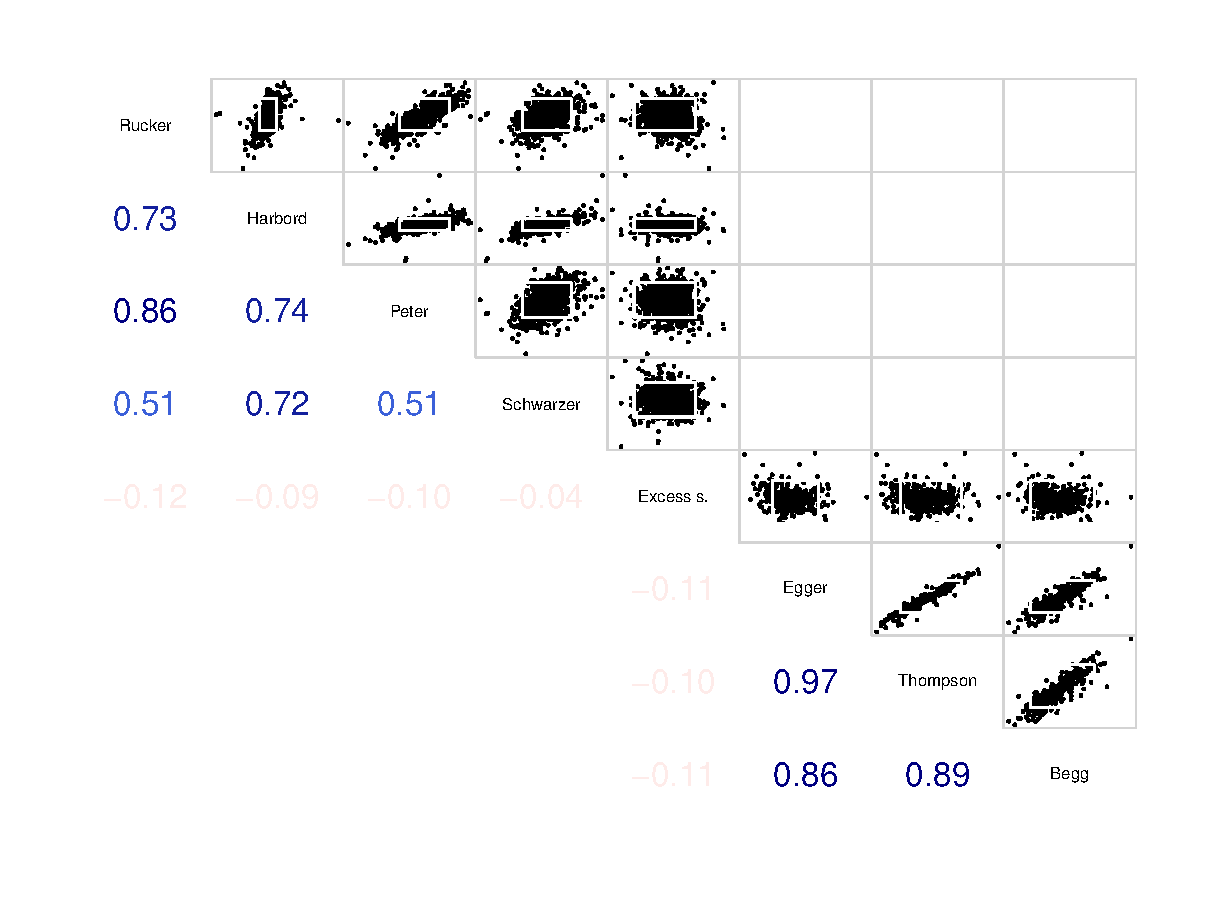
\includegraphics[width=\textwidth-3cm]{figure/ch03_figunnamed-chunk-11-1} 

}



\end{knitrout}
\caption{Median of the absolute Fisher's $z$ transformed correlation across sample size plotted against the total sample size.}
\label{z.samplesize}
\end{figure}

\begin{figure}
\begin{knitrout}
\definecolor{shadecolor}{rgb}{0.98, 0.98, 0.98}\color{fgcolor}

{\centering 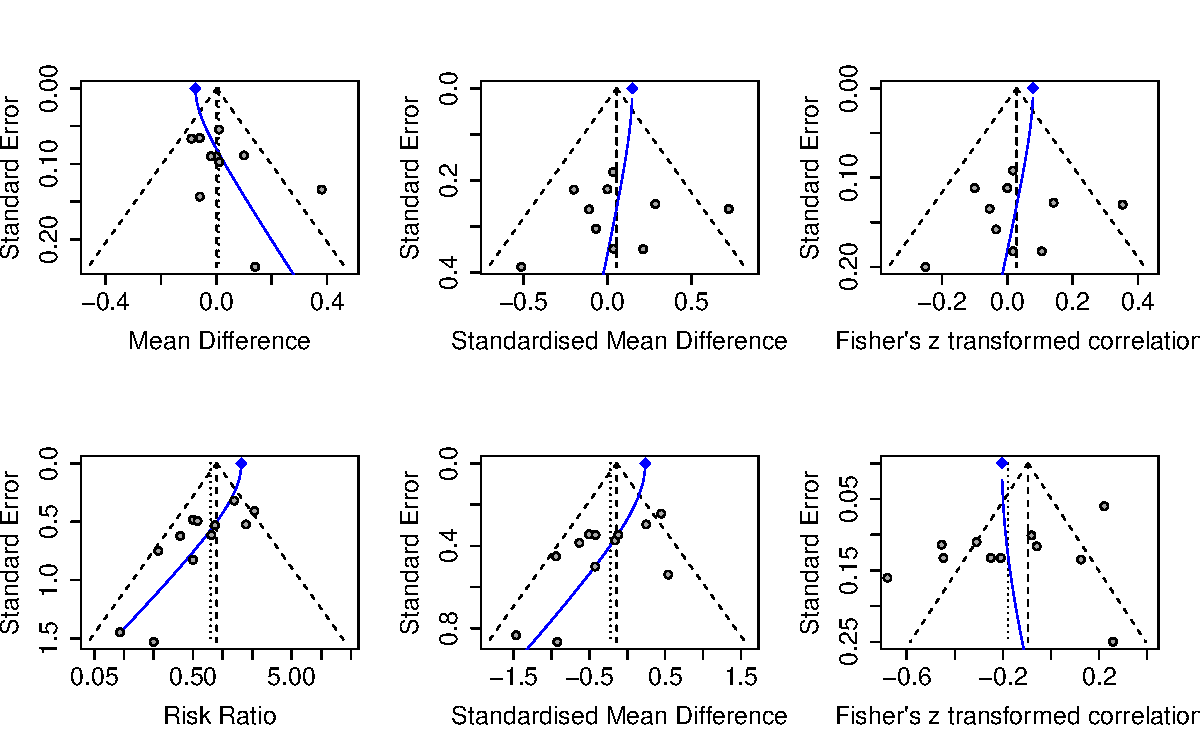
\includegraphics[width=\textwidth-3cm]{figure/ch03_figunnamed-chunk-12-1} 

}



\end{knitrout}
\caption{Median of the absolute value of the original effect size across sample size plotted against the total sample size.}
\label{effect.samplesize.separated}
\end{figure}



\section{Publication Bias Test Results} \label{sec:publication.bias.tests}




The meta-analyses fulfilling the criteria from Chapter \ref{ch:dataset}, section \ref{sec:Processing}, are analysed with one-sided small publication bias tests and excess significance tests. The direction in which bias is expected is the one on which more significant results of primary studies are (two-sided $p$-value < 0.05). The tests are applied on the original effect size measures, since the journal editors and the researchers also base their decisions on them. Different tests are applied depending on the outcome being binary or continuous or if the data is only partially available (\texttt{outcome.flag} = \texttt{IV}).\\
Multiple tests are applied in order to compare their results. A histogram of $p$-values for each test will summarize the overall evidence against the null-hypothesis of no publication bias, as displayed in Figure \ref{fig:test}.\\
The abbreviations in Figure \ref{fig:test}  are shortly explained with references to Chapter \ref{ch:methods}: \\
``Excess significance'' denotes the excess of significant $p$-values testing method from \citet{excess.significance}, see \ref{sec:excess.significance}. For continuous and \texttt{IV} outcomes, the names refer to: 

\begin{itemize}
\item Egger's test, weighted linear regression test described in Section \ref{sec:Egger}
\item Thompson and Sharp's test, weighted linear regression test adjusted for between-study heterogeneity, Section \ref{sec:Thompson}
\item Begg and Mazumdar's test, rank test described in Section \ref{sec:Begg}
\end{itemize}

For binary outcomes, the names refer to:
\begin{itemize}
\item Harbord's test, likelihood score based test (Section \ref{sec:Harbord})
\item Peter's test, weighted linear regression with inverse sample size as explanatory variable described in Section \ref{sec:Peter}
\item R\"ucker's test, test based on the arcsine transformation of proportions, in combination with Thompson and Sharp's regression test (Section \ref{sec:Rucker})
\item Schwarzer's test, rank based test using the expected event counts computed with the hypergeometric distribution (Section \ref{sec:Schwarzer})
\end{itemize}

\begin{figure}
\begin{knitrout}
\definecolor{shadecolor}{rgb}{0.98, 0.98, 0.98}\color{fgcolor}

{\centering 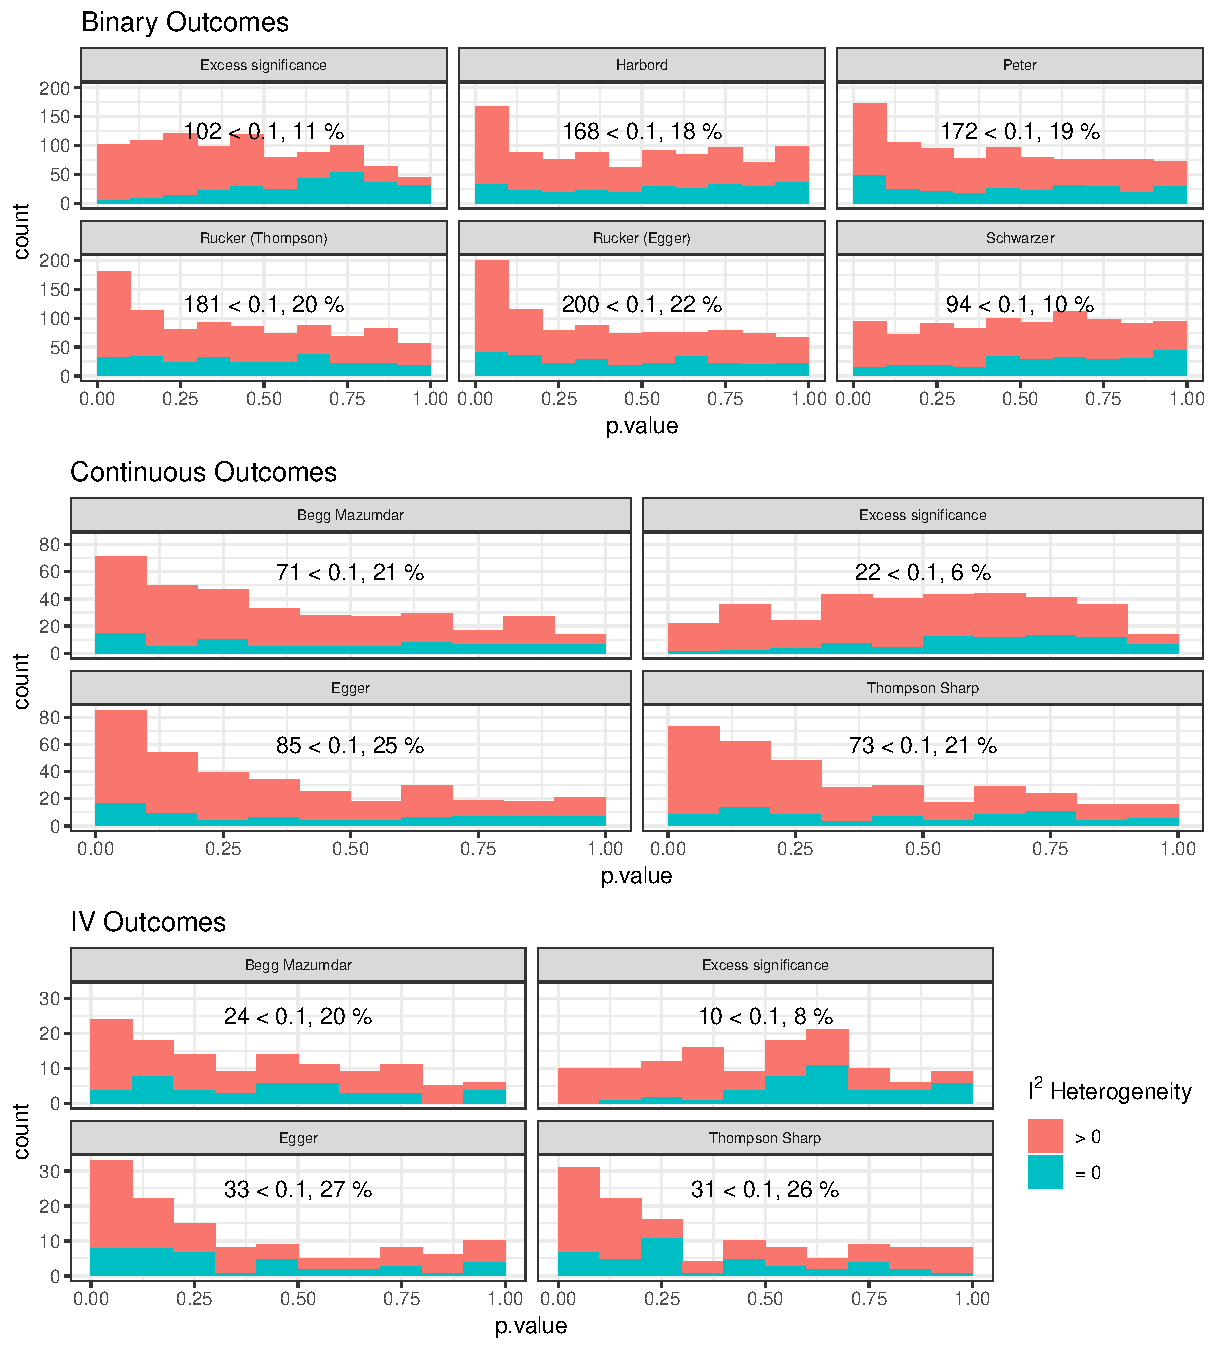
\includegraphics[width=\textwidth-3cm]{figure/ch03_figunnamed-chunk-14-1} 

}



\end{knitrout}
\caption{Histogram of one-sided $p$-values for small study effect in direction of larger effect sizes. The testing method is indicated in the header, bin width is equal to 0.1. The proportion of meta-analyses with significant publication bias based on the threshold of 0.1 is displayed inside the figures.}
\label{fig:test}
\end{figure}

%Agreement table -> Chunck 1
The histograms in Figure \ref{fig:test} show that the tests mostly find evidence for publication bias in the dataset. The $p$-values of excess significance and Schwarzer's test are rather uniformly distributed, but notably, excess significance test, Schwarzer's test and rank tests have been shown to lack statistical power. The tests that are more suitable (regression based tests in general) all have proportions of significant $p$-values ($p$ > 0.1) clearly above 10 \% which would be the expected false positive rate.\\
In Figure \ref{fig:test}, the meta-analyses with an estimated $I^2$ of zero are depicted, because some methods are known to only be suitable when no heterogeneity is present (excess significance test and also Egger's test). Other tests are specially constructed to adjust for between study heterogeneity (Thompson and Sharp's test and R\"ucker's test). These tests find a smaller proportion of significant results in Figure \ref{fig:test}. However, this is also due to application to meta-analyses with no between-study heterogeneity, where the methods lack statistical power. Similarly, the evidence decreases somewhat when R\"ucker's test is extended by Thompson and Sharp's method to account for heterogeneity. The moderate decrease indicates however that the previous restriction to meta-analyses with $I^2 < 0.5$ is sufficient to remove meta-analyses with large heterogeneity and that the test results are not heavily influenced by unaccounted between-study heterogeneity.\\
The $p$-values of tests can be summarized by computing their harmonic mean \citep{harmonic.p}. In the case of binary tests, the $p$-values of R\"ucker's, Peters, Harbord's, Schwarzer's and excess significance tests are used, in the case of continuous and \texttt{outcome.flag} = \texttt{IV} outcomes, Egger's, Thompson and Sharp's, Begg and Mazumdar's and excess significance tests are used. This lead's to an overall of 20.3\% significant results ($p_\textrm{harmonic}$ < 0.1, 19.7\% \texttt{outcome.flag} = \texttt{DICH}, 20.1\% \texttt{outcome.flag} = \texttt{CONT}, 25.6\% \texttt{outcome.flag} = \texttt{IV}).






\subsection{Publication Bias Test Consistency}
In a next step, the consistency between the tests is examined, \eg if the tests identify significant publication bias in the same meta-analyses. There is, so far, no agreement in the literature about which of the methods are to prefer, even non regression based tests have generally low power. The following analysis will reveal if there are \eg testing methods that are coming to identical results and are thus compatible/interchangeable. \\
A simple method to check the consistency of test results is to compare scatterplots and Spearman correlations between the test statistics. This is done in Figure \ref{fig:test.agreement}. Here, there is no separation between \texttt{IV} and continuous outcomes because the same publication bias tests have been used. The upper left rectangle is displaying binary outcome results and the lower right continuous and \texttt{IV} outcomes results. Also, the $I^2$ statistic is included. Since no normally distributed test statistic under the null hypothesis is used for excess significance tests, it is not shown here.

\begin{figure}
\begin{knitrout}
\definecolor{shadecolor}{rgb}{0.98, 0.98, 0.98}\color{fgcolor}

{\centering 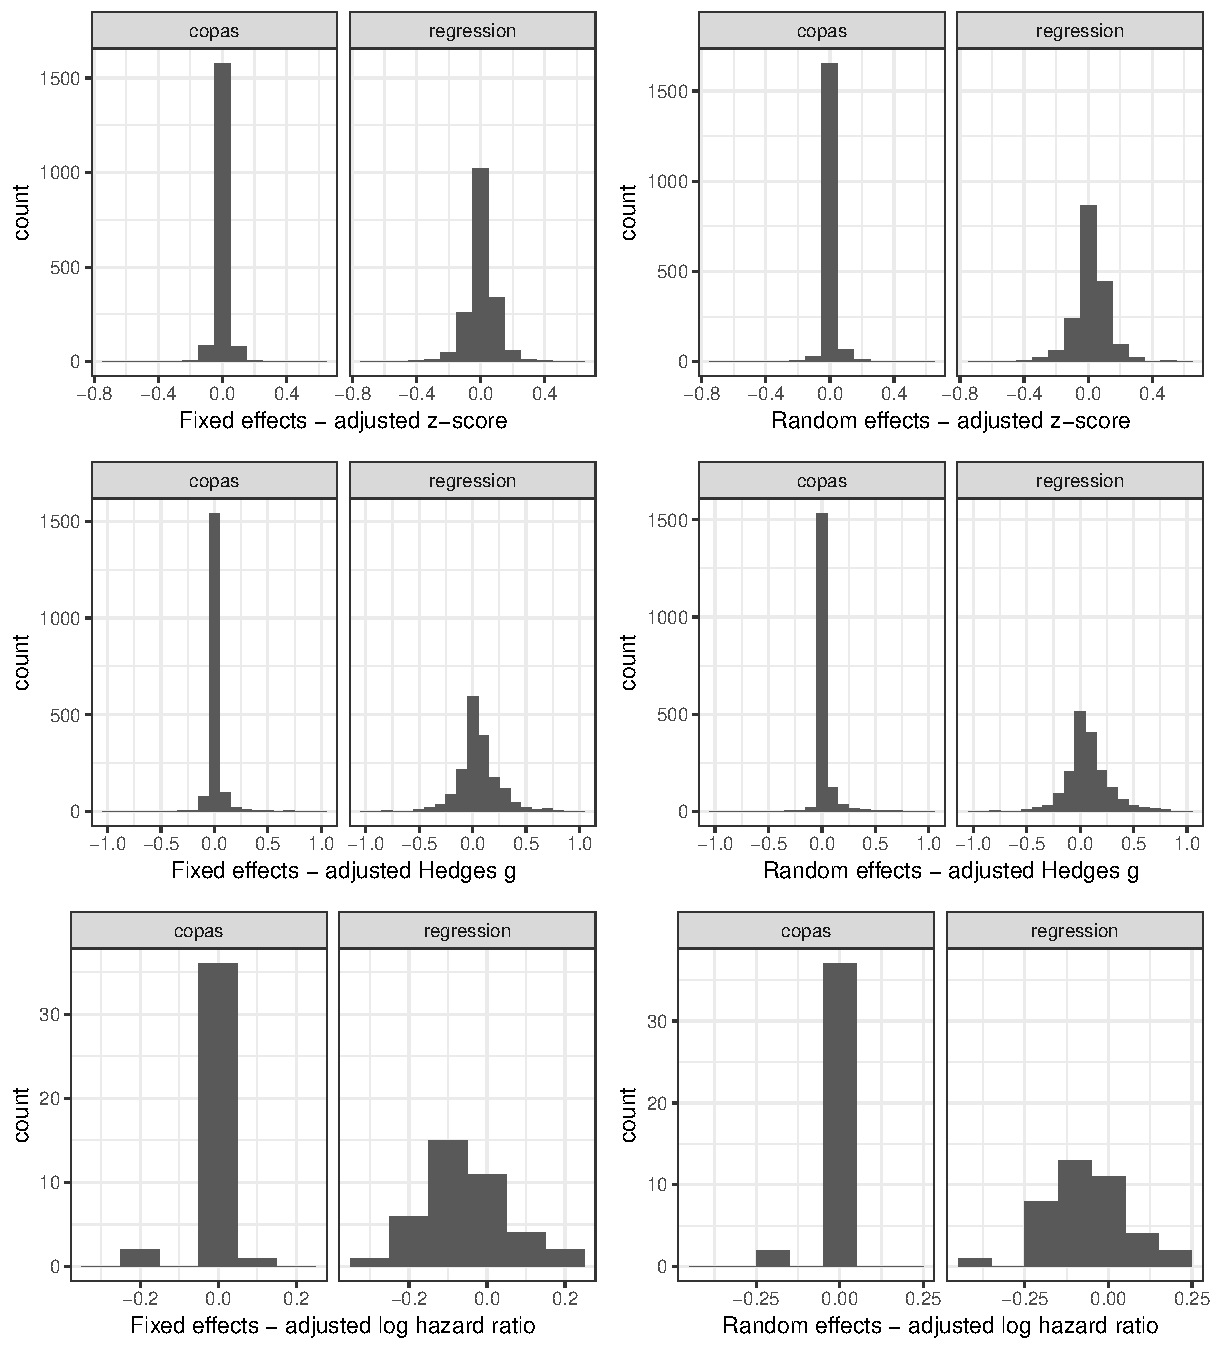
\includegraphics[width=\textwidth-3cm]{figure/ch03_figunnamed-chunk-15-1} 

}



\end{knitrout}
\caption{Pairs-plot for test statistics of small study effects. The lower panel gives the Spearman correlations for the different test statistics, and the upper panel displays a scatterplot. The colors indicate magnitude and direction of the correlation coefficients. The rectangle with white borders displays the area within which both tests have absolute value < 1.64 (dots inside are statistically not significant by 0.1 $p$-value threshold).}
\label{fig:test.agreement}
\end{figure}

The observed patterns on the scatterplots differ, and some methods do align better than others. Regression based tests as Egger and Thompsons test which are methodically almost identical are closely aligned, which is reflected in large correlation coefficients. Continuous and \texttt{IV} outcome type tests align more closely than binary outcome tests. While correlation coefficients between binary outcome tests vary between each other, Harbord's test statistic has similar correlation coefficients with the other small study effect test statistics.\\
Because scatterplots and correlation coefficients can be misleading, also a Tukey mean-difference or Bland-Altman of transformed $p$-values plot is shown for four scenarios in Figure \ref{fig:mean.diff.test}:
\begin{itemize}
\item For Egger's and Thompson's tests, which is supposedly the most similar test and should show the least deviations and systematic errors.
\item For Egger's and excess significance tests.
\item For Harbord's and R\"ucker's tests.
\item For Harbord's and excess significance tests.
\end{itemize}

This can be justified since all tests are supposed to measure the evidence for publication bias. For the plots, the $p$-values of the tests are transformed on the entire continuous scale by a logit transformation $f(x)  = \log(\frac{p}{1-p}$). The mean $p$-value (($f$($p$-value no. 1) + $f$($p$-value no. 2))/2) is then displayed against the difference between the $f$($p$-value). If no systematic errors and biases exist between the measurement methods, then 

\begin{itemize}
\item the mean of the differences should be around zero (no systematic error) 
\item the points should scatter independently on the $y$-axis and no general increase or decrease with the mean of the transformed $p$-values should be visible (and the linear regression fit is flat)
\end{itemize}

There are likely systematic errors and bias between the tests, although the extent seems to vary. Most error seems to be between small study effect tests and excess significance tests, because the slope of the linear regression fit is likely positive. This means that the excess significance test finds less evidence in cases when both $p$-values are small and more evidence when both $p$-values are large, on average.\\
However, the confidence intervals from Figure \ref{fig:mean.diff.test} are very large. This suggests that additionally to the bias correspondence between the tests is not very good in general. 

\begin{figure}
\begin{knitrout}
\definecolor{shadecolor}{rgb}{0.98, 0.98, 0.98}\color{fgcolor}

{\centering 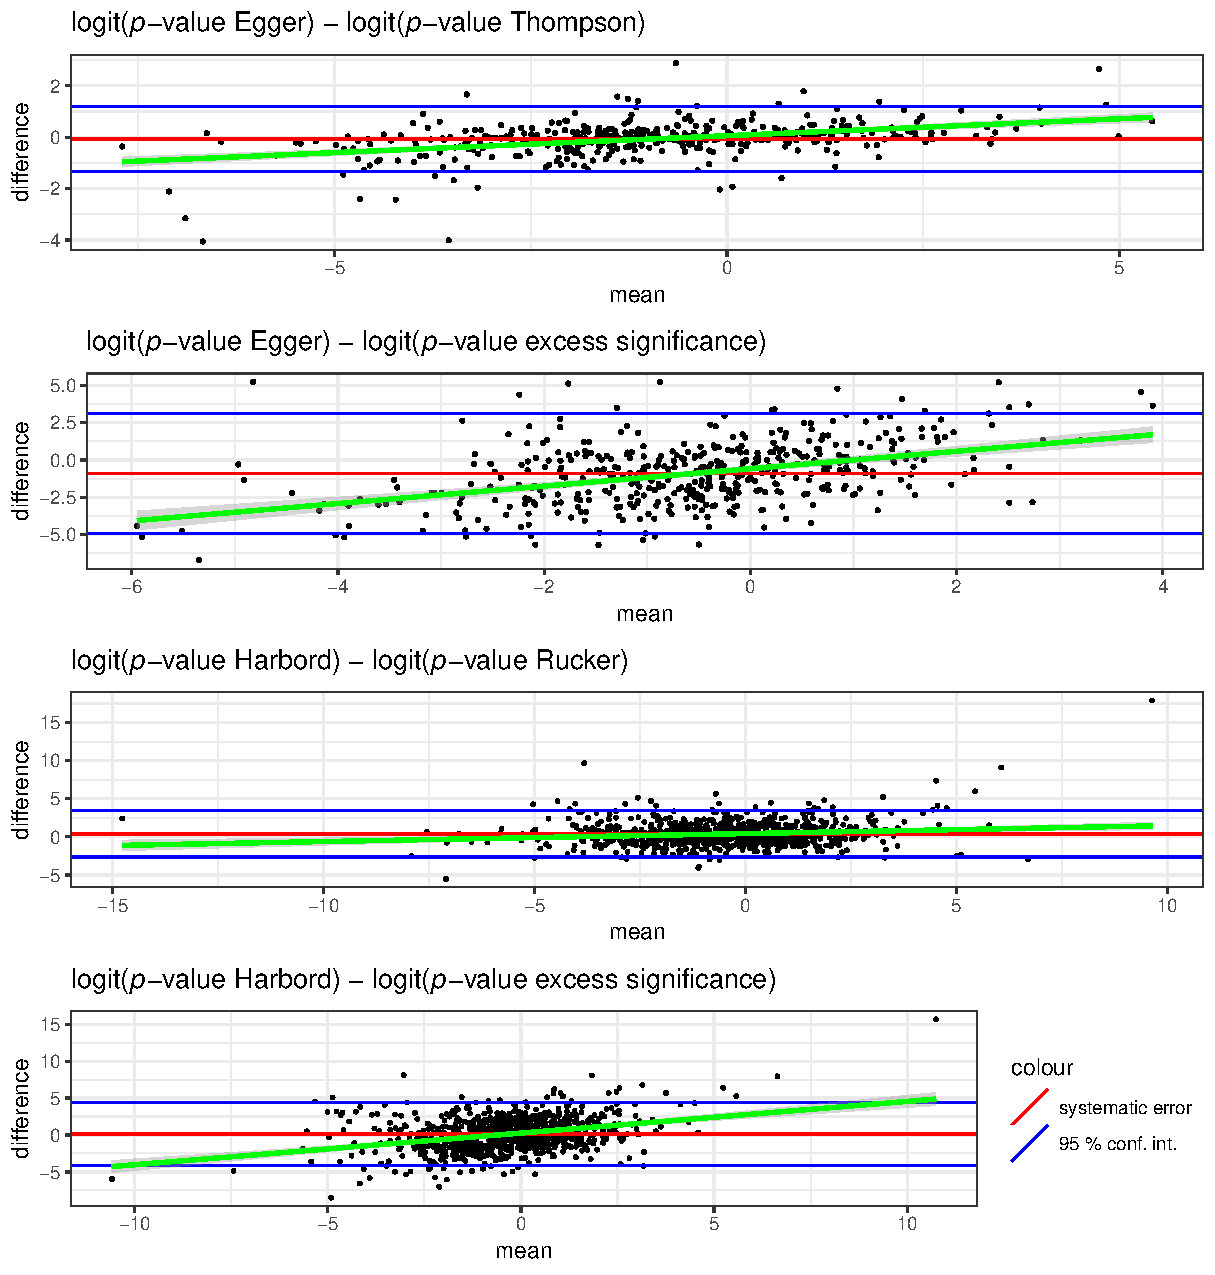
\includegraphics[width=\textwidth-3cm]{figure/ch03_figunnamed-chunk-16-1} 

}



\end{knitrout}
\caption{Mean - difference plots for logit transformed $p$-values. The mean of logit transformed $p$-values is displayed on the $x$-axis and the difference on the $y$-axis. Blue and red lines display the systematic error and the confidence intervals of the systematic error (limits of agreement).
In green, a linear regression fit is shown with 95\% CI bands.}
\label{fig:mean.diff.test}
\end{figure}

The previous results suggest that the results will also differ substantially after applying the common dichotomization of $p$-values. Some proportion of the meta-analyses will only be significant using a single test, while being non-significant otherwise. This can be seen in Table \ref{number.sig.tests}. It displays the percentage of meta-analyses with a certain number of significant test results. Very few meta-analyses are give a significant result, independently of the test applied. Around 67\% of the dataset is not significant, no matter which test is used. \\

% latex table generated in R 3.5.1 by xtable 1.8-3 package
% Thu Aug 15 22:03:09 2019
\begin{table}[ht]
\centering
\begingroup\footnotesize
\begin{tabular}{ccc}
  \hline
Count & Binary Outcomes & Continuous and IV \\ 
  \hline
0 & 66.1 \% & 65.3 \% \\ 
  1 & 12.3 \% & 11.9 \% \\ 
  2 & 7.7 \% & 6.9 \% \\ 
  3 & 6.8 \% & 14.2 \% \\ 
  4 & 5.7 \% & 1.7 \% \\ 
  5 & 1.3 \% & - \\ 
   \hline
\end{tabular}
\endgroup
\caption{Counts Number of significant test results per meta-analysis, separated
       for outcome types. Last entry for continuous and IV outcomes is empty since one test less was 
       applied} 
\label{number.sig.tests}
\end{table}


When leaving away the excess significance test, 29.5\% of binary outcome tests and 31.9\% of \texttt{IV} and continuous outcome tests had at least one significant result. 
%After applying the Bonferroni correction for multiple testing, this shrinks to mean.min.bin.b\% for binary and mean.min.else.b\% for continuous and \texttt{IV} outcomes. 
To compare significant findings for small study effect tests and excess significance tests, Harbord's or Egger's test results are compared with excess significance tests. 24.1\% of binary outcome analyses had at least one of the two test $p$-values being significant, and equivalently, 28.4\% for continuous and \texttt{IV} outcomes. The numbers change to 13.9\% for binary outcomes and 18.1\% for continuous and \texttt{IV} outcomes after applying the Bonferroni correction. 5.1\% have significant Harbord's test result and significant excess significance test result  (2.3\% with Bonferroni). Of the continuous outcomes, we have 3.9\% with Egger's test and 1.3\% with Bonferroni correction. \\
The precise proportions of agreement in significance/non-significance are provided in Table \ref{test.agreement}. A separate column provides the proportion of significant results of the test with fewer significant results that are also significant using the test with more significant results. 
Linear regression based tests agree more often with other linear regression based tests, and agreement between small study effect tests is in general well above 60 \% (at best, 95\% test agreement in significance for \texttt{IV} \texttt{outcome.flag}). The agreement on statistical significance between small study effect tests and excess significance tests ranges from 64\% to 4\% (for \texttt{IV} and rank tests). Note that these numbers are difficult to interpret because there are substantially less significant results of the excess significance tests, and thus, a agreement of 100\% still does not indicate perfect compatibility/replaceability of the tests.

% latex table generated in R 3.5.1 by xtable 1.8-3 package
% Thu Aug 15 22:03:09 2019
\begin{table}[ht]
\centering
\begingroup\scriptsize
\begin{tabular}{lcc}
  \hline
 & Agreement (overall) & Agreement (significance) \\ 
  \hline
Excess significance, Schwarzer & 0.85 & 0.27 \\ 
  Excess significance, Peter & 0.77 & 0.32 \\ 
  Excess significance, Rucker & 0.79 & 0.43 \\ 
  Excess significance, Harbord & 0.81 & 0.46 \\ 
  Peter, Schwarzer & 0.84 & 0.63 \\ 
  Schwarzer, Rucker & 0.85 & 0.72 \\ 
  Schwarzer, Harbord & 0.87 & 0.78 \\ 
  Rucker, Peter & 0.88 & 0.67 \\ 
  Harbord, Peter & 0.87 & 0.63 \\ 
  Excess significance, Egger & 0.77 & 0.64 \\ 
  Excess significance, Thompson & 0.80 & 0.59 \\ 
  Excess significance, Begg & 0.78 & 0.36 \\ 
  Thompson, Egger & 0.93 & 0.92 \\ 
  Thompson, Begg & 0.87 & 0.70 \\ 
  Egger, Begg & 0.84 & 0.70 \\ 
  Excess significance, Egger (IV) & 0.71 & 0.12 \\ 
  Excess significance, Thompson (IV) & 0.71 & 0.10 \\ 
  Excess significance, Begg (IV) & 0.74 & 0.04 \\ 
  Thompson, Egger (IV) & 0.95 & 0.94 \\ 
  Thompson, Begg (IV) & 0.86 & 0.79 \\ 
  Egger, Begg (IV) & 0.86 & 0.83 \\ 
   \hline
\end{tabular}
\endgroup
\caption{Overall proportion of agreement if publication bias is significant or non-significant, and if significant only. When comparing agreement if significant only, the proportion of the test with fewer significant results that is significant with another test as well is shown.} 
\label{test.agreement}
\end{table}





%%%%%%%%%%%%%%%%%%%%%%%%%%%%%%%%%%%%%%%%%%%%%%%%%%%%%%%%%%%%%%%%%%%%%%%%%%%%%%%%
%%%%%%%%%%%%%%%%%%%%%%%%%%%%%%%%%%%%%%%%%%%%%%%%%%%%%%%%%%%%%%%%%%%%%%%%%%%%%%%%
%%%%%%%%%%%%%%%%%%%%%%%%%%%%%%%%%%%%%%%%%%%%%%%%%%%%%%%%%%%%%%%%%%%%%%%%%%%%%%%%
%%%%%%%%%%%%%%%%%%%%%%%%%%%%%%%%%%%%%%%%%%%%%%%%%%%%%%%%%%%%%%%%%%%%%%%%%%%%%%%%
%%%%%%%%%%%%%%%%%%%%%%%%%%%%%%%%%%%%%%%%%%%%%%%%%%%%%%%%%%%%%%%%%%%%%%%%%%%%%%%%

\section{Small Study Effects Adjustment}


\subsection{Change in Effect Size after Adjustment} \label{sec:change.size}

There are methods that can take into account the presence of publication bias in meta-analyses when estimating the overall treatment effect. The methods work in a semi-automatic manner; they will not only adjust for publication bias if smaller studies show larger effects, but also in the opposite case. The latter results in the adjusted overall treatment effect being \textit{larger} than the unadjusted, overall treatment effect. \\
To compare the effects of adjustment between meta-analyses of different outcomes, the outcome measures are transformed to standardized mean differences and Fisher's $z$ transformed correlations (see section \ref{sec:transformation.effectsizes} for details). When comparing to unadjusted effects, fixed or random effects meta-analysis estimates are used as references\\
Figure \ref{fig:adjustment.reg} displays the difference between the estimated meta-analysis treatment effect and the regression adjusted treatment effect \ref{sec:regression.adjustment}, $\hat{\theta}_M - \hat{\theta}_\textrm{Adj.}$. The absolute value $|\hat{\theta}_M|$ is taken and $\hat{\theta}_\textrm{Adj.}$ is negative if it's sign is different from the sign of the original $\hat{\theta}_M$. Thus, a positive difference indicates a reduction of the original effect size, and the magnitude of the difference indicates the extent of the adjustment. \\
Additionally, the test statistics of heterogeneity adjusted publication bias tests (R\"ucker's and Thompson's test) are displayed with green color. Test statitics smaller $t < 1$ (light green colored) are equivalent to no evidence for publication bias, test statistics $t$ between one and two to weak evidence, and above two they indicate evidence for publication bias (dark green). An adjusted effect with evidence for publication bias can be regarded as a more realistic estimate of the treatment effect. Some very large and very small differences have been omitted in the Fisher's $z$ transformed correlation and std. mean difference histograms; they are shown in Table \ref{missing.differences}. \\
Most often, adjustment leads to a reduction of overall treatment effect estimates, which can be seen by the size of the bins on the positive side of the histograms. Adjustment is stronger when random effects meta-analysis is used as reference, because it gives larger weights to small studies.\\
Contrary to naive expectation, we see cases with large negative adjustment, but no evidence for small study effects. This is because the linear regression parameter estimates are large, but estimated with high uncertainty, such that there will be few evidence for small study effects (publication bias), but nonetheless, the adjustment will be large. It is recommended to use the methods only in cases where there is clear evidence for publication bias. The color legend in Figure \ref{fig:adjustment.reg} thus gives a sense of the confidence that is put into the adjusted effects. \\

\begin{figure}
\begin{knitrout}
\definecolor{shadecolor}{rgb}{0.98, 0.98, 0.98}\color{fgcolor}

{\centering 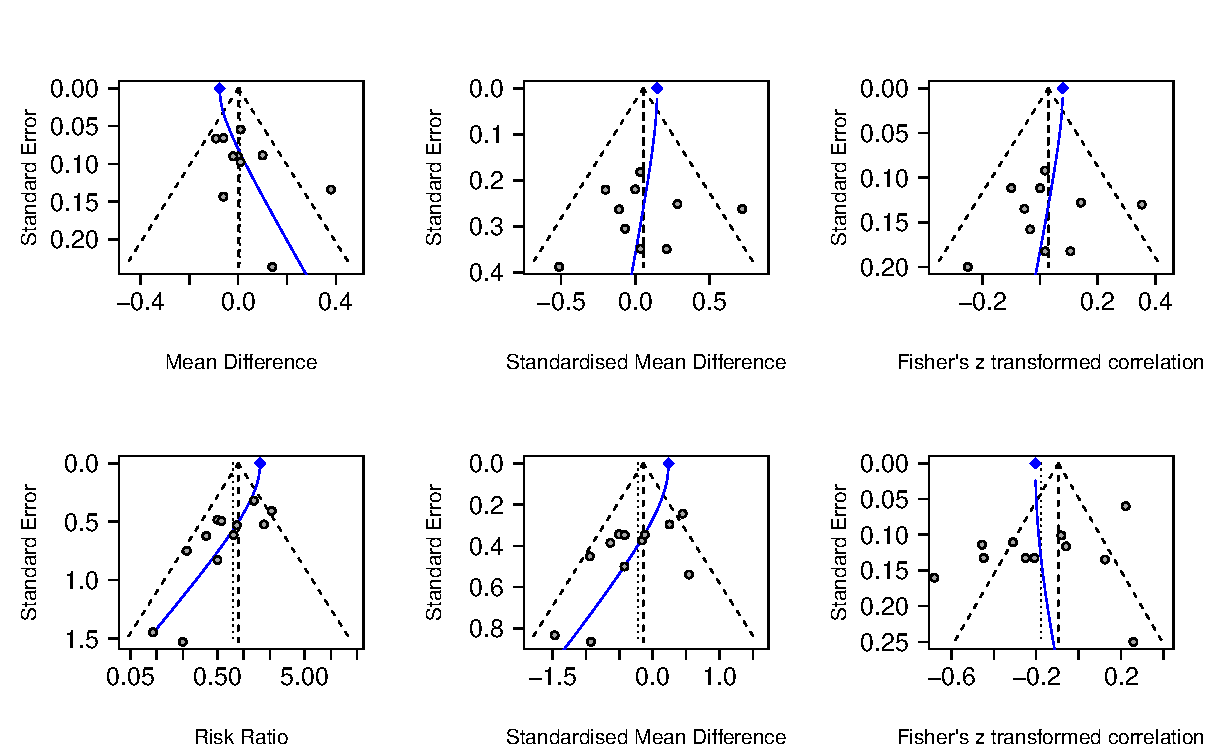
\includegraphics[width=\textwidth-3cm]{figure/ch03_figunnamed-chunk-20-1} 

}



\end{knitrout}
\caption{Histogram of the treatment effect differences between meta-analysis and regression adjusted meta-analysis. Negative differences indicate greater adjusted effect sizes than meta-analysis effect sizes. The bins are centered at zero and binwidth is equal to 0.1. Deeper green color indicates more evidence for small study effects.}
\label{fig:adjustment.reg}
\end{figure}

Additionally, some meta-analyses with positively adjusted, larger overall treatment effects after adjustment (left side of the histogram) have also evidence for publication bias (defined as the tendency of small studies to show \textit{larger} results because only significant results are published). However, this is not wrong, because the effects and their variances have been transformed, and it is possible that the shape of the funnel plot changes upon transformation; Figure \ref{fig:funnel.plot.change} shows this for illustrative purposes. From the left to the right, the funnel plot is shown for mean differences (the original measure), standardized mean differences and Fisher's $z$ scores; there is no change upon adjustment using mean differences (blue line), reduction of the effect with std. mean differences and increase with Fisher's $z$ transformed correlation. Note that while the rank of the effect sizes is usually preserved after transformation, the relative size and especially the variance may vary. One effect of the Fisher's $z$-transformation is that the effect sizes are bounded on $[-1,1]$, and thus, very large effect sizes will influence the fit of the linear regression less than for example in std. mean differences, which are not bounded. In contrast, the variance of the correlation is directly tied to the sample size, which makes it a suitable proxy for study size (variance of the mean difference is in contrast strongly influenced by the standard deviations).

\begin{figure}
\begin{knitrout}
\definecolor{shadecolor}{rgb}{0.98, 0.98, 0.98}\color{fgcolor}

{\centering 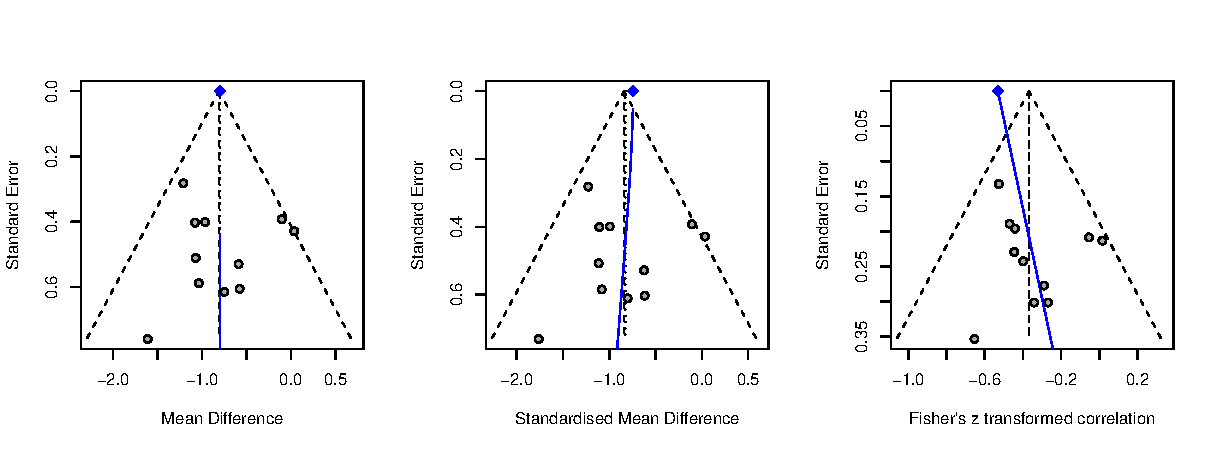
\includegraphics[width=\textwidth-3cm]{figure/ch03_figunnamed-chunk-21-1} 

}



\end{knitrout}
\caption{Funnel plots for a meta-analysis based on three different effect size measures: Mean differences, std. mean differences and Fisher's z transformed correlations and corresponding standard errors. Vertical dashed lines indicate meta-analysis estimates, the rhombus with the curved blue line the adjusted treatment effect.}
\label{fig:funnel.plot.change}
\end{figure}


Figure \ref{fig:adjustment.copas} shows the differences between Meta-analysis and adjusted effect sizes adjusted by Copas selection model; the model substitutes its estimates with random effect estimates when it finds no evidence for small study effects. Therefore, the effect of adjustment by Copas can better be seen when comparing adjusted with random effects meta analysis estimates. Again, we clearly see that more effect sizes are adjusted downwards. Additionally, there is more coincidence between publication bias test statistics and adjustment, \ie positive differences are accompanied by large positive test statistics, which is as expected. \\
Table \ref{adjustment.difference} shows quantiles and means for the various differences and the overall proportion of downward adjusted effect sizes. When std. mean difference is used as an effect measure, there are (substantially) more reduced effect sizes. The means in Table \ref{adjustment.difference} suggest that the average reduction is small. To recall some other findings out of Table \ref{adjustment.difference}: 5\% or 69 meta-analyses have their Fisher's $z$ transformed correlation reduced by more than 0.13 by regression adjustment (and 5\% or 69 increased by -0.11 or more, fixed effects reference). Also, std. mean difference is reduced by 0.39 compared to fixed effects estimates in 5\% or 69 meta-analyses (or increased by 0.24). 

\begin{figure}
\begin{knitrout}
\definecolor{shadecolor}{rgb}{0.98, 0.98, 0.98}\color{fgcolor}

{\centering 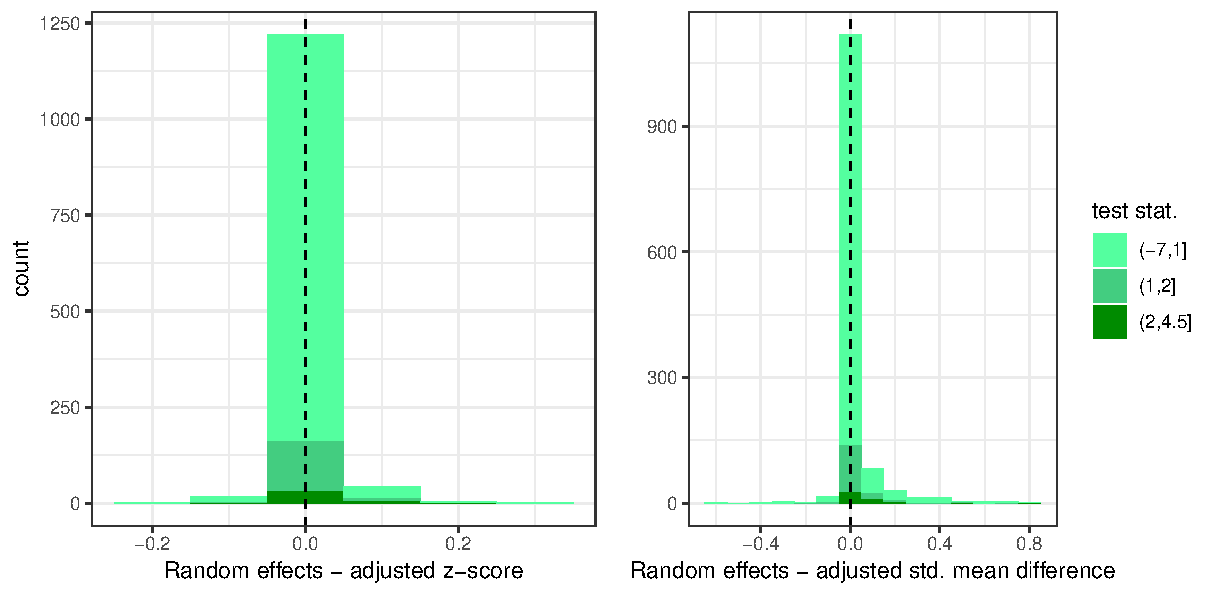
\includegraphics[width=\textwidth-3cm]{figure/ch03_figunnamed-chunk-22-1} 

}



\end{knitrout}
\caption{Histogram of the treatment effect differences between meta-analysis and Copas adjusted meta-analysis. Negative differences indicate greater adjusted effect sizes than meta-analysis effect sizes. The bins are centered at zero and binwidth is equal to 0.1. Deeper green color indicates more evidence for small study effects.}
\label{fig:adjustment.copas}
\end{figure}

% latex table generated in R 3.5.1 by xtable 1.8-3 package
% Thu Aug 15 22:03:23 2019
\begin{table}[ht]
\centering
\begingroup\scriptsize
\begin{tabular}{lcccccccccr}
  \hline
 & 5\% & 25\% & 50\% & 75\% & 95\% & mean & = 0 (\%) & $>$= 0 (\%) & $>$ 0 (\%) & No adj. est. (\%) \\ 
  \hline
z: Fixed - Copas & -0.04 & -0.01 & 0.00 & 0.01 & 0.04 & 0.00 & 8.14 & 50.14 & 42.00 & 65.49 \\ 
  z: Random - Copas & -0.00 & 0.00 & 0.00 & 0.00 & 0.04 & 0.00 & 67.15 & 85.23 & 18.08 & 65.49 \\ 
  z: Fixed - Regression & -0.11 & -0.03 & 0.01 & 0.05 & 0.13 & 0.01 & 0.00 & 52.02 & 52.02 & 0.00 \\ 
  z: Random - Regression & -0.13 & -0.02 & 0.02 & 0.06 & 0.16 & 0.02 & 0.00 & 56.56 & 56.56 & 0.00 \\ 
  d: Fixed - Copas & -0.05 & -0.01 & 0.00 & 0.01 & 0.11 & 0.01 & 19.38 & 56.41 & 37.03 & 56.92 \\ 
  d: Random - Copas & -0.00 & 0.00 & 0.00 & 0.00 & 0.16 & 0.02 & 60.09 & 85.01 & 24.93 & 56.92 \\ 
  d: Fixed - Regression & -0.21 & -0.03 & 0.04 & 0.14 & 0.40 & 0.06 & 0.00 & 60.16 & 60.16 & 0.00 \\ 
  d: Random - Regression & -0.20 & -0.02 & 0.05 & 0.17 & 0.44 & 0.08 & 0.00 & 62.68 & 62.68 & 0.00 \\ 
  IV: Fixed - Copas & -0.06 & -0.01 & 0.00 & 0.01 & 0.07 & 0.00 & 23.97 & 42.15 & 66.12 & 59.50 \\ 
  IV: Random - Copas & -0.00 & 0.00 & 0.00 & 0.01 & 0.08 & 0.01 & 61.98 & 28.93 & 90.91 & 59.50 \\ 
  IV: Fixed - Regression & -0.24 & -0.02 & 0.03 & 0.11 & 0.36 & 0.03 & 0.00 & 66.12 & 66.12 & 0.00 \\ 
  IV: Random - Regression & -0.25 & -0.02 & 0.04 & 0.13 & 0.49 & 0.05 & 0.00 & 68.59 & 68.59 & 0.00 \\ 
   \hline
\end{tabular}
\endgroup
\caption{Quantiles and means of the differences between meta-analysis combined treatment effects and small study adjusted treatment effects. The column with the names ``> 0'' give the percentages of estimates larger than zero or larger or equal zero. The column ``No adj. est.'' gives the percentage of missing estimates due to non-significant publication bias test (for Copas) and computational errors. The row names indicate which outcome measure, meta-analysis method and adjustment method is used. Abbreviations are used for Fisher's z transformed correlation (z) and std. mean difference (d). Separate rows give the results for IV outcomes, where the original effect sizes (log rate ratios, hazard ratios, etc.) are used.} 
\label{adjustment.difference}
\end{table}



% latex table generated in R 3.5.1 by xtable 1.8-3 package
% Thu Aug 15 22:03:23 2019
\begin{table}[ht]
\centering
\begingroup\tiny
\begin{tabular}{cccrrrrrrrr}
  \hline
id & comparison.nr & subgroup.nr & z fixed & z random & z Copas & z reg. & smd fixed & smd random & smd Copas & smd reg. \\ 
  \hline
CD000370 & 8 & 2 & 0.66 & 0.66 & 0.66 & 0.82 & 1.59 & 1.59 & 1.40 & 0.28 \\ 
  CD001183 & 7 & 0 & -0.48 & -0.48 & -0.48 & -0.21 & -1.10 & -1.12 & -0.50 & -0.11 \\ 
  CD002307 & 2 & 1 & -0.10 & -0.08 & -0.10 & 0.03 & -0.47 & -0.42 & -0.41 & -3.00 \\ 
  CD008625 & 2 & 2 & -0.60 & -0.60 & -0.60 & -0.39 & -1.72 & -2.02 & -1.01 & -0.69 \\ 
  CD010060 & 1 & 0 & 0.31 & 0.32 & 0.31 & 0.23 & 0.50 & 0.52 & 0.20 & -0.49 \\ 
   \hline
\end{tabular}
\endgroup
\caption{Missing meta-analysis combined treatment effect and adjusted treatment effects. Abbreviations are used for Fisher's z transformed correlation (= z) and std. mean difference (= d).} 
\label{missing.differences}
\end{table}



\subsection{Comparison of adjustment methods}
Regression adjusted estimates are compared to the estimates of Copas selection model if these are not equal to random effects meta-analysis in Figure \ref{fig:adjustment.mean.diff}. A Tukey mean difference plot can reveal systematic differences and biases between the two measurement methods. Note that only 26 out of 121 \texttt{IV} outcome data is included when using Fisher's $z$ transformed correlation and std. mean differences, since not all effects could be transformed.

\begin{figure}
\begin{knitrout}
\definecolor{shadecolor}{rgb}{0.98, 0.98, 0.98}\color{fgcolor}

{\centering 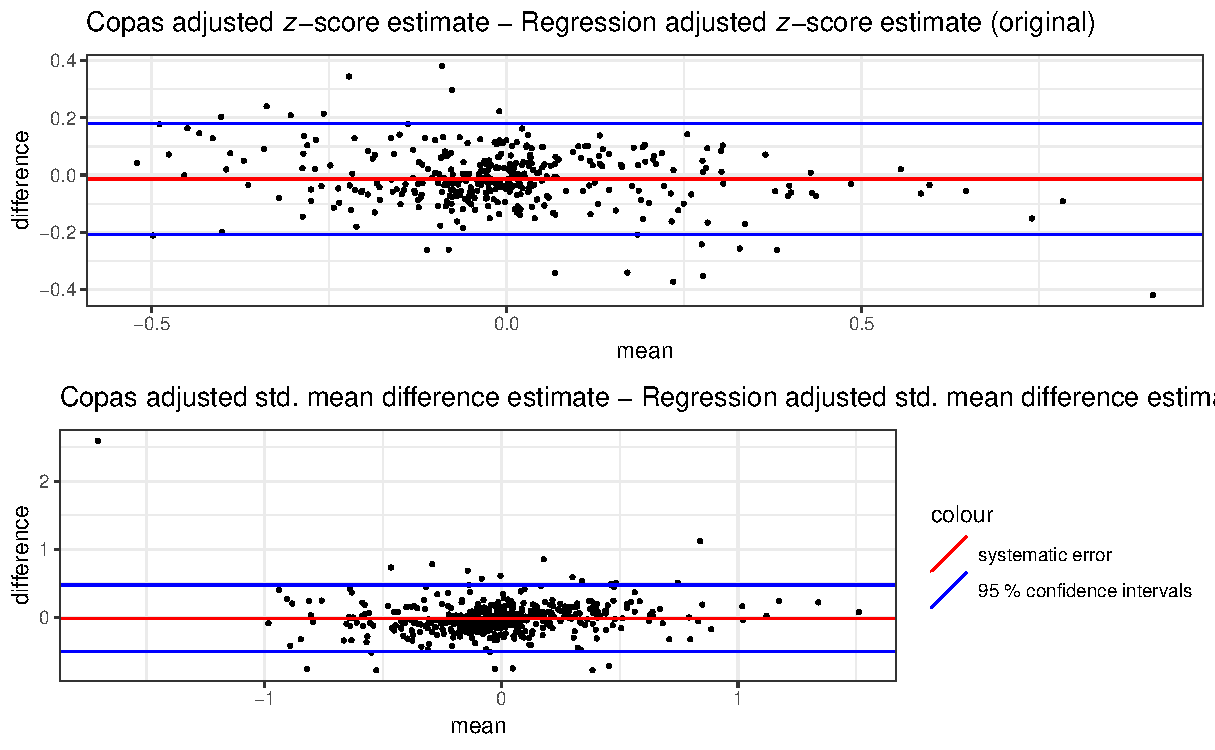
\includegraphics[width=\textwidth-3cm]{figure/ch03_figunnamed-chunk-25-1} 

}



\end{knitrout}
\caption{Mean - difference plots for publication bias adjustment methods. The mean of the adjusted treatment effects is displayed on the $x$-axis and the difference on the $y$-axis. Blue and red lines display the systematic error and the confidence intervals of the systematic error (limits of agreement). Two values have been omitted in the middle plot for std. mean difference and one for Fisher's $z$ transformed correlation (see Table \ref{missing.differences}).}
\label{fig:adjustment.mean.diff}
\end{figure}

No formal tests are provided, but the at least there seems to be no clear bias or systematic error. The limits of agreement in Figure \ref{fig:adjustment.mean.diff} are large. We conclude thus that the impact of regression adjustment on the effect sizes is in general not substantially larger than the impact of Copas selection model in the subset of data where the estimate of the Copas selection model is not equal to a random effects estimate. There is however a small difference, indicating that regression estimates have a little bit a larger absolute value. There might be some bias between adjusted Fisher's $z$ transformed correlations, where regression estimates seem to be somewhat smaller when the mean is a little above zero, and somewhat larger when the mean is a little below zero. \\


\subsection{Change in Evidence for Treatment Effects} \label{sec:change.evidence}
Adjustment for small study effects in meta-analysis will provide new effect sizes and standard errors. The evidence against the null hypothesis of no treatment effect can be computed newly. The test statistics $\frac{\theta}{\se(\theta)}$ of random effects and fixed effects meta-analysis and the corresponding adjusted test statistics are shown in Figure \ref{fig:evidence.adjustment}. The original scale of the effects sizes is used, since it is the measure on which policy-makers assess the treatment efficacy.

\begin{figure}
\begin{knitrout}
\definecolor{shadecolor}{rgb}{0.98, 0.98, 0.98}\color{fgcolor}

{\centering 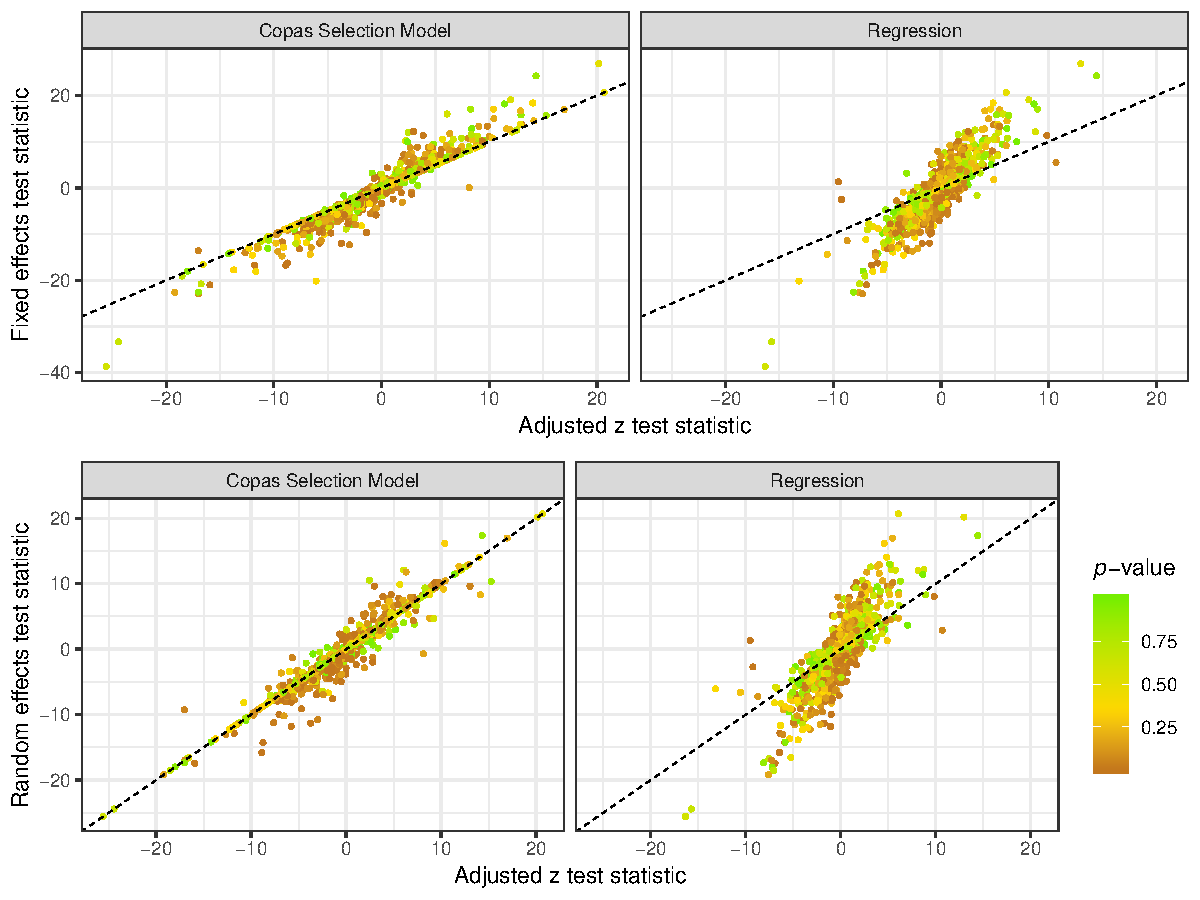
\includegraphics[width=\textwidth-3cm]{figure/ch03_figunnamed-chunk-26-1} 

}



\end{knitrout}
\caption{Test statistics of meta-analyses before and after adjustment. The color indicates the evidence for publication bias (\textit{p}-value of R\"ucker's or Egger's test), and the dotted line depicts the diagonal through the origin. Together with the horizontal dotted lines, the area which it borders indicates the consequences of adjustment for the evidence for a treatment effect. ``decrease'' means that the test statistic is smaller upon adjustment, ''increase'' that it is larger.}
\label{fig:evidence.adjustment}
\end{figure}

% Points lying on the diagonal through the origin indicate that there is no change in evidence after adjustment. In a hypothetical study with all treatment effects being artifacts of publication bias and perfect adjustment methods, all points should be distibuted on a vertical line at $x = 0$. A mitigation of evidence against the null hypothesis after adjustment thus is indicated by the adjusted test statistics being closer to zero. \\

The areas that are bordered by the diagonal and horizontal lines indicate which are the consequences of adjustment for a dot within. ``decrease'' indicates fewer evidence for treatment effect is given after adjustment, ''increase'' that adjustment led to larger evidence for treatment effects. \\
It can be seen that the alignment on the diagonal changes depending on the adjustment method. The effect of adjustment by Copas can be seen when comparing it to random effects meta-analysis. There, less of an effect of adjustment on the evidence can be seen. The adjustment is more likely to be more reliable than the unadjusted estimate when publication bias is strong (see \ref{ch:methods}). The dots with darker color are thus more likely to provide less biased estimates.\\
The decrease in evidence is larger when using adjustment with regression, which can be expected as the uncertainty of the additional parameter from the linear regression fit to estimate publication bias is included in the uncertainty of the estimate. In contrast, as the Copas selection model algorithm does a sensitivity analysis, the uncertainty of additional model parameters does not affect the estimate as they are not estimated but treated as fixed (see section \ref{sec:procedure} and section \ref{sec:copas}).\\
Large adjustment in effect sizes and test statistics is not necessarily accompanied by evidence for publication bias (color of the dots) in regression adjustment, as already discussed. But the dark dots can be found more often far away from the diagonal. Some cases which have more evidence for treatment efficacy after adjustment have evidence for publication bias, although the publication bias tests applied are one-sided and only test for bias towards large effects. This is because the algorithm to detect the side on which publication bias was expected (section \ref{sec:procedure}) has failed, \eg because few significant effects are given (used to define side of bias) and the weighted mean effect is close to zero, in which case it is difficult to decide upon the side of publication bias. There are some adjustments with large increase in evidence and clear dark orange color, as in the plots on the right hand side in Figure \ref{fig:evidence.adjustment}. Two of them are investigated in detail. 
\begin{itemize}
\item z test statistic of regression adjustment 10.5 vs fixed effects z test statistic 5.7: When the funnel plot of these meta-analyses are investigated, it becomes clear that there is no reason to assume publication bias since the smaller studies are near to risk ratios equal to one, and larger studies show larger ratios. Publication bias tests disagree in their findings (R\"ucker's and Harbord's tests: 0.058 and 0.05, and Peters and Schwarzer's test: 0.467 and 0.79).
\item z test statistic of regression adjustment 9.24 vs fixed effects z test statistic 2.51: Asymmetry of the funnel plot could be confirmed when analyzing it with mean differences. The change to a larger treatment effect is rather due to large between study heterogeneity and the specific routine of the regression adjustment. Because it takes into account between-study heterogeneity (bias parameter times $\tau^2$), while fixed effects meta-analysis does not, it returns a larger treatment effect. The adjusted effect (MD = - 10.3) lies between the fixed effect estimate (-2.56) and the random effects estimate (-18.7).
\end{itemize}
In the case of Copas selection model and when both test statistics are large (> 10), the explanation lies in a specialty of the model; the adjusted treatment effect estimates are not larger than the unadjusted, but their standard errors are different and sometimes smaller, because they are obtained from the Fisher information matrix of the log-likelihood (see subsection \ref{sec:copas}). \\
The Copas selection model also allows to compute the number of missing (\ie unpublished) studies in a given meta-analysis, given that the model's assumptions are correct. It finds that 2,618 are missing, which corresponds to 11.4\% from all 22,916 analysed studies. Figure \ref{fig:copas.missing} shows a histogram of the overall fraction of missing studies. Note that random effects meta-analysis substitutes have been excluded (828 out of 1,388 to limit the size of the bin at no. missing studies = 0.

\begin{figure}
\begin{knitrout}
\definecolor{shadecolor}{rgb}{0.98, 0.98, 0.98}\color{fgcolor}

{\centering 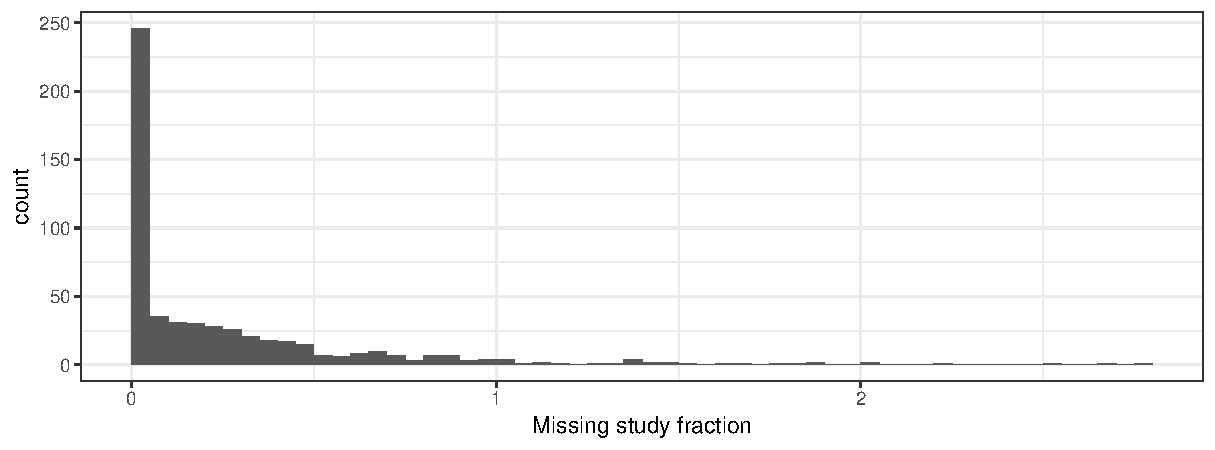
\includegraphics[width=\textwidth-3cm]{figure/ch03_figunnamed-chunk-27-1} 

}



\end{knitrout}
\caption{Histogram of the fraction of missing studies from the total number of studies in a meta-analyses (only data shown where Copas estimate was obtained, thus \\$n =$ 560)}
\label{fig:copas.missing}
\end{figure}

We can see that in some occasions, the method finds more than half of all studies in a meta-analysis are missing. In most occasions, the estimate of missing studies is zero, as can be seen in Table \ref{copas.missing}, where both the absolute number of missing studies and the fraction of missing studies in a meta-analysis are given. The discrepancy between mean and median may indicate that the estimate of 11.4\% missing studies depends somewhat on these extreme cases. As can be written of from Table \ref{copas.missing}, 5\%, \ie 28 meta-analyses have 17.6 or more studies missing: in fact, these 5\% most extreme make up for 1,060, more than 30\% of all missing studies.

% latex table generated in R 3.5.1 by xtable 1.8-3 package
% Thu Aug 15 22:03:25 2019
\begin{table}[ht]
\centering
\begingroup\footnotesize
\begin{tabular}{lrrrrrrr}
  \hline
 & = 0 & 5\% & 25\% & 50\% & 75\% & 95\% & mean \\ 
  \hline
Missing fraction & 226 & 0 & 0 & 0.1 & 0.4 & 1.0 & 0.3 \\ 
  Missing study number & 226 & 0 & 0 & 1.5 & 5.9 & 20.1 & 4.7 \\ 
   \hline
\end{tabular}
\endgroup
\caption{Fraction of missing studies and estimates of missing studies with their zero counts (``= 0''), quantiles and means.} 
\label{copas.missing}
\end{table}




\section{Mixed Effect Models and Publication Bias over Time}
To test if publication bias in meta-analyses has changed over time and newer meta-analyses have less bias, a generalized linear model has been set up to analyze all meta-analyses jointly and estimate a single parameter denoting publication bias. The procedure is to first start with the simplest model and consecutively add more explanatory variables and check by means of the AIC, BIC and F-test if the fit of the model has improved.\\
The dependent variable is the standardized mean differences(therefore, from \texttt{outcome.flag} = \texttt{IV}, only the std. mean differences are used). As before in section \ref{sec:change.size}, the std. mean difference is mirrored to one side by multiplying with the sign of the expected side of bias, \ie -1 or 1. \\
In a first step, the explanatory variable is the standard error, and the weights are the inverse of the variance of the std. mean difference. Additionally, random effects for the meta-analysis and for the review are added, the former being nested in the latter. Figure \ref{fig:smds} shows the complete dataset with the fit of the previously described model (dotted red line). The details and evidence for the small study effects in the generalized linear model are given in Table \ref{anova.small.study}, the coefficients in Table \ref{coefficients.small.study}

\begin{figure}
\begin{knitrout}
\definecolor{shadecolor}{rgb}{0.98, 0.98, 0.98}\color{fgcolor}

{\centering 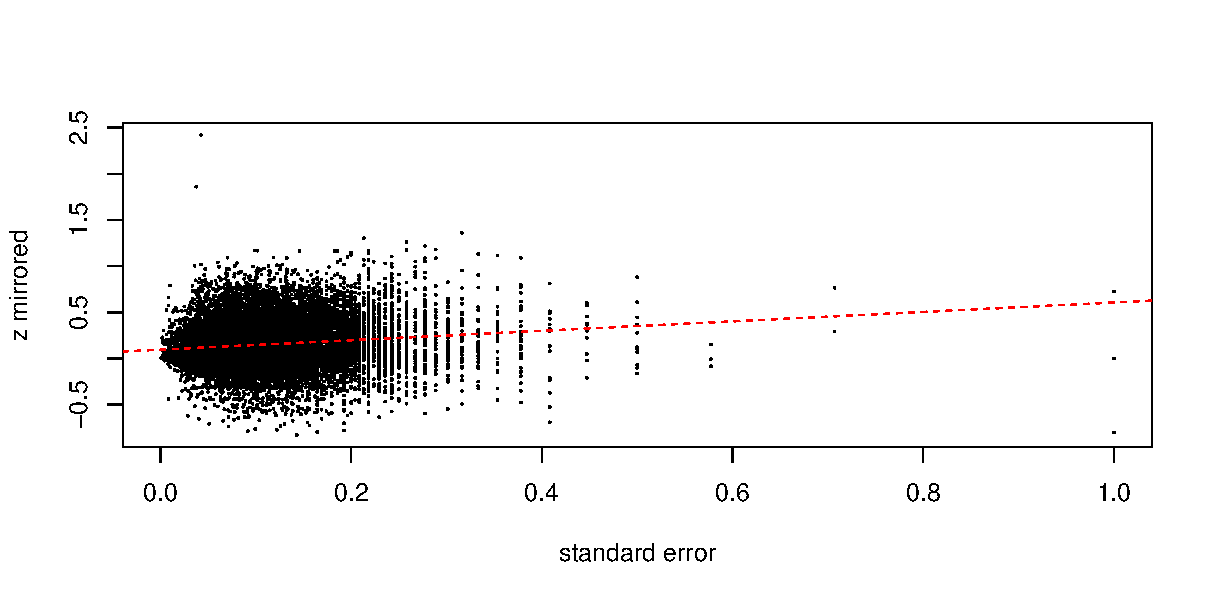
\includegraphics[width=\textwidth-3cm]{figure/ch03_figunnamed-chunk-29-1} 

}



\end{knitrout}
\caption{Std. mean differences of all meta-analyses plotted against their standard error, with the fit of a generalized linear model (dotted red line).}
\label{fig:smds}
\end{figure}

% latex table generated in R 3.5.1 by xtable 1.8-3 package
% Thu Aug 15 22:03:33 2019
\begin{table}[ht]
\centering
\begingroup\scriptsize
\begin{tabular}{rrrrrrlrl}
  \hline
 & Model & df & AIC & BIC & logLik & Test & L.Ratio & p-value \\ 
  \hline
null.fit &  1 & 4.0 & 18768.2 & 18800.1 & -9380.1 &  &  &  \\ 
  publication.bias.fit &  2 & 5.0 & 18230.5 & 18270.4 & -9110.3 & 1 vs 2 & 539.7 & $<$0.00001 \\ 
   \hline
\end{tabular}
\endgroup
\caption{Anova table for a generalized linear model for small study effects compared to the null model ('null.fit'). 'publication.bias.fit' denotes the model with random intercepts for meta-analyses and reviews.} 
\label{anova.small.study}
\end{table}


% latex table generated in R 3.5.1 by xtable 1.8-3 package
% Thu Aug 15 22:03:34 2019
\begin{table}[ht]
\centering
\begingroup\scriptsize
\begin{tabular}{lccc}
  \hline
 & estimate & 2.5\%CL & 97.5\%CL \\ 
  \hline
(Intercept) & 0.18 & 0.16 & 0.19 \\ 
  se.smd.pool & 0.38 & 0.35 & 0.41 \\ 
   \hline
\end{tabular}
\endgroup
\caption{Coefficients and 95\% confidence limits of the generalized linear model. 'se.smd.pool' denotes the standard error of the std. mean difference.} 
\label{coefficients.small.study}
\end{table}


It is possible to include meta-analysis specific random slopes. Before continuing, it is tested if incorporation of random slopes improves model fit. Table \ref{anova.random.slopes} shows the anova table for a model with and without random slopes. Model diagnostics indicate that there is no benefit in including random slopes for the single meta-analysis. \\
To test if publication bias varies over time, we include the year of the publication of the review as an additional explanatory variable. Ultimately, it is of interest if there is an interaction between the small study effect (publication bias) and time of publication, i.e. if the slope varies depending on the year. Because such a model is nested in a more simpler model where the study year is only an additive effect, all these models are fitted. Table \ref{anova.lme} displays model fit diagnostics.

% latex table generated in R 3.5.1 by xtable 1.8-3 package
% Thu Aug 15 22:03:35 2019
\begin{table}[ht]
\centering
\begingroup\scriptsize
\begin{tabular}{rrrrrrlrr}
  \hline
 & Model & df & AIC & BIC & logLik & Test & L.Ratio & p-value \\ 
  \hline
publication.bias.fit &  1 & 5.0 & 18230.5 & 18270.4 & -9110.3 &  &  &  \\ 
  publication.bias.rs.fit &  2 & 7.0 & 18233.1 & 18288.9 & -9109.5 & 1 vs 2 & 1.5 & 0.5 \\ 
   \hline
\end{tabular}
\endgroup
\caption{Anova table for two generalized linear model fits. 'publication.bias.fit' denotes the model with random intercepts for meta-analyses and reviews, 'publication.bias.rs.fit' the model with additional random slopes per review.} 
\label{anova.random.slopes}
\end{table}





% latex table generated in R 3.5.1 by xtable 1.8-3 package
% Thu Aug 15 22:03:37 2019
\begin{table}[ht]
\centering
\begingroup\scriptsize
\begin{tabular}{rrrrrrlrr}
  \hline
 & Model & df & AIC & BIC & logLik & Test & L.Ratio & p-value \\ 
  \hline
publication.bias.fit &  1 & 5.0 & 18230.5 & 18270.4 & -9110.3 &  &  &  \\ 
  review.year.fit &  2 & 6.0 & 18231.6 & 18279.5 & -9109.8 & 1 vs 2 & 0.9 & 0.34 \\ 
  review.year.int.fit &  3 & 7.0 & 18233.6 & 18289.4 & -9109.8 & 2 vs 3 & 0.0 & 0.87 \\ 
   \hline
\end{tabular}
\endgroup
\caption{Anova table for three generalized linear model fits. 'publication.bias.fit' denotes the model with the standard error as explanatory variable, 'review.year.fit' the model with standard error and the centered (- 2013) review year as explanatory variable, and 'review.year.int.fit' the model with interaction between the two.} 
\label{anova.lme}
\end{table}


Because neither AIC, BIC nor the F-test do show any improvement of model fit, we can not reject the null hypothesis that publication bias has not decreased or increased over the years. The review publication year is however only one measure of time, and possibly imprecise. Thus, the models are re-fitted with the mean centered study publication year of a meta-analysis. The mean of the study years is 2000.3.

% latex table generated in R 3.5.1 by xtable 1.8-3 package
% Thu Aug 15 22:03:41 2019
\begin{table}[ht]
\centering
\begingroup\scriptsize
\begin{tabular}{rrrrrrlrr}
  \hline
 & Model & df & AIC & BIC & logLik & Test & L.Ratio & p-value \\ 
  \hline
publication.bias.fit &  1 & 5.0 & 18115.2 & 18155.1 & -9052.6 &  &  &  \\ 
  study.year.fit &  2 & 6.0 & 18117.2 & 18165.0 & -9052.6 & 1 vs 2 & 0.0 & 0.958789 \\ 
  study.year.int.fit &  3 & 7.0 & 18118.9 & 18174.7 & -9052.5 & 2 vs 3 & 0.3 & 0.591536 \\ 
   \hline
\end{tabular}
\endgroup
\caption{Anova table for three generalized linear model fits. 'Small study fit' denotes the model with the standard error as explanatory variable, 'study.year.fit' the model with standard error and the centered (- 2000) mean study year of the meta-analysis as explanatory variable, and 'study.year.int.fit' the model with interaction between the two.} 
\label{anova.lme}
\end{table}


The analysis of model fit indicates that there is an improvement when using the study year as a covariate, but only as an additive effect. It finds that effect sizes are in general little bit smaller in latter mean publication years (after the year 2000). The coefficients of the model are given in Table \ref{coefficients.study.year.fit}. AIC and BIC are smaller and the $p$-value of the F-test is very small. However, not the size of the effect, but the slope of the linear regression fit would have to be decreased in latter years to ultimately conclude a decrease of publication bias over the years. 


% latex table generated in R 3.5.1 by xtable 1.8-3 package
% Thu Aug 15 22:03:42 2019
\begin{table}[ht]
\centering
\begingroup\scriptsize
\begin{tabular}{lccc}
  \hline
 & estimate & 2.5\%CL & 97.5\%CL \\ 
  \hline
(Intercept) & 0.1758 & 0.1575 & 0.1940 \\ 
  se.smd.pool & 0.3800 & 0.3482 & 0.4118 \\ 
  mean.study.year & -0.0001 & -0.0020 & 0.0019 \\ 
   \hline
\end{tabular}
\endgroup
\caption{Coefficients and 95\% confidence limits of the generalized linear model. 'se.smd.pool' denotes the standard error of the std. mean difference.} 
\label{coefficients.study.year.fit}
\end{table}












%%%%%%%%%%%%%%%%%%%%%%%%%%%%%%%%%%%%%%%%%%%%%%%%%%%%%%%%%%%%%%%%%%%%%%%%%%%%%%%%%%%%%%%%%%%%%%%%%%%%%%%%%%%%%%%%%%%%%%%%%%%%%%%%%%%%%%%%%%%%
%%%%%%%%%%%%%%%%%%%%%%%%%%%%%%%%%%%%%%%%%%%%%%%%%%%%%%%%%%%%%%%%%%%%%%%%%%%%%%%%%%%%%%%%%%%%%%%%%%%%%%%%%%%%%%%%%%%%%%%%%%%%%%%%%%%%%%%%%%%%
%%%%%%%%%%%%%%%%%%%%%%%%%%%%%%%%%%%%%%%%%%%%%%%%%%%%%%%%%%%%%%%%%%%%%%%%%%%%%%%%%%%%%%%%%%%%%%%%%%%%%%%%%%%%%%%%%%%%%%%%%%%%%%%%%%%%%%%%%%%%
%%%%%%%%%%%%%%%%%%%%%%%%%%%%%%%%%%%%%%%%%%%%%%%%%%%%%%%%%%%%%%%%%%%%%%%%%%%%%%%%%%%%%%%%%%%%%%%%%%%%%%%%%%%%%%%%%%%%%%%%%%%%%%%%%%%%%%%%%%%%
%%%%%%%%%%%%%%%%%%%%%%%%%%%%%%%%%%%%%%%%%%%%%%%%%%%%%%%%%%%%%%%%%%%%%%%%%%%%%%%%%%%%%%%%%%%%%%%%%%%%%%%%%%%%%%%%%%%%%%%%%%%%%%%%%%%%%%%%%%%%
%%%%%%%%%%%%%%%%%%%%%%%%%%%%%%%%%%%%%%%%%%%%%%%%%%%%%%%%%%%%%%%%%%%%%%%%%%%%%%%%%%%%%%%%%%%%%%%%%%%%%%%%%%%%%%%%%%%%%%%%%%%%%%%%%%%%%%%%%%%%
%%%%%%%%%%%%%%%%%%%%%%%%%%%%%%%%%%%%%%%%%%%%%%%%%%%%%%%%%%%%%%%%%%%%%%%%%%%%%%%%%%%%%%%%%%%%%%%%%%%%%%%%%%%%%%%%%%%%%%%%%%%%%%%%%%%%%%%%%%%%
%%%%%%%%%%%%%%%%%%%%%%%%%%%%%%%%%%%%%%%%%%%%%%%%%%%%%%%%%%%%%%%%%%%%%%%%%%%%%%%%%%%%%%%%%%%%%%%%%%%%%%%%%%%%%%%%%%%%%%%%%%%%%%%%%%%%%%%%%%%%
%%%%%%%%%%%%%%%%%%%%%%%%%%%%%%%%%%%%%%%%%%%%%%%%%%%%%%%%%%%%%%%%%%%%%%%%%%%%%%%%%%%%%%%%%%%%%%%%%%%%%%%%%%%%%%%%%%%%%%%%%%%%%%%%%%%%%%%%%%%%
%%%%%%%%%%%%%%%%%%%%%%%%%%%%%%%%%%%%%%%%%%%%%%%%%%%%%%%%%%%%%%%%%%%%%%%%%%%%%%%%%%%%%%%%%%%%%%%%%%%%%%%%%%%%%%%%%%%%%%%%%%%%%%%%%%%%%%%%%%%%
%%%%%%%%%%%%%%%%%%%%%%%%%%%%%%%%%%%%%%%%%%%%%%%%%%%%%%%%%%%%%%%%%%%%%%%%%%%%%%%%%%%%%%%%%%%%%%%%%%%%%%%%%%%%%%%%%%%%%%%%%%%%%%%%%%%%%%%%%%%%
%%%%%%%%%%%%%%%%%%%%%%%%%%%%%%%%%%%%%%%%%%%%%%%%%%%%%%%%%%%%%%%%%%%%%%%%%%%%%%%%%%%%%%%%%%%%%%%%%%%%%%%%%%%%%%%%%%%%%%%%%%%%%%%%%%%%%%%%%%%%
%%%%%%%%%%%%%%%%%%%%%%%%%%%%%%%%%%%%%%%%%%%%%%%%%%%%%%%%%%%%%%%%%%%%%%%%%%%%%%%%%%%%%%%%%%%%%%%%%%%%%%%%%%%%%%%%%%%%%%%%%%%%%%%%%%%%%%%%%%%%
%%%%%%%%%%%%%%%%%%%%%%%%%%%%%%%%%%%%%%%%%%%%%%%%%%%%%%%%%%%%%%%%%%%%%%%%%%%%%%%%%%%%%%%%%%%%%%%%%%%%%%%%%%%%%%%%%%%%%%%%%%%%%%%%%%%%%%%%%%%%
%%%%%%%%%%%%%%%%%%%%%%%%%%%%%%%%%%%%%%%%%%%%%%%%%%%%%%%%%%%%%%%%%%%%%%%%%%%%%%%%%%%%%%%%%%%%%%%%%%%%%%%%%%%%%%%%%%%%%%%%%%%%%%%%%%%%%%%%%%%%
%%%%%%%%%%%%%%%%%%%%%%%%%%%%%%%%%%%%%%%%%%%%%%%%%%%%%%%%%%%%%%%%%%%%%%%%%%%%%%%%%%%%%%%%%%%%%%%%%%%%%%%%%%%%%%%%%%%%%%%%%%%%%%%%%%%%%%%%%%%%
%%%%%%%%%%%%%%%%%%%%%%%%%%%%%%%%%%%%%%%%%%%%%%%%%%%%%%%%%%%%%%%%%%%%%%%%%%%%%%%%%%%%%%%%%%%%%%%%%%%%%%%%%%%%%%%%%%%%%%%%%%%%%%%%%%%%%%%%%%%%
%%%%%%%%%%%%%%%%%%%%%%%%%%%%%%%%%%%%%%%%%%%%%%%%%%%%%%%%%%%%%%%%%%%%%%%%%%%%%%%%%%%%%%%%%%%%%%%%%%%%%%%%%%%%%%%%%%%%%%%%%%%%%%%%%%%%%%%%%%%%
%%%%%%%%%%%%%%%%%%%%%%%%%%%%%%%%%%%%%%%%%%%%%%%%%%%%%%%%%%%%%%%%%%%%%%%%%%%%%%%%%%%%%%%%%%%%%%%%%%%%%%%%%%%%%%%%%%%%%%%%%%%%%%%%%%%%%%%%%%%%
%%%%%%%%%%%%%%%%%%%%%%%%%%%%%%%%%%%%%%%%%%%%%%%%%%%%%%%%%%%%%%%%%%%%%%%%%%%%%%%%%%%%%%%%%%%%%%%%%%%%%%%%%%%%%%%%%%%%%%%%%%%%%%%%%%%%%%%%%%%%
%%%%%%%%%%%%%%%%%%%%%%%%%%%%%%%%%%%%%%%%%%%%%%%%%%%%%%%%%%%%%%%%%%%%%%%%%%%%%%%%%%%%%%%%%%%%%%%%%%%%%%%%%%%%%%%%%%%%%%%%%%%%%%%%%%%%%%%%%%%%

% \begin{figure}
% <<echo=FALSE, fig.height = 9, warning=FALSE>>=
% #HISTOGRAMS:  
% 
% #Comparison of treatment effect p-values:
% sig.zcor <- meta.f %>% mutate(z.fixef = est.z.fixef/se.est.z.fixef,
%                               z.ranef = est.z.ranef/se.est.z.ranef,
%                               z.reg = est.z.reg/se.est.z.reg,
%                               z.copas = est.z.copas/se.est.z.copas) %>%
%   select(z.fixef, z.ranef, z.reg, z.copas) %>% gather(key = "method", value = "fisher.z") %>%
%   mutate(p.fisher.z = 2*(1-pnorm(abs(fisher.z)))) %>%
%   group_by(method) %>%
%   summarise(significant = length(which(abs(fisher.z) > 1.96)),
%             p.significant = significant/length(fisher.z))
% sig.zcor <- data.frame(method = sig.zcor$method,
%                        label = paste(round(sig.zcor$p.significant,3)*100, "% significant", ", (n = ", sig.zcor$significant, ")", sep = ""))
% 
% method_names <- c(
%   z.fixef = "Fixed Effects",
%   z.ranef = "Random Effects",
%   z.reg = "Regression",
%   z.copas = "Copas"
% )
% 
% adjustment.p.z <- meta.f %>%
%   mutate(z.fixef = est.z.fixef/se.est.z.fixef,
%          z.ranef = est.z.ranef/se.est.z.ranef,
%          z.reg = est.z.reg/se.est.z.reg,
%          z.copas = est.z.copas/se.est.z.copas) %>%
%   select(z.fixef, z.ranef, z.reg, z.copas) %>%
%   gather(key = "method", value = "fisher.z") %>%
%   mutate(method = factor(method, levels = c("z.fixef", "z.ranef", "z.reg", "z.copas"))) %>%
%   mutate(p.fisher.z = 2*(1-pnorm(abs(fisher.z)))) %>%
%   ggplot(aes(x = p.fisher.z)) +
%   geom_histogram(boundary = 0, bins = 20) +
%   theme_bw() +
%   facet_wrap(~method, ncol = 2, labeller = as_labeller(method_names)) +
%   geom_text(data = sig.zcor, aes(x = 0.5, y = 750, label = label), position = "dodge") +
%   xlab(expression(paste(italic(p),"-value of test statistic of the ", italic(z),"-score"))) +
%   ggtitle(expression(paste(italic(z), " Score ", italic(p),"-value of Meta-Analysis and Adjustment Method")))
% #--------------------------------------------------------------------------------------------------------------------#
% 
% #Comparison of SMD's:
% sig.d <- meta.f %>% mutate(d.fixef = est.d.fixef/se.est.d.fixef,
%                            d.ranef = est.d.ranef/se.est.d.ranef,
%                            d.reg = est.d.reg/se.est.d.reg,
%                            d.copas = est.d.copas/se.est.d.copas) %>%  
%   select(d.fixef, d.ranef, d.reg, d.copas) %>% gather(key = "method", value = "smd") %>% 
%   mutate(p.smd = 2*(1-pnorm(abs(smd)))) %>% 
%   group_by(method) %>% 
%   summarise(significant = length(which(abs(smd) > 1.96)),
%             p.significant = significant/length(smd))
% sig.d <- data.frame(method = sig.d$method,
%                     label = paste(round(sig.d$p.significant,3)*100, "% significant", ", (n = ", sig.d$significant, ")", sep = ""))
% 
% method_names <- c(
%   d.fixef = "Fixed Effects",
%   d.ranef = "Random Effects",
%   d.reg = "Regression",
%   d.copas = "Copas"
% )
% 
% adjustment.p.d <- meta.f %>% 
%   mutate(d.fixef = est.d.fixef/se.est.d.fixef,
%          d.ranef = est.d.ranef/se.est.d.ranef,
%          d.reg = est.d.reg/se.est.d.reg,
%          d.copas = est.d.copas/se.est.d.copas) %>%  
%   select(d.fixef, d.ranef, d.reg, d.copas) %>% 
%   gather(key = "method", value = "smd") %>% 
%   mutate(method = factor(method, levels = c("d.fixef", "d.ranef", "d.reg", "d.copas"))) %>% 
%   mutate(p.smd = 2*(1-pnorm(abs(smd)))) %>% 
%   ggplot(aes(x = p.smd)) + 
%   geom_histogram(boundary = 0, bins = 20) + 
%   theme_bw() + 
%   facet_wrap(~method, ncol = 2, labeller = as_labeller(method_names)) +
%   geom_text(data = sig.d, aes(x = 0.5, y = 750, label = label), position = "dodge") + 
%   xlab(expression(paste(italic(p),"-value of test statistic of std. mean differences"))) +
%   ggtitle(expression(paste("std. mean difference ", italic(p),"-value of Meta-Analysis and Adjustment Method")))
% #--------------------------------------------------------------------------------------------------------------------#
% 
% #Comparison of log hazard ratios:
% sig.d <- meta.f %>% filter(outcome.flag == "IV") %>% 
%   mutate(d.fixef = est.fixef/se.est.fixef,
%          d.ranef = est.ranef/se.est.ranef,
%          d.reg = est.reg/se.est.reg,
%          d.copas = est.copas/se.est.copas) %>%  
%   select(d.fixef, d.ranef, d.reg, d.copas) %>% gather(key = "method", value = "smd") %>% 
%   group_by(method) %>% 
%   summarise(significant = length(which(abs(smd) > 1.96)),
%             p.significant = (significant + sum(is.na(smd)))/(length(smd)))
% sig.d <- data.frame(method = sig.d$method,
%                     label = paste(round(sig.d$p.significant,3)*100, "% significant", ", (n = ", sig.d$significant, ")", sep = ""))
% 
% method_names <- c(
%   d.fixef = "Fixed Effects",
%   d.ranef = "Random Effects",
%   d.reg = "Regression",
%   d.copas = "Copas"
% )
% 
% adjustment.p.log.hazard.ratio <- meta.f %>% filter(outcome.flag == "IV") %>% 
%   mutate(d.fixef = est.fixef/se.est.fixef,
%          d.ranef = est.ranef/se.est.ranef,
%          d.reg = est.reg/se.est.reg,
%          d.copas = est.copas/se.est.copas) %>%  
%   select(d.fixef, d.ranef, d.reg, d.copas) %>% gather(key = "method", value = "smd") %>% 
%   mutate(method = factor(method, levels = c("d.fixef", "d.ranef", "d.reg", "d.copas"))) %>% 
%   mutate(p.smd = 2*(1-pnorm(abs(smd)))) %>% 
%   ggplot(aes(x = p.smd)) + 
%   geom_histogram(boundary = 0, bins = 20) + 
%   theme_bw() + 
%   facet_wrap(~method, ncol = 2, labeller = as_labeller(method_names)) +
%   geom_text(data = sig.d, aes(x = 0.5, y = 100, label = label), position = "dodge") + 
%   xlab(expression(paste(italic(p),"-value of test statistic of std. mean difference"))) +
%   ggtitle(expression(paste("Log IV outcome measures ", italic(p),"-value of Meta-Analysis and Adjustment Method")))
% #--------------------------------------------------------------------------------------------------------------------#
% 
% grid.arrange(adjustment.p.z,
%              adjustment.p.d,
%              adjustment.p.log.hazard.ratio, ncol = 1)
% @
% \caption{Histogram of the Wald test-statistic $p$-value of meta-analysis and adjusted combined treatment effect, based on different treatment effect measures. The method is indicated in the header, bin width is set to 0.05. The significant proportion based on the threshold of 0.05 is displayed inside the figures.}
% \label{fig:adjustment.stat}
% \end{figure}





%%%%%%%%%%%%%%%%%%%%%%%%%%%%%%%%%%%%%%%%%%%%%%%%%%%%%%%%%%%%%%%%%%%%%%


% LaTeX file for Chapter 05



\chapter{Discussion} \label{ch:Discussion}

The aim of this study was to assess publication bias in the Cochrane Library, ``the single, most reliable source of evidence in healthcare'' (citation from Cochrane). We applied a series of methods to test and adjust for publication bias in meta-analyses that matched our criteria. \\
The main result was that among the analysed meta-analyses, approximately 20\% beared evidence for publication bias. Adjustment for publication bias lead to a decrease in evidence for treatment efficacy. After comparison with previous studies that analysed publication bias in the Cochrane Library, we found that our results were similar to the results of these studies (\eg \citealp{Egger}, \citealp{Ioannidis2007}). Further information can be found in the Appendix\\
% In this study, evidence for publication bias has been found in approximately 20\% of the meta-analyses. The results are oftentimes consistent among different tests and subsets of the data. A mixed effects meta regression confirms these findings with very large evidence for small study effects (indicating publication bias). Since the results of two-sided tests do not differ substantially from previous findings, the results are in line with previous research.\\
% There have been proposed a number of reasons for this tendencies in smaller studies (see \citealp{Egger} for a thorough discussion). In clinical settings, it might be that the requirement for more study participants in large studies might systematically change the study population. However, this systematic differences could influence the results in two ways: If recruitment of participants with a disease is difficult, and thus, also participants with less severe types of the disease are included, it might be that the effect of treatment is larger in the smaller study. But one could also argue that the opposite could eventually be the case. \\
% The main cause for funnel plot asymmetry with smaller studies having larger effects is publication bias. Publication bias enforces questionable research practices from researchers such as selective outcome reporting, $p$-hacking and data fabrication. Larger studies are less affected, and have also in general higher methodological quality \citep{Egger}, which leads to smaller effect sizes.\\
Presence of publication bias in meta-analyses can ultimately lead to patient harm if decision makers in clinical practice use the meta-analyses to decide about application of a treatment. However, publication bias does in general lead to too large confidence in the results of the meta-analyses. In some cases, it might be that the  evidence for a treatment in a meta-analysis is an artifact of publication bias. This also leads to a waste of resources in science. \\
The fact that Cochrane also uses study reports from Grey literature and other unpublished data (1.5\% of the analysed data), which contain usually smaller effect sizes, likely mitigates our estimate of publication bias.
% The term publication bias is frequently used in this study, but round((length(which(meta.data$study.data_source == "UNPUB"))/dim(meta.data)[1])*100, 1)\% of the analysis dataset (1) are unpublished results. This mitigates the estimated extent of publication bias in this study since it has been shown repeatedly that effects in the grey literature are smaller.


\section{Limitations}
This is an exploratory study, and the results are rather suggestive than confirmatory. As a part of evidence it is supposed to strengthen previous assessments of publication bias and possibly, guide further research. \\
It is clear that publication bias could only be assessed in a part of all meta-analyses of the Cochrane Library and that the extent of publication bias in the remaining data is unknown. Because one inclusion criterion was that more than ten study results had to be available for a given research question, the analysed dataset contains rather the part of data with established and enduring research. When research is more experimental and exploratory, it may well be that publication bias is an issue as well, or even more of an issue. Publication bias is possibly related to more discovery oriented, modern research \citet{ioannidis.2005}.\\
There is an unknown amount of meta-analyses with secondary outcomes in the analysis. It is not well investigated if and how secondary outcomes are affected by publication bias, and how much they are affected by between-study heterogeneity, as researchers might not follow the same stringent protocols when assessing secondary outcomes. Together with unremoved adverse effect meta-analyses, which are likely subject to different kinds of publication bias, they can distort or mitigate the estimated extent of publication bias in this study. If one assumes that publication bias is not as strong in secondary outcomes as in primary outcomes, and that adverse effects are subject to bias for small effects (as suggested by \citealp{kicinsky}), the extent of publication bias will be underestimated.\\
Some criticism can be addressed on the methods. The small study effect which is used as an indication for publication bias can be caused by other biases such as selective outcome reporting, or poor methodological quality of smaller studies. It can also be caused by true heterogeneity between studies; early and small studies are more likely to include high-risk patients for which treatment can have larger benefits. Where effect size estimates and their standard errors are not independent (\eg log risk ratios, std. mean differences), small study effect can be a statistical artifact. However, true heterogeneity between smaller and larger studies might as well mask the presence of publication bias, for example if smaller studies have smaller effects due to true between-study heterogeneity.\\
Also, small study effect tests do not use statistical significance directly. They will fail when there are no significant results, but the smaller studies have larger effects than the larger studies, in which case no publication bias for significant results could exist. The only test that is applied that takes into account statistical significance per se is the excess significance test, which is underpowered. However, we restricted the meta-analyses such that at least one significant effect had to be included. \\
Most small study effect tests rely on linear regression. Linear regression is prone to outliers, especially if the sample size is small. The issue is partially resolved by weighting, but the usual procedure to assess if the model assumptions are fulfilled are not possible for such a large number of model fits.\\
All the criticism also applies for adjustment methods, as they also rely on small study effects. A weakness of the regression adjustment is that it also adjusts if the uncertainty in the small study effect is large. To compare it in this case with the meta-analysis estimate is difficult because the uncertainty in estimating the small study effect affects the uncertainty of the treatment effect. Copas selection model uses the $p$-value threshold of 0.1 to decide if adjustment is necessary or not. One could argue that this threshold is somewhat arbitrary. When assessing the evidence for the treatment effect being different from the effect under the null, a likelihood ratio test would provide more appropriate results than the Wald test. %Selection models do not account for the uncertainity that is contained in the selection process parameters they use, which makes it difficult to use their results to test against the null hypothesis of no treatment effect.\\
Another issue that the model is not estimating the selection process parameters, but rather applying some criteria of parsimony (the model with least publication bias/selection with $p$-value for small study effect > 0.1 is chosen). As the regression model, this model also comes with various assumptions that likely affect the results. But in simulations, the methods all had fewer mean-squared error and bias than the classical meta-analysis methods when publication bias was present.\\
Publication bias can also be present if a meta-analysis lacks a small study effect, for example if significant results are published irrespective of the sign of the effect estimate. Methods as the excess significance test of \citet{excess.significance} are applied to overcome this issue, but the method is known to lack power. No methods exist so far to adjust for excess significance. This would be a reason to assume that publication bias is underestimated.\\
Given the large body of evidence for publication bias by other means, it is unlikely that the unexpectedly large proportion of significant test results and the downward corrected treatment effect estimates are merely false positives. Of course, the general practice is to apply all the methods in this study carefully, and with background knowledge about each single study in the meta-analyses, to differentiate between true heterogeneity and publication bias. But this does not disqualify these results, but stress the necessity that authors of meta-analyses investigate possible publication bias thoroughly. 
% Therefore, the results are not exact and could be improved if more suitable methods are applied. The Bayesian approach taken by \citet{kicinsky} has many advantages over the applied methods, \eg by accounting for statistical significance, but relies on assumptions over the weight function and is at least somewhat sensible on the choice of the prior distributions. \\
% Furthermore, the sub-partitioning of meta-analyses based on comparison, outcome and subgroup is only one possibility%, which is in fact not recommended by the Cochrane Organisation. 
% Cochrane usually performs multiple meta-analyses with the same results, for example by doing sensitivity analyses (not an issue in this study, since they are removed) and subgroup analyses and overall analyses. One can as well repeat the analysis without considering subgroups. This will have the advantage of increasing the sample size, but it will also result in increased heterogeneity in meta-analyses, and if one subgroup with small studies yields large effects, the cause must not be publication bias. \\
% It also has to be said that the removal of safety outcomes is only partially successful. This is an issue, because it is not well known if and how the publication probability is affected by the size of safety outcomes. \citet{kicinsky} suggests that they may inversely affect publication (\ie non-significant effects are preferred).\\
% Also, it has been previously discussed that the method to detect the side on which bias is not working perfectly. One could also discuss in more general terms if one can speak of publication bias in meta-analyses %that have only one significant effect out of ten ($n$ = length(which(meta.f$n.sig.single == 1))), \ie 
% if statistical significance is largely absent in a meta-analysis.\\

\subsection{A Note on the Use of Effect Size Measures}
An inevitable issue for the analysis of publication bias and adjustment for it is the choice of the effect size measure. Researchers and journal editors rely on effect sizes as mean differences or log odds ratios to assess treatment efficacy and statistical significance. Transformation of the effect sizes might change a significant result to non-significant or vice-versa. Thus transformation will lead to a loss of accuracy. Furthermore, transformation of mean differences to std. mean differences also comes with the unpleasant consequence that effect size and std. mean difference are no longer independent (smaller differences for large std. errors). When transforming odds ratios to std. mean differences, the interdependence between effect size and std. mean difference is also retained.\\
Transformation to Fisher's $z$ transformed correlation will abolish this dependency, but since correlations are bounded, linear regression will no longer be suitable to detect very large effect sizes. Furthermore, the applied adjustment methods which are based on Fisher's $z$ transformed correlations are not adapted to correlation coefficients and sometimes provide meaningless results (coefficients $> 1$ or $< -1$). Thus, one transformation will tend to underestimate publication bias, while the other likely overestimates it, and both are not accurate. 


\section{Outlook}
Given the size and abundance of information in the dataset, the possibilities to investigate sources of bias in the Cochrane Library of Systematic Reviews are not exhausted. In particular, one could easily come up with more hypotheses that could be tested in meta meta-regression, as introduced in the last section of the results. Many researchers have come up with hypotheses about the reasons and circumstances that promote publication bias, which could be tested if the dataset is extended.\\
There are numerous suggestions for different measures of publication bias and small study effects, which could be applied on the dataset (see \citealp{mueller.2016}). This study mainly relies on suggestions from \citet{Sterne}, \citet{Ioannidis2007} and \citet{limitmeta}. It uses most often methods that are well integrated in packages (\citealp{metafor.package}, \citealp{meta.package}). Although there are well addressed, mathematical justifications for these methods, there might be better methods not yet tested on large datasets. An evaluation of all suggested methods was unfortunately beyond the scope of this study.


\section{Implications}
As far as we know, this study is so far the largest assessment of publication bias by small study effects and uses also data that has been collected after major efforts have been made to curb publication bias. %It is the first analysis of the Cochrane Library of Systematic Reviews also analyzing publication bias using hazard and rate ratios. 
Furthermore, the analysis includes time-to-event data which is, as far as we are aware of, unprecedented, and continuous outcomes, which is unusual. Thus we assume that it is so far the most complete, thorough analysis of publication bias in the Cochrane library. \\
We are not aware of any use of one-sided tests for publication bias as used in this study, which allows to look more specifically for publication bias for ``positive'' or desired treatment effects. The results indicate that the efforts to curb down publication bias are only partially successful.\\
Also, it is the first study to extensively adjust the combined effect sizes from meta-analyses for publication bias. It has been found repeatedly that publication bias might threaten the validity of the findings of some meta-analyses from Cochrane systematic reviews. Cochrane did so far not extend their protocols to publication bias adjustment methods.\\
Therefore, we suggest that publication bias in meta-analyses of clinical trials remains an important issue to be considered while doing meta-analyses. 
% Since Cochrane uses results from grey literature to limit the effects of publication bias, but still does not manage to abolish it, there is also the need for journal editors to change their publication policies.

%%%%%%%%%%%%%%%%%%%%%%%%%%%%%%%%%%%%%%%%%%%%%%%%%%%%%%%%%%%%%%%%%%%%%%

\appendix

% LaTeX file for Chapter 01



\chapter{Appendix}

\section{Comparison of Results with previous Studies}



For the interested reader, some results of similar studies are discussed briefly and compared to the results of this study, if possible. 
When clear methodological drawbacks are found in the analysis, the reader is referred to chapter \ref{ch:methods} for comments on the disadvantages. The amount of studies analyzing publication bias makes it not possible to discuss each of them, and thus only some interesting and/or representative examples are shown.

\subsection{\citealp{Egger}}
The Cochrane Library (1996 issue 2) and publications from the four leading medicine journals (the Lancet, BMJ, JAMA and Annals of Internal Medicine) between 1993 and 1996 were used to find systematic reviews with randomized controlled trials for the application of Egger's small study effect test. They included 38 meta-analyses with at least 5 studies and binary outcomes from the Cochrane Library and 37 from the journals. Five (13\%) meta-analyses from Cochrane and 13 (38\%) from the journals had significant two sided small study effect test results ($p$-value < 0.1). Also, they found that test-statistics were more often negative, which corresponded in their setup to larger effects in small studies. (63.2 among Cochrane meta-analyses and 70.3 for journal meta-analyses). The results from this report with R\"ucker's test are: 14.8\%, and when using regression adjustment to decide about the direction of publication bias, we get 80.7\%.


\subsection{\citealp{sutton.2000}}
Out of 397 systematic reviews from the Cochrane Library (complete number for 1998, issue 3), 49 had more than ten included studies and binary outcomes and 48 compared two treatments. They were analysed by trim-and-fill method \citep{trimfill} to detect and adjust for funnel plot asymmetry (similar to small study effect tests, but the method is known to overestimate bias). 23 were found to have missing studies, and eight had more than three missing studies which was considered to be significant publication bias. Additionally, they found that three estimates of random effects meta-analysis became non-significant after adjustment, and one became significant (by negative adjustment). The results are difficult to compare, but the methodological limitations make this findings unreliable.


\subsection{\citealp{Ioannidis2007}}
Data processing steps were however different, and only binary outcomes as used in two-by-two tables were analysed. The approximately corresponding numbers are put in parentheses for comparison. The Cochrane Library from 2003 (issue 2) was used. After removal of duplicates and intractable meta-analyses, they had 6,873 meta-analyses with more than two studies left (20,219). When only using one meta-analysis per review, this reduced to 846 (3,555. Then, the criteria that have also been applied in this masters study are applied: $I^2 < 0.5$, variance ratio of smallest and largest effects > 4, at least one significant study result and at least 10 studies to be used. Afterwards, they applied Harbord's, Egger's and Begg's Test to the dataset. The reader can compare some corresponding numbers in Table \ref{ioannidis}.
% The results seem to be similar enough to claim that neither the methods nor the data and it's results are differing substantially. Because the study relies on more data, it is likely to be more accurate and can possibly add to the findings of \citealp{Ioannidis2007}.

% latex table generated in R 3.5.1 by xtable 1.8-3 package
% Thu Aug 15 22:04:20 2019
\begin{table}[ht]
\centering
\begin{tabular}{lrr}
  \hline
 & Ioannidis & Study \\ 
  \hline
Wider dataset (n) & 6873 & 20219 \\ 
  study number $>$ 10 & 13\% & 12\% \\ 
  variance ratio $>$ 4 & 72\% & 75\% \\ 
  study sig. number $>$ 1 & 55\% & 52\% \\ 
  all exclusion criteria & 5\% & 5\% \\ 
  harbord test p-value $<$ 0.1 & 12\% & 16\% \\ 
   \hline
\end{tabular}
\caption{Comparison of results from Ioannidis et.al. (2007) to the results of this study. The percentage of meta-analysis which match all exclusion criteria denotes the ones that apply to all criteria in the table plus the small heterogeneity criterium. Harbord test is two-sided.} 
\label{ioannidis}
\end{table}


\subsection{\citealp{souza.2007}}
Reviews of the World Health Organization (WHO) Reproductive Health Library (RHL), issue 9, were analysed with the trim-and-fill method. The RHL reproduces and expands reviews from the Cochrane Library with implications for developing countries. 21 of 105 reviews contained more than ten studies and were used. Trim-and-fill found asymmetry in 18 of 21 studies, and 10 had more than 3 missing studies (``significance''). Two of those and one with one missing studies found no evidence for treatment effects after the 0.05 $p$-value threshold after adjustment by trim-and-fill.

\subsection{\citealp{kicinsky}}
The author uses a Bayesian hierarchical selection model, but does not analyse treatment effects, but the parameters of the weight function of the selection model, which is estimated with a Bayesian approach and MCMC sampling. \\
The author provides an estimate of the probability of including significant findings versus non-significant findings in Cochrane meta-analyses over time. The data is from the Cochrane Library from 2013 (issue number not provided). The author excluded treatment - treatment comparisons and analysed safety and efficacy meta-analyses separately (how this was achieved is not documented in the paper). \\
From 3845 reviews, the author separated 907 reviews with more than ten studies. From those, 539 compared placebo to treatment. After removing duplicates and sensitivity analyses, 358 analyses with 1297 meta-analyses remained. From these 191 were excluded because they comprised overall mortality and withdrawal, because these could not clearly be specified as safety or efficacy, respectively. \\
1106 meta-analyses from 329 meta-analyses, containing 802 efficacy and 304 safety meta-analyses. The median publication year per meta-analysis was 1997 for efficacy meta-analyses and 1999 for safety meta-analyses. Then, a Bayesian two-step hierarchical selection model was applied (\citealp{bayesian.selection.model}, \citealp{bayesian.selection.model.2}). It assumes that the selection process is a two-step weight, which assigns different probabilities to non-significant and significant effects. Thus, a ratio of publication probability between significant and non-significant study estimates using a two-step weight function. The model was fitted with the Monte-Carlo Markov-Chain algorithm STAN and the geometric mean was used as an estimate for the publication probability ratio. Simulations performed in \citep{bayesian.selection.model} indicate that the method performs well if the true mean effect size was not small, and also robust to small study effects. It outperformed Egger's test and Begg's test in assessing publication bias, especially when small study effects were absent, and had lower false-positive rates. \\
The results showed a clear publication bias for significant results for efficacy meta-analyses (27\% higher for significant studies, 95\%CI credible intervals: 1.18 to 1.36). The probability was more than twice as high in 27\% of the meta-analyses (95\% CI: 23\% to 31\%). But the probability decreased: from 1.65 (95\% CI: 1.31 to 2.15) in 1980 (average publication year) to 1.36 (95\% CI: 1.17 to 1.62) in 1990 to 1.18 (95\% CI: 1.04 to 1.33) in 2000. For sake of completeness, the probability of inclusion was  1.78 (95\% CI: 1.51 to 2.13) larger for non-significant safety effect estimates, but again, decreased with time (1.77, 95\% CI: 1.46 to 2.21 in 2000). The results are in line with the results from this study, but it was not possible to reaffirm the finding of weaker publication bias in reviews published more frequently.\\

\subsection{\citealp{vanAert.2019}}
The Authors of this recent study sample 366 meta-analyses randomly from the Cochrane Library (supposedly 2018 or 2019, not mentioned). They exclude any meta-analysis which include effect sizes identical to effect sizes in other meta-analyses (the larger meta-analysis is retained). Additional criteria were: $I^2 < 0.5$ and at least 5 studies. The meta-analyses were analysed using standardized mean differences and four different tests for publication bias: Egger's test, p-uniform test \citep{p.uniform}, Begg and Mazumdar's rank correlation test and the excess significance test. \\
The authors found, based on the significance threshold of $p$ < 0.1, the following results (own results in brackets):
12.2 \% significant results from Egger's test (16.3),
8.5 \% significant results from Begg and Mazumdar's rank correlation test (10.5) and
4.4 \% significant excess significance test results (9.7).
It is known that the publication bias tests are lacking power in general as sample size is usually small. Decreasing sample size will result in lower power, especially if the maximal sample size is $n \geq 5$. Additionally, it was also not taken into consideration that it may be difficult to state that publication bias is present in a meta-analysis when no result within it is statistically significant (only 18.8 \% of the effects of the sampled meta-analyses were). This, together that it has not been tried to exclude safety outcomes, may account for the large differences between the results. \\
The author's come to the conclusion in their study that in contrast to other studies, they find few evidence for publication

\subsection{Further Studies on Publication Bias}
\citealp{Zhang.2013} find publication bias in critical care studies with similar methods. \citealp{Nusch} report publication bias in clinical osteoarthritis research because of funnel plot asymmetry and pledge for routine assessment of publication bias. \citealp{Dechartres.2013} analyse publication bias based on sample size in meta-analyses from top journals and Cochrane reviews in 93 Meta-analyses and find that, for example, effects in trials with less than 50 patients were 48\% larger than in larger trials. \citealp{Onishi.2014} find that in 36 Meta-Analyses without comprehensive literature research, there are 19.4\% significant publication bias tests (Egger's test).



\section{R Session information}

\begin{knitrout}
\definecolor{shadecolor}{rgb}{0.98, 0.98, 0.98}\color{fgcolor}\begin{kframe}
\begin{alltt}
\hlkwd{sessionInfo}\hlstd{()}
\end{alltt}
\begin{verbatim}
## R version 3.5.1 (2018-07-02)
## Platform: x86_64-apple-darwin15.6.0 (64-bit)
## Running under: macOS  10.14.5
## 
## Matrix products: default
## BLAS: /Library/Frameworks/R.framework/Versions/3.5/Resources/lib/libRblas.0.dylib
## LAPACK: /Library/Frameworks/R.framework/Versions/3.5/Resources/lib/libRlapack.dylib
## 
## locale:
## [1] en_US.UTF-8/en_US.UTF-8/en_US.UTF-8/C/en_US.UTF-8/en_US.UTF-8
## 
## attached base packages:
## [1] stats     graphics  grDevices utils     datasets  methods   base     
## 
## other attached packages:
##  [1] nlme_3.1-137    corrgram_1.13   bindrcpp_0.2.2  rvest_0.3.2    
##  [5] xml2_1.2.0      xtable_1.8-3    metafor_2.1-0   Matrix_1.2-15  
##  [9] gridExtra_2.3   metasens_0.3-2  meta_4.9-4      forcats_0.3.0  
## [13] stringr_1.3.1   dplyr_0.7.8     purrr_0.2.5     readr_1.2.1    
## [17] tidyr_0.8.2     tibble_1.4.2    ggplot2_3.1.0   tidyverse_1.2.1
## [21] testit_0.9      knitr_1.20     
## 
## loaded via a namespace (and not attached):
##  [1] Rcpp_1.0.0         lubridate_1.7.4    lattice_0.20-38   
##  [4] gtools_3.8.1       assertthat_0.2.0   digest_0.6.18     
##  [7] foreach_1.4.4      R6_2.3.0           cellranger_1.1.0  
## [10] plyr_1.8.4         backports_1.1.2    evaluate_0.12     
## [13] httr_1.3.1         highr_0.7          pillar_1.3.0      
## [16] gplots_3.0.1.1     rlang_0.3.0.1      lazyeval_0.2.1    
## [19] readxl_1.1.0       gdata_2.18.0       rstudioapi_0.8    
## [22] labeling_0.3       munsell_0.5.0      broom_0.5.0       
## [25] compiler_3.5.1     modelr_0.1.2       pkgconfig_2.0.2   
## [28] tidyselect_0.2.5   seriation_1.2-7    codetools_0.2-15  
## [31] dendextend_1.12.0  viridisLite_0.3.0  crayon_1.3.4      
## [34] withr_2.1.2        bitops_1.0-6       MASS_7.3-51.1     
## [37] grid_3.5.1         jsonlite_1.5       gtable_0.2.0      
## [40] registry_0.5-1     magrittr_1.5       scales_1.0.0      
## [43] KernSmooth_2.23-15 cli_1.0.1          stringi_1.2.4     
## [46] viridis_0.5.1      iterators_1.0.10   tools_3.5.1       
## [49] glue_1.3.0         gclus_1.3.2        hms_0.4.2         
## [52] colorspace_1.3-2   cluster_2.0.7-1    caTools_1.17.1.1  
## [55] TSP_1.1-7          bindr_0.1.1        haven_2.0.0
\end{verbatim}
\end{kframe}
\end{knitrout}

% 
% 
% \section{Data Pre-processing}
% 
% <<eval=FALSE>>=
% #Dataset processing function to get transformed effect sizes, p-values, event 
% # counts with increments, etc. :
% pb.process3 <- function(data){
%   data <- data %>% mutate(meta.id = 
%             group_indices(., id, comparison.id, outcome.id, subgroup.id)) %>%
%     group_by(meta.id) %>% mutate(study.id2 = row_number()) %>% ungroup()
%   
%   #Mark duplicate effects between meta-analyses:
%   data <- data %>% group_by(meta.id) %>%
%     mutate(n = n())  %>% ungroup() %>% group_by(id) %>% 
%     mutate(dupl.id = 
%          dupl.finder(effects = effect, names = study.name, metas = meta.id), 
%            dupl.remove = 
%   dupl.max.finder(duplicate.index = dupl.id, study.number = n, metas = meta.id)) %>% 
%     ungroup()
%   
%   data <- data %>% mutate(lrr = NA,
%     var.lrr = NA,
%     hedgesg = NA,
%     var.hedgesg = NA,
%     cohensd = NA,
%     var.cohensd = NA,
%     smd.ordl = NA,
%     var.smd.ordl = NA,
%     pval.single = NA, 
%     cor.pearson = NA,
%     var.cor.pearson = NA,
%     z = NA,
%     var.z = NA,
%     events1c = NA,
%     events2c = NA,
%     sig.single = NA,
%     smd.pool = NA,
%     se.smd.pool = NA)
% 
%   
%   cont.ind <- which(data$outcome.flag == "CONT")
%   bin.ind <- which(data$outcome.flag == "DICH")
%   IV.ind <- which(data$outcome.flag == "IV")
%   #----------------------------------------------------------------------------------------------#
%   
%   #Outcome.flag == "DICH"
%   data[bin.ind,] <- escalc(data = data[bin.ind,], ai = events1, n2i = total2, 
%                            ci = events2, n1i = total1, 
%                            to = "only0",
%                            add = 1/2,
%                            measure = "RR", append = T, 
%                       var.names = c("lrr", "var.lrr")) #Calculate Risk Ratios
% 
%   data[bin.ind,] <- escalc(data = data[bin.ind,], ai = events1, n2i = total2, 
%                            ci = events2, n1i = total1, 
%                            to = "only0",
%                            add = 1/2,
%                            measure = "OR2DL", append = T, 
%   var.names = c("smd.ordl", "var.smd.ordl")) #Calculate SMD (w. logistic transf.)
% 
%   #What to do if there are 0/total cells:
%   data[bin.ind,] <- data[bin.ind,] %>% 
%     mutate(events1c  = case_when(events1 == 0 ~ events1 + 0.5,
%                                  events2 == 0 ~ events1 + 0.5,
%                                  events1 - total1 == 0 ~ events1 - 0.5,
%                                  events2 - total2 == 0 ~ events1 - 0.5,
%                                  TRUE ~ events1),
%            events2c = case_when(events2 == 0 ~ events2 + 0.5,
%                                 events1 == 0 ~ events2 + 0.5,
%                                 events2 - total2 == 0 ~ events2 - 0.5,
%                                 events1 - total1 == 0 ~ events2 - 0.5,
%                                 TRUE ~ events2))
%   
%   #What to do if there is one zero and one total:
%   data[bin.ind,] <- data[bin.ind,] %>% 
%     mutate(events1c  = case_when(events2 == 0 & events1 - total1 == 0 ~ events1,
%                                  events1 == 0 & events2 - total2 == 0 ~ events1,
%                                  TRUE ~ events1c),
%            events2c = case_when(events2 == 0 & events1 - total1 == 0 ~ events2,
%                                 events1 == 0 & events2 - total2 == 0 ~ events2,
%                                 TRUE ~ events2c))
%   data[bin.ind, "pval.single"] <- data[bin.ind, ] %>% 
%     mutate(pval.single = 2*(1-pnorm(abs(lrr/sqrt(var.lrr))))) %>% select(pval.single)
%   #----------------------------------------------------------------------------------------------#
%   
%   #Outcome.flag == "CONT"
%   data[cont.ind,] <- escalc(data = data[cont.ind,], m1i = mean1, m2i = mean2, 
%                             sd1i = sd1, sd2i = sd2, n1i = total1, n2i = total2,
%                             measure = "SMD" , append = T, 
%                 var.names = c("hedgesg", "var.hedgesg")) #Calculate Hedge's g
%   
%   data[cont.ind, ] <- data[cont.ind, ] %>% 
%     mutate(cohensd = (mean1 - mean2)/sqrt((((total1 - 1)*sd1^2) + 
%                     (total2 - 1)*sd2^2)/(total1 + total2 - 2)),
%            var.cohensd = ((total1 + total2)/(total1 * total2)) + 
%              (cohensd^2)/(2*(total1 + total2)))
% 
%   data[cont.ind, ] <- data[cont.ind, ] %>% 
%     mutate(cohensd = case_when(sd1 == 0 ~ NA_real_,
%                                sd2 == 0 ~ NA_real_,
%                                total2 == 0 ~ NA_real_,
%                                total1 == 0 ~ NA_real_,
%                                TRUE ~ cohensd))
%   
%   #p-value for continuous outcomes (Student):
%   data[cont.ind, "pval.single"] <- data[cont.ind, ] %>% 
%     mutate(t = (mean1 - mean2)/(sqrt((((total1-1)*sd1^2) + (total2-1)*sd2^2)/
%                           (total1 + total2 -2))*sqrt((1/total1)+(1/total2))), 
%            pval.single = 2*(1-pt(abs(t), df = total1 + total2 - 2))) %>% 
%     select(pval.single)
%   
%   sd1.0 <- which(data$outcome.flag == "CONT" & data$sd1 == 0) 
%   sd2.0 <- which(data$outcome.flag == "CONT" & data$sd2 == 0)
%   sd.0 <- union(sd1.0, sd2.0)
%   data[sd.0, "pval.single"] <- NA #Such that p-value here is not equal to zero
%   #----------------------------------------------------------------------------------------------#
%   
%   #Outcome.flag == "IV"
%   data[IV.ind, "pval.single"] <- data[IV.ind, ] %>% 
%     mutate(pval.single = 2*(1-pnorm(abs((effect)/se)))) %>% 
%     select(pval.single)
%   #----------------------------------------------------------------------------------------------#
%   
%   #Declare smd.ordl, cohensd and SMD of IV flag all as "smd.pool":
%   data <- data %>% 
%     mutate(smd.pool = case_when(outcome.flag == "DICH" ~ smd.ordl,
%                                 outcome.flag == "CONT" ~ cohensd,
%                                 outcome.flag == "IV" & 
%                                   outcome.measure.merged == "SMD" ~ effect,
%                                 TRUE ~ NA_real_),
%            se.smd.pool = case_when(outcome.flag == "DICH" ~ sqrt(var.smd.ordl),
%                                    outcome.flag == "CONT" ~ sqrt(var.cohensd),
%                                    outcome.flag == "IV" & 
%                                      outcome.measure.merged == "SMD" ~ se,
%                                    TRUE ~ NA_real_))
%   #----------------------------------------------------------------------------------------------#
%   
%   #Transform effect sizes:
%   smd.pool.ind <- which(!is.na(data$smd.pool))
%   
%   #Pearson correlation:
%   data[smd.pool.ind, "cor.pearson"]<- data[smd.pool.ind, ] %>% mutate(
%     a = ((total1 + total2)^2)/(total1*total2),
%     cor.pearson  = smd.pool/sqrt((smd.pool^2) + a),
%     var.cor.pearson = ((a^2)*se.smd.pool^2)/(((smd.pool^2)+a)^3)) %>% 
%     select(cor.pearson)
%   
%   data[smd.pool.ind, "var.cor.pearson"]<- data[smd.pool.ind, ] %>% 
%     mutate(
%     a = ((total1 + total2)^2)/(total1*total2),
%     cor.pearson  = smd.pool/sqrt((smd.pool^2) + a),
%     var.cor.pearson = ((a^2)*se.smd.pool^2)/(((smd.pool^2)+a)^3)) %>% 
%     select(var.cor.pearson)
%   
%   #Fisher's z-score:
%   data[smd.pool.ind, "z"] <- data[smd.pool.ind, ] %>% 
%     mutate(z = atan(x = cor.pearson),
%            var.z= 1/(total1 + total2 - 3)) %>% select(z)
%   data[smd.pool.ind, "var.z"] <- data[smd.pool.ind, ] %>% 
%     mutate(z = atan(x = cor.pearson), 
%            var.z= 1/(total1 + total2 - 3)) %>% select(var.z)
%   
%   #----------------------------------------------------------------------------------------------#
%   data$sig.single <- ifelse(data$pval.single < 0.05, 1, 0)
%   
%   return(data)
% }
% 
% 
% ########################################################################################################
% 
% #Function to find sensitivity analyses.  The function gives all meta-analyses 
% #that are subdivided
% #into sensitivity analyses a common number. 
% #*to use with "data %>% mutate(.. = dupl.finder(..))"*
% dupl.finder <- function(effects, names, metas){
%   
%   results <- rep(NA, times = length(effects))
%   meta.double.marker <- 1
%   
%   
%   for(u in seq_along(effects)){
%     
%     if(is.na(results[u])){
%       
%       double.indices <- which(effects[u] == effects & names[u] == names)
%       
%       if(length(double.indices) > 1){
%     #If any meta-analysis has already duplicates, give all the same double marker
%         if(any(!is.na(results[double.indices]))){ 
%           
%           already.marked <- which(!is.na(results[double.indices]))
%           meta.double.marker.2 <- unique(results[double.indices[already.marked]])
%           #Collect meta.ids with same double markers
%           meta.ids.2 <- unique(metas[which(results %in% meta.double.marker.2)]) 
%           meta.ids <- metas[double.indices] #Collect metas with the same results
%           
%           meta.ids.pooled <- union(meta.ids, meta.ids.2)
%           meta.indices <- which(metas %in% meta.ids.pooled)
%           results[meta.indices] <- meta.double.marker
%           
%         } else{
%           
%           meta.ids <- metas[double.indices]
%           meta.indices <- which(metas %in% meta.ids)
%           results[meta.indices] <- meta.double.marker
%           
%         }
%       } else results[u] <- 0
%       
%       meta.double.marker <- meta.double.marker + 1
%     }}
%   return(results)
% }
% 
% #Function picks the largest meta-analysis within a set of sensitivity analyses,
% #and assigns it a "0" *to use with "data %>% mutate(.. = dupl.finder(..))":*
% dupl.max.finder <- function(duplicate.index, study.number, metas){
%   results <- rep(NA, length(duplicate.index))
%   
%   for(u in seq_along((duplicate.index))){
%     
%     duplicate.indices <- which(duplicate.index %in% duplicate.index[u])
%     
%     if(duplicate.index[u] != 0){
%       
%       meta.ids <- metas[duplicate.indices]
%       
%       max.meta.id <- meta.ids[which.max(study.number[duplicate.indices])]
%       max.meta.indices <- which(metas %in% max.meta.id)
%       if(length(unique(max.meta.id)) < 2){
%         results[max.meta.indices] <- 0
%       } else print("error")
%       
%     } else results[duplicate.indices] <- 0
%     
%   }
%   
%   results[is.na(results)] <- 1
%   
%   return(results)
% }
% @
% 
% \section{Analysis}
% 
% Data is subdivided into meta-analyses, and after all meta-analyses are excluded that are not suited for analysis, meta-analyses are done and saved.
% "data.ext2" is the dataset processed with the previously introduced "pb.process3" function. Functions defined in the global environment are marked with
% a "*USER.DEF*". They can be found at the end of the section.
% 
% <<eval = FALSE>>=
% #Load data:
% # rm(list = ls())
% # PATH_HOME = path.expand("~") # user home
% # PATH = file.path(PATH_HOME, 'Data/PubBias')
% # PATH2 = file.path(PATH_HOME, 'PubBias')
% # FILE = 'cochrane_2019-07-04.csv'
% # PATH_DATA = file.path(PATH, 'data')
% # PATH_CODE = file.path(PATH2, 'code')
% # PATH_RESULTS = file.path(PATH2, 'results_new')
% # PATH_FIGURES = file.path(PATH_RESULTS, 'figures')
% 
% source(file.path(PATH_CODE, 'PubBias_functions.R')) #Load user defined functions
% load(file.path(PATH_DATA, "PubBias_2019-07-19.RData")) #Load data as contributed 
% #by Simon Schwab.
% # load(file.path(PATH_RESULTS, "data_used_for_analysis.RData")) 
% data.ext2 <- pb.process3(data) #*USER.DEF*
% 
% 
% #--------------------------------------------------------------------------------------------------------------------#
% # PRE-ANALYSIS PART - EXCLUDE UNSUITABLE META-ANALYSES:
% #--------------------------------------------------------------------------------------------------------------------#
% 
% #To skip pre-analysis:
% # load(file.path(PATH_RESULTS, "meta_id_vector.RData"))
% #--------------------------------------------------------------------------------------------------------------------#
% 
% # # ---------- Uncomment to run pre-analysis --------------
% # # Get exclusion critetia (I-squared, n. sig. findings, s.e. ratio, dupl.index):
% meta.info.bin <- data.ext2 %>% filter(outcome.flag == "DICH") %>%
%   group_by(meta.id) %>%
%   mutate(n.pre = n()) %>% filter(n.pre >= 10) %>%
%   filter(!all(events1 == 0) & !all(events2 == 0)) %>% #No events
%   mutate(se.lrr = sqrt(var.lrr)) %>%
%   summarize(dupl.remove = unique(dupl.remove),
%             id = unique(id),
%             outcome.desired = unique(outcome.desired),
%             n.sig.single = sum(sig.single, na.rm = T),
%             se.min = min(se.lrr, na.rm = T),
%             se.max = max(se.lrr, na.rm = T))
% 
% meta.info.cont <- data.ext2 %>% filter(outcome.flag == "CONT") %>%
%   group_by(meta.id) %>%
%   mutate(n.pre = n()) %>% filter(n.pre >= 10) %>%
%   filter(!all(mean1 == 0) & !all(mean2 == 0)) %>% #No means
%   filter(!all(sd1 == 0) | !all(sd2 == 0)) %>% #No sd's
%   summarize(dupl.remove = unique(dupl.remove),
%             id = unique(id),
%             outcome.desired = unique(outcome.desired),
%             n.sig.single = sum(sig.single, na.rm = T),
%             se.min = min(se, na.rm = T),
%             se.max = max(se, na.rm = T))
% 
% meta.info.iv <- data.ext2 %>%
%   group_by(meta.id) %>%
%   mutate(n.pre = n()) %>% filter(n.pre >= 10) %>%
%   filter(outcome.flag == "IV") %>%
%   filter(outcome.measure.merged == "Rate Ratio" | 
%            outcome.measure.merged == "SMD" |
%            outcome.measure.merged == "MD" | 
%            outcome.measure.merged == "Hazard Ratio" |
%            outcome.measure.merged == "OR" | 
%            outcome.measure.merged == "RR") %>% #Remove outcomes w. unclear def.
%   summarize(dupl.remove = unique(dupl.remove),
%             id = unique(id),
%             outcome.desired = unique(outcome.desired),
%             n.sig.single = sum(sig.single, na.rm = T),
%             se.min = min(se, na.rm = T),
%             se.max = max(se, na.rm = T))
% 
% meta.info.pre <- rbind(meta.info.bin, meta.info.cont, meta.info.iv) 
% #To save to control how many are excluded
% 
% meta.info.pre <- meta.info.pre %>%
%   filter(id %in% data.review$id[which(data.review$withdrawn == FALSE)]) 
% #No withdrawn meta-analyses
% 
% 
% meta.info <- meta.info.pre %>% 
%   filter(n.sig.single > 0) %>% #At least one significant result
%   filter((se.max^2)/(se.min^2) > 4) %>% #variance ratio > 4
%   filter(dupl.remove == 0) %>% #no duplicates
%   filter(outcome.desired == "efficacy") #Only efficacy outcomes
% #--------------------------------------------------------------------------------------------------------------------#
% 
% #Meta-analysis to get I2 (random effects meta-analysis):
% meta.id.vector.org.ranef <- meta.info$meta.id #Do meta-analysis for each of those
% 
% meta.org.ranef.list <- list()
% counter <- 0
% for(u in meta.id.vector.org.ranef){
%   counter <- counter + 1
%   temp <- data.ext2 %>% filter(meta.id == u)
%   print(c(u, counter))
%   meta.org.ranef.list[[counter]] <- meta.fct.ranef.mom(temp)
% }
% 
% exclusion.estimates <- cbind(
%   meta.id = meta.id.vector.org.ranef,
%   n = unlist(lapply(meta.org.ranef.list, 
%                     FUN = function(meta.analysis){meta.analysis$k})),
%   Q = unlist(lapply(meta.org.ranef.list, 
%                     FUN = function(meta.analysis){meta.analysis$QE})))
% 
% 
% meta.info.pre2 <- merge(meta.info, exclusion.estimates, by = "meta.id")
% meta.info.I2 <- meta.info.pre2 %>% 
%   rowwise() %>% mutate(I2  = max(0, (Q - n + 1)/Q)) #calculate I2
% meta.info <- meta.info.I2 %>% filter(n > 9) %>% 
%   filter(I2 < 0.5) #exclude I2 >= 0.5
% meta.id.vector <- meta.info$meta.id #Vector of meta-ids that match the criteria.
% 
% save(meta.id.vector, file =  file.path(PATH_RESULTS, "meta_id_vector.RData"))
% save(meta.info.I2, file =  file.path(PATH_RESULTS, "meta_id_I2.RData"))
% #--------------------------------------------------------------------------------------------------------------------#
% 
% #Get more extensive information from the original dataset about the meta-analyses:
% meta.info.extended <- data.ext2 %>% 
%   filter(meta.id %in% meta.id.vector) %>% 
%   group_by(meta.id) %>%
%   summarize(id = unique(id),
%             outcome.flag = unique(outcome.flag),
%             comparison.nr = unique(comparison.nr),
%             comparison.name = unique(comparison.name),
%             outcome.name = unique(outcome.name),
%             outcome.nr = unique(outcome.nr),
%             subgroup.name = unique(subgroup.name),
%             subgroup.nr = unique(subgroup.nr),
%             outcome.measure.merged = unique(outcome.measure.merged),
%             outcome.measure = unique(outcome.measure),
%             outcome.desired = unique(outcome.desired),
%             mean.samplesize = mean(total1 + total2, na.rm = T),
%             total.samplesize = sum(total1 + total2),
%             var.samplesize = var(total1 + total2, na.rm = T),
%             min.samplesize = min(min(total1, na.rm = T), min(total2, na.rm = T)),
%             total.events = sum(events1 + events2),
%             mean.events = mean(events1 + events2),
%             mean.publication.year = mean(study.year, na.rm = TRUE),
%             first.publication.year = min(study.year, na.rm = T),
%             #*USER.DEF* function to detect the expected side of bias
%             side = bias.side.fct2(outcome = outcome.flag, outcome.measure.merged, 
%                                   lrr = lrr, var.lrr = var.lrr, smd = cohensd, 
%                                   var.smd = var.cohensd, effect = effect, se = se), 
% 
%             n.sig.single = sum(sig.single, na.rm = T),
%             NA.sig.single = sum(is.na(sig.single)),
%             se.min = min(se, na.rm = T),
%             se.max = max(se, na.rm = T))
% 
% ######################################################################################
% ######################################################################################
% ######################################################################################
% # ANALYSIS PART: META-ANALYSES, TESTS AND ADJUSTMENTS: ###############################
% ######################################################################################
% ######################################################################################
% ######################################################################################
% 
% #Do all analyses with Fixed effects meta-analysis method and paule mandel tau^2 
% #estimator
% settings.meta(method.tau = "PM", method = "Inverse") 
% 
% #Load previously constructed lists (to skip analysis):
% # load(file.path(PATH_RESULTS, "meta_complete_list_bin.RData"))
% # load(file.path(PATH_RESULTS, "meta_complete_list_cont.RData"))
% # load(file.path(PATH_RESULTS, "meta_complete_list_iv.RData"))
% # load(file.path(PATH_RESULTS, "meta_complete_list_zscore.RData"))
% # load(file.path(PATH_RESULTS, "meta_complete_list_cohensd.RData"))
% 
% 
% 
% #--------------------------------------------------------------------------------------------------------------------#
% # BINARY DATA META-ANALYSES: ----------------------------------------------------------------------------------------#
% #--------------------------------------------------------------------------------------------------------------------#
% 
% # # -------- Uncomment to run analysis ----------
% meta.id.vector.bin <- 
%   meta.info.extended$meta.id[which(meta.info.extended$outcome.flag == "DICH")]
% meta.analyses <- list()
% meta.analyses.asd <- list()
% meta.analyses.reg <- list()
% meta.analyses.copas <- list()
% meta.tests.harbord <- list()
% meta.tests.peter <- list()
% meta.tests.rucker.mm <- list()
% meta.tests.rucker.linreg <- list()
% meta.tests.schwarzer <- list()
% meta.tests.excess <- list()
% counter <- 0
% for(u in meta.id.vector.bin){
% 	counter <- counter + 1
% 	print(c(u, counter))
% 	meta.analyses[[counter]] <- 
% 	  metabin(event.e = events1c, n.e = total1, event.c = events2c, n.c = total2,
% 	          studlab = study.name, sm = "RR",
% 	          method = "Inverse", data = data.ext2[data.ext2$meta.id == u,])
% 	
% 	#Arcsine transformed proportions to use in combination with Rücker's test:
% 	meta.analyses.asd[[counter]] <- 
% 	  metabin(event.e = events1c, n.e = total1, event.c = events2c, n.c = total2,
% 	          studlab = study.name, sm = "ASD", 
% 	          method = "Inverse", data = data.ext2[data.ext2$meta.id == u,])
%   
% 	#Adjustment for publication bias
% 	meta.analyses.reg[[counter]] <- limitmeta(meta.analyses[[counter]])
% 	meta.analyses.copas[[counter]] <- auto.copas(meta.analyses[[counter]], 
% 	                         sig.level = 0.1) #*USER.DEF* Copas selection model.
% 
% 	#Publication bias tests.
% 	meta.tests.excess[[counter]] <- 
% 	  tes.fct2(data = data.ext2[data.ext2$meta.id == u,]) #*USER.DEF* excess sig. test
% 	meta.tests.harbord[[counter]] <- 
% 	  metabias(meta.analyses[[counter]], method.bias = "score", k.min = 2)
% 	meta.tests.peter[[counter]] <- 
% 	  metabias(meta.analyses[[counter]], method.bias = "peters", k.min = 2)
% 	meta.tests.schwarzer[[counter]] <- 
% 	  metabias(meta.analyses[[counter]], method.bias = "count", k.min = 2)
% 	meta.tests.rucker.mm[[counter]] <- 
% 	  metabias(meta.analyses.asd[[counter]], method.bias = "mm", k.min = 2)
% 	meta.tests.rucker.linreg[[counter]] <- 
% 	  metabias(meta.analyses.asd[[counter]], method.bias = "linreg", k.min = 2)
% }
% 
% 
% # counter.unknown.bin.copas.error <- 0
% # for(u in meta.id.vector.bin){
% # 	if(length(meta.analyses.copas[[counter]]) < 3){
% # 		meta.analyses.copas[[counter]] <- c(NA, NA, NA)
% # 		counter.unknown.bin.copas.error <- counter.unknown.bin.copas.error + 1
% # 	}
% # }
% # print(c("unknown.bin.copas.errors = ", counter.unknown.bin.copas.error))
% #
% # bin.meta.list <- list(data.ext2, meta.id.vector.bin, meta.analyses,
% # 											meta.analyses.asd,
% # 											meta.analyses.reg,
% # 											meta.analyses.copas,
% # 											meta.tests.excess,
% # 											meta.tests.harbord,
% # 											meta.tests.peter,
% # 											meta.tests.rucker.mm,
% # 											meta.tests.schwarzer,
% # 											meta.tests.excess,
% # 											meta.tests.rucker.linreg)
% # save(bin.meta.list, file =  file.path(PATH_RESULTS, "meta_complete_list_bin.RData"))
% # #--------------------------------------------------------------------------------------------------------------------#
% # 
% # #Load analysis data:
% # meta.id.vector.bin <- bin.meta.list[[2]]
% # meta.analyses <- bin.meta.list[[3]]
% # meta.analyses.reg <- bin.meta.list[[5]]
% # meta.analyses.copas <- bin.meta.list[[6]]
% # meta.analyses.trimfill <- bin.meta.list[[7]]
% # meta.tests.harbord <- bin.meta.list[[8]]
% # meta.tests.peter <- bin.meta.list[[9]]
% # meta.tests.rucker.mm <- bin.meta.list[[10]]
% # meta.tests.schwarzer <- bin.meta.list[[11]]
% # meta.tests.excess <- bin.meta.list[[12]]
% # meta.tests.rucker.linreg <- bin.meta.list[[13]]
% 
% 
% #Extract from lists:
% bin.results <- data.frame(
%   meta.id = meta.id.vector.bin,
%   meta.es.measure = rep(times = length(meta.id.vector.bin), "log risk ratio"),
%   
%   n.sig.single2 = unlist(lapply(meta.analyses, 
%     FUN = function(meta.analysis){length(which(meta.analysis$pval < 0.05))})),
%   
%   #Meta-analysis:
%   est.fixef = unlist(lapply(meta.analyses, 
%     FUN = function(meta.analysis){meta.analysis$TE.fixed})),
%   est.ranef = unlist(lapply(meta.analyses, 
%                   FUN = function(meta.analysis){meta.analysis$TE.random})),
%   zval.fixef = unlist(lapply(meta.analyses, 
%                   FUN = function(meta.analysis){meta.analysis$zval.fixed})),
%   zval.ranef = unlist(lapply(meta.analyses, 
%                   FUN = function(meta.analysis){meta.analysis$zval.random})),
%   
%   pval.fixef = unlist(lapply(meta.analyses, 
%                    FUN = function(meta.analysis){meta.analysis$pval.fixed})),
%   pval.ranef = unlist(lapply(meta.analyses, 
%                   FUN = function(meta.analysis){meta.analysis$pval.random})),
%   
%   se.est.fixef =  unlist(lapply(meta.analyses, 
%                   FUN = function(meta.analysis){meta.analysis$seTE.fixed})),
%   se.est.ranef =  unlist(lapply(meta.analyses, 
%                   FUN = function(meta.analysis){meta.analysis$seTE.random})),
%   
%   Q = unlist(lapply(meta.analyses, FUN = function(meta.analysis){meta.analysis$Q})),
%   pval.Q = unlist(lapply(meta.analyses, 
%                          FUN = function(meta.analysis){meta.analysis$pval.Q})),
%   tau = unlist(lapply(meta.analyses, 
%                       FUN = function(meta.analysis){meta.analysis$tau})),
%   sparse = unlist(lapply(meta.analyses, 
%                          FUN = function(meta.analysis){meta.analysis$sparse})),
%   k = unlist(lapply(meta.analyses, 
%                     FUN = function(meta.analysis){meta.analysis$k})),
%   
%   #Adjustment:
%   method.reg = unlist(lapply(meta.analyses.reg, 
%                   FUN = function(meta.adjust){meta.adjust$method.adjust})),
%   est.reg = unlist(lapply(meta.analyses.reg, 
%                   FUN = function(meta.adjust){meta.adjust$TE.adjust})),
%   se.est.reg = unlist(lapply(meta.analyses.reg, 
%                   FUN = function(meta.adjust){meta.adjust$seTE.adjust})),
%   zval.reg = unlist(lapply(meta.analyses.reg, 
%                   FUN = function(meta.adjust){meta.adjust$zval.adjust})),
%   pval.reg = unlist(lapply(meta.analyses.reg, 
%                   FUN = function(meta.adjust){meta.adjust$pval.adjust})),
%   alpha.r = unlist(lapply(meta.analyses.reg, 
%                   FUN = function(meta.adjust){meta.adjust$pval.adjust})),
%   beta.r = unlist(lapply(meta.analyses.reg, 
%                   FUN = function(meta.adjust){meta.adjust$pval.adjust})),
%   Q.small = unlist(lapply(meta.analyses.reg, 
%                   FUN = function(meta.adjust){meta.adjust$Q.small})),
%   Q.resid = unlist(lapply(meta.analyses.reg, 
%                   FUN = function(meta.adjust){meta.adjust$Q.resid})),
%   G.squared = unlist(lapply(meta.analyses.reg, 
%                   FUN = function(meta.adjust){meta.adjust$G.squared})),
%   
%   est.copas = unlist(lapply(meta.analyses.copas, 
%                   FUN = function(meta.adjust){meta.adjust[1]})),
%   se.est.copas = unlist(lapply(meta.analyses.copas, 
%                   FUN = function(meta.adjust){meta.adjust[2]})),
%   missing.copas = unlist(lapply(meta.analyses.copas, 
%                   FUN = function(meta.adjust){meta.adjust[3]})),
%   
%   #Tests;
%   pval.d.tes.org = unlist(lapply(meta.tests.excess, 
%                                  FUN = function(object){object[3]})),
%   pval.d.tes = unlist(lapply(meta.tests.excess, 
%                              FUN = function(object){object[4]})),
%   stat.d.tes = unlist(lapply(meta.tests.excess, 
%                              FUN = function(object){object[2]})),
%   excess.d = unlist(lapply(meta.tests.excess, 
%                            FUN = function(object){object[5]})) - 
%     unlist(lapply(meta.tests.excess, 
%                   FUN = function(object){object[6]})),
%   pval.harbord = unlist(lapply(meta.tests.harbord, 
%                                FUN = function(meta.test){meta.test$p.value})),
%   stat.harbord = unlist(lapply(meta.tests.harbord, 
%                                FUN = function(meta.test){meta.test$statistic})),
%   pval.peter = unlist(lapply(meta.tests.peter, 
%                              FUN = function(meta.test){meta.test$p.value})),
%   stat.peter = unlist(lapply(meta.tests.peter, 
%                              FUN = function(meta.test){meta.test$statistic})),
%   pval.rucker = unlist(lapply(meta.tests.rucker.mm, 
%                               FUN = function(meta.test){meta.test$p.value})),
%   stat.rucker = unlist(lapply(meta.tests.rucker.mm, 
%                               FUN = function(meta.test){meta.test$statistic})),
%   pval.rucker.linreg = unlist(lapply(meta.tests.rucker.linreg, 
%                               FUN = function(meta.test){meta.test$p.value})),
%   stat.rucker.linreg = unlist(lapply(meta.tests.rucker.linreg, 
%                               FUN = function(meta.test){meta.test$statistic})),
%   pval.schwarzer = unlist(lapply(meta.tests.schwarzer, 
%                               FUN = function(meta.test){meta.test$p.value})),
%   stat.schwarzer = unlist(lapply(meta.tests.schwarzer, 
%                               FUN = function(meta.test){meta.test$statistic}))
% )
% 
% 
% 
% #--------------------------------------------------------------------------------------------------------------------#
% # CONTINUOUS DATA META-ANALYSES: ------------------------------------------------------------------------------------#
% #--------------------------------------------------------------------------------------------------------------------#
% 
% 
% # # -------- Uncomment to run analysis ----------
% meta.id.vector.cont <- 
%   meta.info.extended$meta.id[which(meta.info.extended$outcome.flag == "CONT")]
% meta.analyses <- list()
% meta.analyses.reg <- list()
% meta.analyses.copas <- list()
% meta.analyses.trimfill <- list()
% meta.tests.excess <- list()
% meta.tests.linreg <- list()
% meta.tests.begg <- list()
% meta.tests.mm <- list()
% counter <- 0
% for(u in meta.id.vector.cont){
% 	counter <- counter + 1
% 	print(c(u, counter))
% 	outcome.measure.merged <- 
% 	  as.character(unique(data.ext2[data.ext2$meta.id == u,
% 	                 "outcome.measure.merged"])$outcome.measure.merged)
% 	meta.analyses[[counter]] <- 
% 	  metacont(n.e = total1, mean.e = mean1, sd.e = sd1, n.c = total2,
% 						mean.c = mean2, sd.c = sd2, sm = outcome.measure.merged, 
% 						studlab = study.name, data = data.ext2[data.ext2$meta.id == u,])
% 	meta.analyses.reg[[counter]] <- limitmeta(meta.analyses[[counter]])
% 	meta.analyses.trimfill[[counter]] <- trimfill(meta.analyses[[counter]])
% 	meta.analyses.copas[[counter]] <- auto.copas(meta.analyses[[counter]], 
% 	                                             sig.level = 0.1)
% 
% 	meta.tests.excess[[counter]] <- 
% 	  tes.fct2(data = data.ext2[data.ext2$meta.id == u,])
% 	meta.tests.linreg[[counter]] <- metabias(meta.analyses[[counter]], 
% 	                                         method.bias = "linreg", k.min = 2)
% 	meta.tests.begg[[counter]] <- metabias(meta.analyses[[counter]], 
% 	                                       method.bias = "rank", k.min = 2)
% 	meta.tests.mm[[counter]] <- metabias(meta.analyses[[counter]], 
% 	                                     method.bias = "mm", k.min = 2)
% # }
% # cont.meta.list <- list(data.ext2, meta.id.vector.cont, meta.analyses,
% # 											 meta.analyses.reg,
% # 											 meta.analyses.copas,
% # 											 meta.analyses.trimfill,
% # 											 meta.tests.linreg,
% # 											 meta.tests.begg,
% # 											 meta.tests.mm,
% # 											 meta.tests.excess)
% # save(cont.meta.list, file =  file.path(PATH_RESULTS, "meta_complete_list_cont.RData"))
% #--------------------------------------------------------------------------------------------------------------------#
% 
% #Load analysis data:
% # meta.id.vector.cont <- cont.meta.list[[2]]
% # meta.analyses <- cont.meta.list[[3]]
% # meta.analyses.reg <- cont.meta.list[[4]]
% # meta.analyses.copas <- cont.meta.list[[5]]
% # meta.analyses.trimfill <- cont.meta.list[[6]]
% # meta.tests.linreg <- cont.meta.list[[7]]
% # meta.tests.begg <- cont.meta.list[[8]]
% # meta.tests.mm <- cont.meta.list[[9]]
% # meta.tests.excess <- cont.meta.list[[10]]
% 
% #Extract from lists:
% cont.results <- data.frame(
%   meta.id = meta.id.vector.cont,
%   meta.es.measure = rep("std. mean difference", times = length(meta.id.vector.cont)),
%   
%   n.sig.single2 = unlist(lapply(meta.analyses, 
%                     FUN = function(meta.analysis){length(which(meta.analysis$pval < 0.05))})),
%   #Meta-Analysis
%   est.fixef = unlist(lapply(meta.analyses, 
%                     FUN = function(meta.analysis){meta.analysis$TE.fixed})),
%   est.ranef = unlist(lapply(meta.analyses, 
%                     FUN = function(meta.analysis){meta.analysis$TE.random})),
%   
%   zval.fixef = unlist(lapply(meta.analyses, 
%                     FUN = function(meta.analysis){meta.analysis$zval.fixed})),
%   zval.ranef = unlist(lapply(meta.analyses, 
%                     FUN = function(meta.analysis){meta.analysis$zval.random})),
%   
%   pval.fixef = unlist(lapply(meta.analyses, 
%                     FUN = function(meta.analysis){meta.analysis$pval.fixed})),
%   pval.ranef = unlist(lapply(meta.analyses, 
%                     FUN = function(meta.analysis){meta.analysis$pval.random})),
%   
%   se.est.fixef =  unlist(lapply(meta.analyses, 
%                     FUN = function(meta.analysis){meta.analysis$seTE.fixed})),
%   se.est.ranef =  unlist(lapply(meta.analyses, 
%                     FUN = function(meta.analysis){meta.analysis$seTE.random})),
%   
%   Q = unlist(lapply(meta.analyses, 
%                     FUN = function(meta.analysis){meta.analysis$Q})),
%   pval.Q = unlist(lapply(meta.analyses, 
%                     FUN = function(meta.analysis){meta.analysis$pval.Q})),
%   tau = unlist(lapply(meta.analyses, 
%                     FUN = function(meta.analysis){meta.analysis$tau})),
%   k = unlist(lapply(meta.analyses, FUN = function(meta.analysis){meta.analysis$k})),
%   
%   #Adjustment:
%   method.reg = unlist(lapply(meta.analyses.reg, 
%                       FUN = function(meta.adjust){meta.adjust$method.adjust})),
%   est.reg = unlist(lapply(meta.analyses.reg, 
%                       FUN = function(meta.adjust){meta.adjust$TE.adjust})),
%   se.est.reg = unlist(lapply(meta.analyses.reg, 
%                       FUN = function(meta.adjust){meta.adjust$seTE.adjust})),
%   zval.reg = unlist(lapply(meta.analyses.reg, 
%                       FUN = function(meta.adjust){meta.adjust$zval.adjust})),
%   pval.reg = unlist(lapply(meta.analyses.reg, 
%                       FUN = function(meta.adjust){meta.adjust$pval.adjust})),
%   alpha.r = unlist(lapply(meta.analyses.reg, 
%                       FUN = function(meta.adjust){meta.adjust$pval.adjust})),
%   beta.r = unlist(lapply(meta.analyses.reg, 
%                       FUN = function(meta.adjust){meta.adjust$pval.adjust})),
%   Q.small = unlist(lapply(meta.analyses.reg, 
%                       FUN = function(meta.adjust){meta.adjust$Q.small})),
%   Q.resid = unlist(lapply(meta.analyses.reg, 
%                       FUN = function(meta.adjust){meta.adjust$Q.resid})),
%   G.squared = unlist(lapply(meta.analyses.reg, 
%                       FUN = function(meta.adjust){meta.adjust$G.squared})),
%   
%   est.copas = unlist(lapply(meta.analyses.copas, 
%                       FUN = function(meta.adjust){meta.adjust[1]})),
%   se.est.copas = unlist(lapply(meta.analyses.copas, 
%                       FUN = function(meta.adjust){meta.adjust[2]})),
%   missing.copas = unlist(lapply(meta.analyses.copas, 
%                       FUN = function(meta.adjust){meta.adjust[3]})),
%   
%   #Tests:
%   pval.d.tes.org = unlist(lapply(meta.tests.excess, 
%                               FUN = function(object){object[3]})),
%   pval.d.tes = unlist(lapply(meta.tests.excess, 
%                               FUN = function(object){object[4]})),
%   stat.d.tes = unlist(lapply(meta.tests.excess, 
%                               FUN = function(object){object[2]})),
%   excess.d = unlist(lapply(meta.tests.excess, 
%                               FUN = function(object){object[5]})) - 
%     unlist(lapply(meta.tests.excess, 
%                               FUN = function(object){object[6]})),
%   pval.egger = unlist(lapply(meta.tests.linreg, 
%                              FUN = function(meta.test){meta.test$p.value})),
%   stat.egger = unlist(lapply(meta.tests.linreg, 
%                              FUN = function(meta.test){meta.test$statistic})),
%   pval.begg = unlist(lapply(meta.tests.begg, 
%                             FUN = function(meta.test){meta.test$p.value})),
%   stat.begg = unlist(lapply(meta.tests.begg, 
%                             FUN = function(meta.test){meta.test$statistic})),
%   pval.thompson = unlist(lapply(meta.tests.mm, 
%                             FUN = function(meta.test){meta.test$p.value})),
%   stat.thompson = unlist(lapply(meta.tests.mm, 
%                             FUN = function(meta.test){meta.test$statistic}))
% )
% 
% #--------------------------------------------------------------------------------------------------------------------#
% # IV OUTCOME META-ANALYSIS: -----------------------------------------------------------------------------------#
% #--------------------------------------------------------------------------------------------------------------------#
% 
% 
% # # -------- Uncomment to run analysis ----------
% meta.id.vector.iv <- 
%   meta.info.extended$meta.id[which(meta.info.extended$outcome.flag == "IV")]
% meta.analyses <- list()
% meta.analyses.reg <- list()
% meta.analyses.copas <- list()
% meta.analyses.trimfill <- list()
% meta.tests.linreg <- list()
% meta.tests.begg <- list()
% meta.tests.mm <- list()
% meta.tests.excess <- list()
% counter <- 0
% for(u in meta.id.vector.iv){
% 	counter <- counter + 1
% 	meta.analyses[[counter]] <- metagen.iv(data = data.ext2[data.ext2$meta.id == u,])
% 	print(c(u, counter))
% 	
% 	meta.analyses.reg[[counter]] <- limitmeta(meta.analyses[[counter]])
% 	meta.analyses.trimfill[[counter]] <- trimfill(meta.analyses[[counter]])
% 	meta.analyses.copas[[counter]] <- auto.copas(meta.analyses[[counter]], 
% 	                                             sig.level = 0.1)
% 
% 	meta.tests.excess[[counter]] <- 
% 	  tes.fct2(data = data.ext2[data.ext2$meta.id == u,])
% 	meta.tests.linreg[[counter]] <- metabias(meta.analyses[[counter]], 
% 	                               method.bias = "linreg", k.min = 2)
% 	meta.tests.begg[[counter]] <- metabias(meta.analyses[[counter]], 
% 	                               method.bias = "rank", k.min = 2)
% 	meta.tests.mm[[counter]] <- metabias(meta.analyses[[counter]], 
% 	                               method.bias = "mm", k.min = 2)
% }
% # iv.meta.list <- list(data.ext2, meta.id.vector.iv, meta.analyses,
% # 											 meta.analyses.reg,
% # 											 meta.analyses.copas,
% # 											 meta.analyses.trimfill,
% # 											 meta.tests.linreg,
% # 											 meta.tests.begg,
% # 											 meta.tests.mm,
% # 											 meta.tests.excess)
% # save(iv.meta.list, file =  file.path(PATH_RESULTS, "meta_complete_list_iv.RData"))
% # #--------------------------------------------------------------------------------------------------------------------#
% # 
% # #Load analysis data:
% # meta.id.vector.iv <- iv.meta.list[[2]]
% # meta.analyses <- iv.meta.list[[3]]
% # meta.analyses.reg <- iv.meta.list[[4]]
% # meta.analyses.copas <- iv.meta.list[[5]]
% # meta.analyses.trimfill <- iv.meta.list[[6]]
% # meta.tests.linreg <- iv.meta.list[[7]]
% # meta.tests.begg <- iv.meta.list[[8]]
% # meta.tests.mm <- iv.meta.list[[9]]
% # meta.tests.excess <- iv.meta.list[[10]]
% 
% #Extract from lists:
% iv.results <- data.frame(
%   meta.id = meta.id.vector.iv,
%   meta.es.measure = rep(times = length(meta.id.vector.iv), "unknown.effect(IV)"),
%   
%   n.sig.single2 = unlist(lapply(meta.analyses, 
%     FUN = function(meta.analysis){length(which(meta.analysis$pval < 0.05))})),
%   #Meta-Analysis
%   est.fixef = unlist(lapply(meta.analyses, 
%     FUN = function(meta.analysis){meta.analysis$TE.fixed})),
%   est.ranef = unlist(lapply(meta.analyses, 
%     FUN = function(meta.analysis){meta.analysis$TE.random})),
%   
%   zval.fixef = unlist(lapply(meta.analyses, 
%     FUN = function(meta.analysis){meta.analysis$zval.fixed})),
%   zval.ranef = unlist(lapply(meta.analyses, 
%     FUN = function(meta.analysis){meta.analysis$zval.random})),
%   
%   pval.fixef = unlist(lapply(meta.analyses, 
%     FUN = function(meta.analysis){meta.analysis$pval.fixed})),
%   pval.ranef = unlist(lapply(meta.analyses, 
%     FUN = function(meta.analysis){meta.analysis$pval.random})),
%   
%   se.est.fixef =  unlist(lapply(meta.analyses, 
%     FUN = function(meta.analysis){meta.analysis$seTE.fixed})),
%   se.est.ranef =  unlist(lapply(meta.analyses, 
%     FUN = function(meta.analysis){meta.analysis$seTE.random})),
%   
%   Q = unlist(lapply(meta.analyses, 
%     FUN = function(meta.analysis){meta.analysis$Q})),
%   pval.Q = unlist(lapply(meta.analyses, 
%     FUN = function(meta.analysis){meta.analysis$pval.Q})),
%   tau = unlist(lapply(meta.analyses, 
%     FUN = function(meta.analysis){meta.analysis$tau})),
%   k = unlist(lapply(meta.analyses, 
%     FUN = function(meta.analysis){meta.analysis$k})),
%   
%   #Adjustment:
%   method.reg = unlist(lapply(meta.analyses.reg, 
%     FUN = function(meta.adjust){meta.adjust$method.adjust})),
%   est.reg = unlist(lapply(meta.analyses.reg, 
%     FUN = function(meta.adjust){meta.adjust$TE.adjust})),
%   se.est.reg = unlist(lapply(meta.analyses.reg, 
%     FUN = function(meta.adjust){meta.adjust$seTE.adjust})),
%   zval.reg = unlist(lapply(meta.analyses.reg, 
%     FUN = function(meta.adjust){meta.adjust$zval.adjust})),
%   pval.reg = unlist(lapply(meta.analyses.reg, 
%     FUN = function(meta.adjust){meta.adjust$pval.adjust})),
%   alpha.r = unlist(lapply(meta.analyses.reg, 
%     FUN = function(meta.adjust){meta.adjust$pval.adjust})),
%   beta.r = unlist(lapply(meta.analyses.reg, 
%     FUN = function(meta.adjust){meta.adjust$pval.adjust})),
%   Q.small = unlist(lapply(meta.analyses.reg, 
%     FUN = function(meta.adjust){meta.adjust$Q.small})),
%   Q.resid = unlist(lapply(meta.analyses.reg, 
%     FUN = function(meta.adjust){meta.adjust$Q.resid})),
%   G.squared = unlist(lapply(meta.analyses.reg, 
%     FUN = function(meta.adjust){meta.adjust$G.squared})),
%   
%   est.copas = unlist(lapply(meta.analyses.copas, 
%                            FUN = function(meta.adjust){meta.adjust[1]})),
%   se.est.copas = unlist(lapply(meta.analyses.copas, 
%                            FUN = function(meta.adjust){meta.adjust[2]})),
%   missing.copas = unlist(lapply(meta.analyses.copas, 
%                            FUN = function(meta.adjust){meta.adjust[3]})),
%   
%   #Tests:
%   pval.d.tes.org = unlist(lapply(meta.tests.excess, 
%                              FUN = function(object){object[3]})),
%   pval.d.tes = unlist(lapply(meta.tests.excess, 
%                              FUN = function(object){object[4]})),
%   stat.d.tes = unlist(lapply(meta.tests.excess, 
%                              FUN = function(object){object[2]})),
%   excess.d = unlist(lapply(meta.tests.excess, 
%                              FUN = function(object){object[5]})) - 
%     unlist(lapply(meta.tests.excess, 
%                   FUN = function(object){object[6]})),
%   pval.egger = unlist(lapply(meta.tests.linreg, 
%                              FUN = function(meta.test){meta.test$p.value})),
%   stat.egger = unlist(lapply(meta.tests.linreg, 
%                              FUN = function(meta.test){meta.test$statistic})),
%   pval.begg = unlist(lapply(meta.tests.begg, 
%                              FUN = function(meta.test){meta.test$p.value})),
%   stat.begg = unlist(lapply(meta.tests.begg, 
%                              FUN = function(meta.test){meta.test$statistic})),
%   pval.thompson = unlist(lapply(meta.tests.mm, 
%                              FUN = function(meta.test){meta.test$p.value})),
%   stat.thompson = unlist(lapply(meta.tests.mm, 
%                              FUN = function(meta.test){meta.test$statistic}))
% )
% 
% 
% #--------------------------------------------------------------------------------------------------------------------#
% # Z-SCORE BASED META-ANALYSES: --------------------------------------------------------------------------------------#
% #--------------------------------------------------------------------------------------------------------------------#
% 
% # # -------- Uncomment to run analysis ----------
% meta.id.vector.noiv <- 
%   meta.info.extended$meta.id[-which(meta.info.extended$outcome.flag == "IV")]
% meta.id.vector.smd <- 
%   meta.info.extended$meta.id[which(meta.info.extended$outcome.measure.merged == "SMD")]
% meta.id.vector.z <- union(meta.id.vector.smd, meta.id.vector.noiv)
% meta.id.vector.z.c <- meta.id.vector.z[-c(which(meta.id.vector.z == 104613),
%                                           which(meta.id.vector.z == 104616),
%                                           which(meta.id.vector.z == 153452),
%                                           which(meta.id.vector.z == 163246),
%                       which(meta.id.vector.z == 182958))] #Have zero total1..
% #Dataset with total sample size > 3:
% tmp.z <- data.ext2 %>% group_by(meta.id) %>% mutate(n = n()) %>% filter(n > 9) %>%
%   filter(total1 + total2 > 3) %>% filter(total1 != 0 & total2 != 0) 
% meta.analyses <- list()
% meta.analyses.reg <- list()
% meta.analyses.copas <- list()
% counter <- 0
% for(u in meta.id.vector.z.c){
% 	counter <- counter + 1
% 	print(c(u,counter))
% 	meta.analyses[[counter]] <- metacor(cor = z, n = total1 + total2, 
% 	                   studlab = study.name, tmp.z[tmp.z$meta.id == u,])
% 	meta.analyses.reg[[counter]] <- limitmeta(meta.analyses[[counter]])
% 	meta.analyses.copas[[counter]] <- auto.copas(meta.analyses[[counter]], 
% 	                                             sig.level = 0.1)
% }
% # zscore.meta.list <- list(tmp.z, meta.id.vector.z.c, meta.analyses, 
% #meta.analyses.reg, meta.analyses.copas)
% # save(zscore.meta.list, file =  file.path(PATH_RESULTS, 
% #"meta_complete_list_zscore.RData"))
% #--------------------------------------------------------------------------------------------------------------------#
% 
% #Load analysis data:
% meta.id.vector.z.c <- zscore.meta.list[[2]]
% meta.analyses <- zscore.meta.list[[3]]
% meta.analyses.reg <- zscore.meta.list[[4]]
% meta.analyses.copas <- zscore.meta.list[[5]]
% 
% #List extraction:
% zscore.meta.analysis.estimates <- cbind(
%   meta.id = meta.id.vector.z.c,
%   est.z.fixef = unlist(lapply(meta.analyses, 
%                     FUN = function(meta.analysis){meta.analysis$TE.fixed})),
%   est.z.ranef = unlist(lapply(meta.analyses, 
%                     FUN = function(meta.analysis){meta.analysis$TE.random})),
%   se.est.z.fixef =  unlist(lapply(meta.analyses, 
%                     FUN = function(meta.analysis){meta.analysis$seTE.fixed})),
%   se.est.z.ranef =  unlist(lapply(meta.analyses, 
%                     FUN = function(meta.analysis){meta.analysis$seTE.random})),
%   
%   est.z.reg = unlist(lapply(meta.analyses.reg, 
%                     FUN = function(meta.adjust){meta.adjust$TE.adjust})),
%   se.est.z.reg = unlist(lapply(meta.analyses.reg, 
%                     FUN = function(meta.adjust){meta.adjust$seTE.adjust})),
%   
%   est.z.copas = unlist(lapply(meta.analyses.copas, 
%                     FUN = function(meta.adjust){meta.adjust[1]})),
%   se.est.z.copas = unlist(lapply(meta.analyses.copas, 
%                     FUN = function(meta.adjust){meta.adjust[2]})))
% 
% 
% #--------------------------------------------------------------------------------------------------------------------#
% # HEDGES G BASED META-ANALYSES: -------------------------------------------------------------------------------------#
% #--------------------------------------------------------------------------------------------------------------------#
% 
% # # -------- Uncomment to run analysis ----------
% meta.id.vector.d <- meta.id.vector.z[-c(which(meta.id.vector.z == 25407))]
% meta.analyses <- list()
% meta.analyses.reg <- list()
% meta.analyses.copas <- list()
% counter <- 0
% for(u in meta.id.vector.d){
%   counter <- counter + 1
%   print(c(u,counter))
%   meta.analyses[[counter]] <- metagen.bincont2(data.ext2[data.ext2$meta.id == u,]) 
%   #*USER.DEF*, meta-analysis based on std. mean differences.
%   meta.analyses.reg[[counter]] <- limitmeta(meta.analyses[[counter]])
%   meta.analyses.copas[[counter]] <- auto.copas(meta.analyses[[counter]], 
%                                                sig.level = 0.1)
% }
% # cohensd.meta.list <- list(data.ext2, meta.id.vector.d, meta.analyses, 
% #meta.analyses.reg, meta.analyses.copas)
% # save(cohensd.meta.list, file =  file.path(PATH_RESULTS, 
% #"meta_complete_list_cohensd.RData"))
% #--------------------------------------------------------------------------------------------------------------------#
% 
% #Load analysis data:
% meta.id.vector.d <- cohensd.meta.list[[2]]
% meta.analyses <- cohensd.meta.list[[3]]
% meta.analyses.reg <- cohensd.meta.list[[4]]
% meta.analyses.copas <- cohensd.meta.list[[5]]
% 
% #List extraction:
% cohensd.meta.analysis.estimates <- cbind(
%   meta.id = meta.id.vector.d,
%   est.d.fixef = unlist(lapply(meta.analyses, 
%                   FUN = function(meta.analysis){meta.analysis$TE.fixed})),
%   est.d.ranef = unlist(lapply(meta.analyses, 
%                   FUN = function(meta.analysis){meta.analysis$TE.random})),
%   se.est.d.fixef =  unlist(lapply(meta.analyses, 
%                   FUN = function(meta.analysis){meta.analysis$seTE.fixed})),
%   se.est.d.ranef =  unlist(lapply(meta.analyses, 
%                   FUN = function(meta.analysis){meta.analysis$seTE.random})),
%   
%   est.d.reg = unlist(lapply(meta.analyses.reg, 
%                   FUN = function(meta.adjust){meta.adjust$TE.adjust})),
%   se.est.d.reg = unlist(lapply(meta.analyses.reg, 
%                   FUN = function(meta.adjust){meta.adjust$seTE.adjust})),
%   
%   est.d.copas = unlist(lapply(meta.analyses.copas, 
%                   FUN = function(meta.adjust){meta.adjust[1]})),
%   se.est.d.copas = unlist(lapply(meta.analyses.copas, 
%                   FUN = function(meta.adjust){meta.adjust[2]})))
% 
% 
% #--------------------------------------------------------------------------------------------------------------------#
% # BUILD FINAL DATASET OF RESULTS
% #--------------------------------------------------------------------------------------------------------------------#
% 
% meta.tp5 <- bind_rows(bin.results, cont.results, iv.results)
% meta.tp1 <- merge(meta.info.extended, meta.tp5, 
%                   by = c("meta.id")) #Temporary versions
% meta.tp4 <- merge(by = "meta.id", x = meta.tp1, 
%                   y = zscore.meta.analysis.estimates, all.x = T)
% meta.f <- merge(by = "meta.id", x = meta.tp4, 
%                 y = cohensd.meta.analysis.estimates, all.x = T)
% 
% #--------------------------------------------------------------------------------------------------------------------#
% # ROUND-UP: DETECT AND REPLACE MISSING VALUES
% #--------------------------------------------------------------------------------------------------------------------#
% 
% #se.est.copas.na = 1 -> is missing
% meta.f$se.est.copas.na <- ifelse(is.na(meta.f$se.est.copas), 1, 0) 
% meta.f$se.est.z.copas.na <- ifelse(is.na(meta.f$se.est.z.copas), 1, 0)
% meta.f$se.est.d.copas.na <- ifelse(is.na(meta.f$se.est.d.copas), 1, 0)
% 
% meta.f$se.est.reg.na <- ifelse(is.na(meta.f$se.est.reg), 1, 0)
% meta.f$se.est.z.reg.na <- ifelse(is.na(meta.f$se.est.z.reg), 1, 0)
% meta.f$se.est.d.reg.na <- ifelse(is.na(meta.f$se.est.d.reg), 1, 0)
% 
% meta.f$est.copas.na <- ifelse(is.na(meta.f$est.copas), 1, 0)
% meta.f$est.z.copas.na <- ifelse(is.na(meta.f$est.z.copas), 1, 0)
% meta.f$est.d.copas.na <- ifelse(is.na(meta.f$est.d.copas), 1, 0)
% 
% meta.f$est.reg.na <- ifelse(is.na(meta.f$est.reg), 1, 0)
% meta.f$est.z.reg.na <- ifelse(is.na(meta.f$est.z.reg), 1, 0)
% meta.f$est.d.reg.na <- ifelse(is.na(meta.f$est.d.reg), 1, 0)
% #--------------------------------------------------------------------------------------------------------------------#
% 
% #Inpute random effect estimate for missing copas:
% copas.names <- c("est.copas", "se.est.copas", "est.z.copas", "se.est.z.copas", 
%                  "est.d.copas", "se.est.d.copas")
% ranef.names <- c("est.ranef", "se.est.ranef", "est.z.ranef", "se.est.z.ranef", 
%                  "est.d.ranef", "se.est.d.ranef")
% missing.names <- paste(copas.names, ".missing", sep = "")
% missing <- c()
% 
% for(u in 1:length(copas.names)){
%   missing.count <- 0
%   for(k in 1:dim(meta.f)[1]){
%     if(is.na(meta.f[k, copas.names[u]])){
%       missing.count <- missing.count + 1
%       meta.f[k, copas.names[u]] <- meta.f[k, ranef.names[u]]
%     }
%   }
%   missing[u] <- missing.count
%   meta.f[, missing.names[u]] <- missing.count
% }
% #--------------------------------------------------------------------------------------------------------------------#
% 
% #Some useful variables:
% meta.f <- meta.f %>% rowwise() %>% 
%   mutate(pval1.egger = onesided.p(stat = stat.egger, side = side, n = k, 
%                                   test.type = "reg"), 
%          #*USER.DEF* calculate the one-sided p-value from a rank correlation 
%          #coefficient or regression test statistic.
%          pval1.thompson = onesided.p(stat = stat.thompson, side = side, n = k, 
%                                      test.type = "reg"),
%          pval1.begg = onesided.p(stat = stat.begg, side = side, n = k, 
%                                  test.type = "rank"),
%          
%          pval1.harbord = onesided.p(stat = stat.harbord, side = side, n = k, 
%                                     test.type = "reg"),
%          pval1.rucker = onesided.p(stat = stat.rucker, side = side, n = k, 
%                                    test.type = "reg"),
%          pval1.rucker.linreg = onesided.p(stat = stat.rucker.linreg, 
%                                       side = side, n = k, test.type = "reg"),
%          pval1.peter = onesided.p(stat = stat.peter, side = side, n = k, 
%                                   test.type = "reg"),
%          pval1.schwarzer = onesided.p(stat = stat.schwarzer, side = side, 
%                                       n = k, test.type = "rank"),
%          pval1.d.tes = pval.d.tes)
% 
% #Summarise different tests for binary and continuous variables to one:
% meta.f <- meta.f %>% rowwise() %>% 
%   mutate(I2  = max(0, (Q - k + 1)/Q), #calculate I-squared.
%          var.ratio = (se.max^2)/(se.min^2),
%          pval.se = case_when(outcome.flag == "DICH" ~ pval1.rucker.linreg, 
%                              TRUE ~ pval1.egger),
%          pval.se.het = case_when(outcome.flag == "DICH" ~ pval1.rucker, 
%                                  TRUE ~ pval1.thompson))
% #significance of pb tests:
% sig.level <- 0.1
% meta.f <- meta.f %>% rowwise() %>% 
%   mutate(egger.test = ifelse(pval1.egger < sig.level, 1, 0),
%          thompson.test = ifelse(pval1.thompson < sig.level, 1, 0),
%          begg.test = ifelse(pval1.begg < sig.level, 1, 0),
%          
%          tes.d.test = ifelse(pval1.d.tes < sig.level, 1, 0),
%          
%          schwarzer.test = ifelse(pval1.schwarzer < sig.level, 1, 0),
%          rucker.test = ifelse(pval1.rucker < sig.level, 1, 0),
%          rucker.test.linreg = ifelse(pval1.rucker.linreg < sig.level, 1, 0),
%          harbord.test = ifelse(pval1.harbord < sig.level, 1, 0),
%          peter.test = ifelse(pval1.peter < sig.level, 1, 0))
% 
% #calculate test statistics:
% meta.f <- meta.f %>% mutate(
%   z.fixef = (est.fixef/se.est.fixef)
%   z.ranef = (est.ranef/se.est.ranef),
%   z.reg =   (est.reg/se.est.reg),
%   z.copas = ((est.copas)/se.est.copas))
% #--------------------------------------------------------------------------------------------------------------------#
% 
% #Separate outcome.types:
% meta.bin <- meta.f %>% filter(outcome.flag == "DICH")
% meta.cont <- meta.f %>% filter(outcome.flag == "CONT")
% meta.iv <- meta.f %>% filter(outcome.flag == "IV")
% #--------------------------------------------------------------------------------------------------------------------#
% 
% #Save the result datasets:
% # save(meta.f, file =  file.path(PATH_RESULTS, 
% #"meta_analyses_summary_complete.RData"))
% # save(meta.bin, file =  file.path(PATH_RESULTS, "meta.bin.RData"))
% # save(meta.cont, file =  file.path(PATH_RESULTS, "meta.cont.RData"))
% # save(meta.iv, file =  file.path(PATH_RESULTS, "meta.iv.RData"))
% # save(meta.id.vector, file =  file.path(PATH_RESULTS, "meta_id_vector.RData"))
% # save(data.ext2, file =  file.path(PATH_RESULTS, 
% #"data_used_for_analysis.RData")) #Save data used for analysis
% 
% 
% 
% 
% ########################################################################################################
% ########################################################################################################
% ########################################################################################################
% #--------USER DEFINED FUNCTIONS------------------------------------------------------------------------#
% ########################################################################################################
% ########################################################################################################
% ########################################################################################################
% 
% #Random effects meta-analysis function. 
% #When outcome.flag = IV, effects have sometimes be log-transformed before usage.
% 
% meta.fct.ranef.mom <- function(data){
%   outcome.flag <- unique(data$outcome.flag)
%   outcome.measure.merged <- unique(data$outcome.measure.merged)
%   
%   if(outcome.flag == "DICH"){
%     meta.result <- rma.uni(yi = lrr, sei = sqrt(var.lrr),
%                            method = "DL", measure = "RR",  data = data)
%   }
%   
%   if(outcome.flag == "CONT"){
%     if(outcome.measure.merged == "SMD"){
%       meta.result <- rma.uni(yi = cohensd, sei = sqrt(var.cohensd),
%                              method = "DL", measure = "SMD",  data = data)
%     }
%     else{
%     data <- data %>% filter(se != 0)
%     meta.result <- rma.uni(yi = effect, sei = se,
%                              method = "DL", data = data)
%     }
%   }
%   
%   if(outcome.flag == "IV"){
%     if(outcome.measure.merged == "SMD" | outcome.measure.merged == "MD"){
%       meta.result <- rma.uni(yi = effect, sei = se,
%                              method = "DL", measure = outcome.measure.merged,  
%                              data = data[data$se != 0,])
%     } else {
%       if(outcome.measure.merged == "RR" | outcome.measure.merged == "OR"){
%         meta.result <- rma.uni(yi = log(effect), sei = se,
%                                method = "DL", measure = outcome.measure.merged,  
%                                data = data[data$effect != 0 & data$se != 0,])
%       } else{
%         if(outcome.measure.merged == "Hazard Ratio"){
%           meta.result <- rma.uni(yi = log(effect), sei = se,
%                                  method = "DL",  
%                                  data = data[data$effect != 0 & data$se != 0,])
%         } else{
%           if(outcome.measure.merged == "Rate Ratio"){
%             meta.result <- rma.uni(yi = log(effect), sei = se,
%                                    method = "DL", measure = "IRR",  
%                                    data = data[data$effect != 0 & data$se != 0,])
%           } else{
%             yi = NA
%             sei = NA
%           }
%         }
%       }
%     }
%   }
%   
%   return(meta.result)
% }
% 
% #--------------------------------------------------------------------------------------------------------------------#
% 
% #Function to use with "data %>% mutate(.. = dupl.finder(..))"
% dupl.finder <- function(effects, names, metas){
%   
%   results <- rep(NA, times = length(effects))
%   meta.double.marker <- 1
%   
%   
%   for(u in seq_along(effects)){
%     
%     if(is.na(results[u])){
%       
%       double.indices <- which(effects[u] == effects & names[u] == names)
%       
%       if(length(double.indices) > 1){
%         #If any meta-analysis has already duplicates give all the same double marker
%         if(any(!is.na(results[double.indices]))){ 
%           
%           already.marked <- which(!is.na(results[double.indices]))
%           meta.double.marker.2 <- unique(results[double.indices[already.marked]])
%           #Collect meta.ids with same double markers
%           meta.ids.2 <- unique(metas[which(results %in% meta.double.marker.2)]) 
%           #Collect metas with the same results
%           meta.ids <- metas[double.indices] 
%           
%           meta.ids.pooled <- union(meta.ids, meta.ids.2)
%           meta.indices <- which(metas %in% meta.ids.pooled)
%           results[meta.indices] <- meta.double.marker
%           
%         } else{
%           
%           meta.ids <- metas[double.indices]
%           meta.indices <- which(metas %in% meta.ids)
%           results[meta.indices] <- meta.double.marker
%           
%         }
%       } else results[u] <- 0
%       
%       meta.double.marker <- meta.double.marker + 1
%     }}
%   return(results)
% }
% #--------------------------------------------------------------------------------------------------------------------#
% 
% #Find the biggest meta-analysis within a duplicate set, 
% #again as "data %>% mutate(.. = dupl.finder(..))":
% dupl.max.finder <- function(duplicate.index, study.number, metas){
%   results <- rep(NA, length(duplicate.index))
%   
%   for(u in seq_along((duplicate.index))){
%     
%     duplicate.indices <- which(duplicate.index %in% duplicate.index[u])
%     
%     if(duplicate.index[u] != 0){
%       
%       meta.ids <- metas[duplicate.indices]
%       
%       max.meta.id <- meta.ids[which.max(study.number[duplicate.indices])]
%       max.meta.indices <- which(metas %in% max.meta.id)
%       if(length(unique(max.meta.id)) < 2){
%         results[max.meta.indices] <- 0
%       } else print("error")
%       
%     } else results[duplicate.indices] <- 0
%     
%   }
%   
%   results[is.na(results)] <- 1
%   
%   return(results)
% }
% #--------------------------------------------------------------------------------------------------------------------#
% 
% #Meta-analysis for IV outcomes:
% metagen.iv <- function(data){
%   if(all(data$outcome.measure.merged == "SMD") | 
%      all(data$outcome.measure.merged == "MD")){
%     meta <- metagen(TE = effect, seTE = se, studlab = study.name, 
%                     sm = unique(data$outcome.measure.merged), data = data)
%   } else {
%     if(all(data$outcome.measure.merged == "RR") | 
%        all(data$outcome.measure.merged == "OR")){
%       meta <- metagen(TE = log(effect), seTE = se, studlab = study.name, 
%                       sm = unique(data$outcome.measure.merged), data = data)
%     } else{
%       if(all(data$outcome.measure.merged == "Hazard Ratio")){
%         meta <- metagen(TE = log(effect), seTE = se, studlab = study.name, 
%                         sm = "HR", data = data)
%       } else{
%         if(all(data$outcome.measure.merged == "Rate Ratio")){
%           meta <- metagen(TE = log(effect), seTE = se, studlab = study.name, 
%                           data = data)
%         } else{
%           meta <- NA
%         }
%       }
%     }
%   }
%   return(meta)
% }
% #--------------------------------------------------------------------------------------------------------------------#
% 
% #Meta-analysis for standardized mean difference
% metagen.bincont2 <- function(data){
%   if (all(data$outcome.flag == "DICH")){
%     meta <- metagen(TE = smd.ordl, seTE = sqrt(var.smd.ordl), 
%                     studlab = study.name, data, sm = "SMD")
%   } else{
%     if(all(data$outcome.flag == "CONT")){
%       meta <- metagen(TE = cohensd, seTE = sqrt(var.cohensd), 
%                       studlab = study.name, data, sm = "SMD")
%     } else{
%       meta <- metagen(TE = effect, seTE = se, 
%                       studlab = study.name, data, sm = "SMD")
%     }
%   }
% }
% #--------------------------------------------------------------------------------------------------------------------#
% 
% #Excess significance test function:
% tes.fct2 <- function(data){
%   outcome.flag <- unique(data$outcome.flag)
%   outcome <- unique(data$outcome.measure.merged)
%   
%   if(outcome.flag == "DICH"){
%     yi <- data$lrr
%     sei <- sqrt(data$var.lrr)
%   }
%   
%   if(outcome.flag == "CONT"){
%     if(outcome == "MD"){
%       yi = data$effect
%       sei = data$se
%     } else{
%       yi <- data$cohensd
%       sei <- sqrt(data$var.cohensd)
%     }
%   }
%   
%   if(outcome.flag == "IV"){
%     if(outcome == "SMD" | outcome == "MD"){
%       yi = data$effect
%       sei = data$se
%     } else {
%       if(outcome == "RR" | outcome == "OR"){
%         yi = log(data$effect)
%         sei = data$se
%       } else{
%         if(outcome == "Hazard Ratio"){
%           yi = log(data$effect)
%           sei = data$se
%         } else{
%           if(outcome == "Rate Ratio"){
%             yi = log(data$effect)
%             sei = data$se
%           } else{
%             yi = NA
%             sei = NA
%           }
%         }
%       }
%     }
%   }
%   
%   
%   alpha = 0.05
%   
%   to.ommit <- which(is.na(yi) | is.na(sei))
%   
%   if(length(to.ommit) > 0){
%     yi <-  yi[-to.ommit]
%     sei <- sei[-to.ommit]
%   }
%   
%   to.ommit <- which(sei == 0)
%   
%   if(length(to.ommit) > 0){
%     yi <-  yi[-to.ommit]
%     sei <- sei[-to.ommit]
%   }
%   
%   ### FE meta-analysis for statistical power analysis
%   est.fe <- rma(yi = yi, sei = sei, method = "FE")$b[1] 
%   
%   side = ifelse(sum(pnorm(yi/sei) < .05) > sum(pnorm(yi/sei, lower.tail=FALSE) < .05), 
%                 "left", "right")
%   
%   ### Compute statistical power and determine the number of observed 
%   # statistically significant results
%   if (side == "right") { 
%     pow <- pnorm(qnorm(alpha, lower.tail = FALSE, sd = sei), mean = est.fe,
%                  sd = sei, lower.tail = FALSE) #Probability to 
%     O <- sum(pnorm(yi/sei, lower.tail = FALSE) < alpha)
%   } else if (side == "left") {
%     pow <- pnorm(qnorm(alpha, sd = sei), mean = est.fe, sd = sei)
%     O <- sum(pnorm(yi/sei) < alpha)
%   }
%   
%   n <- length(yi) # Number of studies in meta-analysis
%   E <- sum(pow) # Expected number of statistically significant result  
%   
%   A <- (O - E)^2/E + (O - E)^2/(n - E) # Compute chi-square statistic
%   pval.chi <- pchisq(A, 1, lower.tail = FALSE) # Compute p-value
%   #Van Aert's test
%   pval.chi <- ifelse(pval.chi < 0.5, pval.chi*2, (1-pval.chi)*2) 
%   
%   pval.bin <- pbinom(q = O-1, size = n, prob = E/n, lower.tail = F)
%   
%   return(c(A = A, Expected = E, pval.chi = pval.chi, pval.bin = pval.bin, 
%            O = O, E = E, n = n))
% }
% #--------------------------------------------------------------------------------------------------------------------#
% 
% #Copas selection model automatic estimate and std. error and N.unpubl extraction:
% #The estimate with smallest N.unpubl and a p-value larger than 
% # sig.level + 0.05 is chosen.
% auto.copas <- function(meta.obj, sig.level){
%   sig.level <- sig.level
%   #analog to P(select|small trial w. sd = 0.4) = 0.1 and P(select|large trial 
%   #w. sd  = 0.05) = 0.9
%   #from limitmeta paper (Rücker 2011): "small range" procedure - if no 
%   #nonsignificance - "broad range"
%   gamma0 <- -1.7 
%   gamma1 <- 0.16 
%   copas <- copas(meta.obj, gamma0.range = c(gamma0, 2), 
%                  gamma1.range = c(0, gamma1))
%   pval.rsb <- copas$pval.rsb
%   N.unpubl <- copas$N.unpubl
%   if(all(pval.rsb < sig.level)){
%     copas <- copas(meta.obj, gamma0.range = c(2*gamma0 - 2, 2), 
%                    gamma1.range = c(0, 2*gamma1))
%     pval.rsb <- copas$pval.rsb
%     N.unpubl <- copas$N.unpubl
%     if(all(pval.rsb < sig.level)){
%       corr.est <- NA
%       se.corr.est <- NA
%       N.unpubl <- NA
%     } else{ 
%       ind.nonsig <- which(pval.rsb > sig.level)
%       ind.estimate <- which.min(N.unpubl[ind.nonsig])
%       corr.est <- copas$TE.slope[ind.nonsig[ind.estimate]]
%       se.corr.est <- copas$seTE.slope[ind.nonsig[ind.estimate]]
%       N.unpubl <- copas$N.unpubl[ind.nonsig[ind.estimate]]
%     }
%   } else{
%     if(all(pval.rsb > sig.level)){
%       corr.est <- NA
%       se.corr.est <- NA
%       N.unpubl <- NA
%     } else{
%       ind.nonsig <- which(pval.rsb > sig.level)
%       ind.estimate <- which.min(N.unpubl[ind.nonsig])
%       corr.est <- copas$TE.slope[ind.nonsig[ind.estimate]]
%       se.corr.est <- copas$seTE.slope[ind.nonsig[ind.estimate]]
%       N.unpubl <- copas$N.unpubl[ind.nonsig[ind.estimate]]
%     }
%   }
%   result <- c(est = corr.est, se =  se.corr.est, missing =  N.unpubl)
%   return(result)
% }
% 
% #--------------------------------------------------------------------------------------------------------------------#
% 
% #Get sign of expected bias side direction:
% bias.side.fct2 <- function(outcome, outcome.measure.merged, lrr, 
%                            var.lrr, smd, var.smd, effect, se){
%   alpha = 0.05
%   outcome <- unique(outcome)
%   
%   if(outcome == "DICH"){
%     yi <- lrr
%     sei <- sqrt(var.lrr)
%   }
%   
%   if(outcome == "CONT"){
%     if(all(outcome.measure.merged == "MD")){
%       yi = effect
%       sei = se
%     } else{
%       yi <- smd
%       sei <- sqrt(var.smd)
%     }
%   }
%   
%   if(outcome == "IV"){
%     if(outcome.measure.merged == "SMD" | outcome.measure.merged == "MD"){
%       yi = effect
%       sei = se
%     } else {
%       if(outcome.measure.merged == "RR" | outcome.measure.merged == "OR"){
%         yi = log(effect)
%         sei = se
%       } else{
%         if(outcome.measure.merged == "Hazard Ratio"){
%           yi = log(effect)
%           sei = se
%         } else{
%           if(outcome.measure.merged == "Rate Ratio"){
%             yi = log(effect)
%             sei = se
%           } else{
%             yi = NA
%             sei = NA
%           }
%         }
%       }
%     }
%   }
%   
%   to.ommit <- which(is.na(yi) | is.na(sei))
%   
%   if(length(to.ommit) > 0){
%     yi <-  yi[-to.ommit]
%     sei <- sei[-to.ommit]
%   }
%   
%   to.ommit <- which(sei == 0)
%   
%   if(length(to.ommit) > 0){
%     yi <-  yi[-to.ommit]
%     sei <- sei[-to.ommit]
%   }
%   
%   
%   if(sum(pnorm(yi/sei) < .05) == sum(pnorm(yi/sei, lower.tail=FALSE) < .05)){
%       side <- sign(est.fe <- rma(yi = yi, sei = sei, method = "FE")$b[1] )
%   } else{
%     side = ifelse(sum(pnorm(yi/sei) < .05) > 
%                     sum(pnorm(yi/sei, lower.tail=FALSE) < .05), -1, 1)
%     }
%   
%   return(side)
%   
% }
% #--------------------------------------------------------------------------------------------------------------------#
% 
% #Function to get one-sided p-value from publication bias test:
% onesided.p <- function(stat, side, n, test.type){
%   if(test.type == "reg"){
%     if(side == -1){
%       p <- pt(stat, df = n - 2)
%     } else{
%       p <- 1 - pt(stat, df = n -2)
%     }
%   } else if(side == -1){
%     p <- pnorm(stat)
%   } else{
%     p <- 1 - pnorm(stat)
%   }
%   return(p)
% }
% @
% 
% 
% 
% \section{Report Code}
% After the analysis, a .RData file is loaded containing all important information about the meta-analyses. The name of the complete file is \texttt{meta.f}, and it is subdivided into \texttt{meta.bin} for meta-analyses with \texttt{outcome.flag} = \texttt{DICH}, \texttt{meta.cont} for \texttt{CONT} and \texttt{meta.iv} for \texttt{IV}. Furthermore, a vector with the \texttt{meta.id} is loaded (\texttt{meta.id.vector}) and a vector with the \texttt{meta.id} and the $I^2$ values used for excluding the meta-analyses with $I^2 > 0.5$.
% 
% \subsection{Chapter 03 Code}
% Exploratory data analysis, properties of the report
% <<eval = FALSE>>=
% #Barbiturate Examples
% barbi1 <- arrange(filter(data, id == "CD000033") %>% 
%           select(study.name, comparison.name, outcome.name, 
%                  events1, total1, events2, total2) %>% 
%             slice(c(1,3)), study.name) 
% barbi2 <- arrange(filter(data, id == "CD000033") %>% 
%           select(study.name, comparison.name, outcome.name), study.name)
% barbi2[barbi2$study.name == "P\303\251rez-B\303\241rcena 2008", 1] = 
%   "Perez-Barcena 2008"
% #----------------------------------------------------------------------------------------------#
% 
% #Missing values
% cont.out <- data %>% filter(outcome.flag == "CONT") 
% 
% #Cont.results that have only zeros
% zero.effect.cont <- which(cont.out$mean1 == 0 & cont.out$mean2 == 0 & 
%                             cont.out$effect == 0) 
% #Cont.results that have only zeros
% zero.sds.cont <- which(cont.out$sd1 == 0 & cont.out$sd2 == 0 & cont.out$se == 0) 
% zero.both.cont <- intersect(zero.effect.cont, zero.sds.cont)
% zero.counts.cont <- length(zero.both.cont)
% 
% missing.arm <- which(data$total1 == 0 | data$total2 == 0) #One arm without patients..
% missing.arm.count <- length(missing.arm)
% 
% missing.year.count <- sum(is.na(data$study.year)) + 
%   length(c(which(data$study.year < 1920), which(data$study.year > 2019)))
% 
% missing.table <- rbind("Neither means nor standard deviations (CONT)" = 
%                          zero.counts.cont,
%                          "Zero participants in one group" = 
%                          missing.arm.count,
%                          "Missing study publication year" = 
%                          missing.year.count)
% #----------------------------------------------------------------------------------------------#
% 
% #Mean and median number of different outcome types of reviews
% mean.diff.out <- data %>% group_by(id, comparison.nr) %>% 
%   distinct(outcome.name) %>%
%   ungroup() %>% group_by(id) %>%
%   count() %>% ungroup %>% summarise(mean = mean(n))
% 
% median.diff.out <- data %>% group_by(id, comparison.nr) %>% 
%   distinct(outcome.name) %>%
%   ungroup() %>% group_by(id) %>%
%   count() %>% ungroup %>% summarise(mean = median(n))
% #----------------------------------------------------------------------------------------------#
% 
% #Study.year quantiles:
% publication.year.range <- c(quantile(data.ext2$study.year, 0.05, na.rm = T), 
%                             quantile(data.ext2$study.year, 0.25, na.rm = T), 
%                             quantile(data.ext2$study.year, 0.5, na.rm = T), 
%                             quantile(data.ext2$study.year, 0.75, na.rm = T),
%                             round(mean(data.ext2$study.year, na.rm = T), 2), 
%                             quantile(data.ext2$study.year, 0.95, na.rm = T))
% publication.year.2018 <- data.ext2 %>% filter(study.year == 2018) %>% count
% publication.year.2019 <- data.ext2 %>% filter(study.year == 2019) %>% count
% #----------------------------------------------------------------------------------------------#
% 
% #Outcome.measure frequency table:
% outcome.measure.frequencies <- 
%   rbind(data %>% group_by(outcome.measure.merged) %>% 
%           count() %>% arrange(desc(n)) %>% 
%           ungroup() %>% filter(row_number() < 9),
%         data %>% group_by(outcome.measure.merged) %>% 
%           count() %>% arrange(desc(n)) %>% 
%           ungroup() %>% filter(row_number() > 8) %>% 
%           summarise(outcome.measure.merged = "other", n = sum(n)))
% 
% outcome.measure.frequencies <- outcome.measure.frequencies %>% 
%   mutate(percentage = round(n/sum(n),3)*100)
% names(outcome.measure.frequencies) <- c("Outcome measure", "n", "Percentage")
% outcome.measure.frequencies$Percentage <- 
%   paste(outcome.measure.frequencies$Percentage, "%", sep = "")
% #----------------------------------------------------------------------------------------------#
% 
% #Total and group size quantiles:
% data.ext2 <- data.ext2 %>% ungroup() %>%  mutate(total.n = total1 + total2)
% samplesize.range <- c(quantile(data.ext2$total.n, 0.05, na.rm = T), 
%                       quantile(data.ext2$total.n, 0.25, na.rm = T), 
%                             quantile(data.ext2$total.n, 0.5, na.rm = T), 
%                       quantile(data.ext2$total.n, 0.75, na.rm = T),
%                             round(mean(data.ext2$total.n, na.rm = T), 2), 
%                       quantile(data.ext2$total.n, 0.95, na.rm = T))
% treatment.group.size.range <- c(quantile(data.ext2$total1, 0.05, na.rm = T), 
%                                 quantile(data.ext2$total1, 0.25, na.rm = T), 
%                       quantile(data.ext2$total1, 0.5, na.rm = T), 
%                       quantile(data.ext2$total1, 0.75, na.rm = T),
%                       round(mean(data.ext2$total1, na.rm = T), 2), 
%                       quantile(data.ext2$total1, 0.95, na.rm = T))
% #----------------------------------------------------------------------------------------------#
% 
% #Frequencies of results:
% comp.freq <- data %>% group_by(id) %>% summarise(n = n())
% comp.range <- c(length(which(comp.freq$n < 6)), 
%                 quantile(comp.freq$n, 0.25, na.rm = T), 
%                       quantile(comp.freq$n, 0.5, na.rm = T), 
%                 quantile(comp.freq$n, 0.75, na.rm = T),
%                       round(mean(comp.freq$n, na.rm = T), 2), 
%                 quantile(comp.freq$n, 0.95, na.rm = T),
%                 quantile(comp.freq$n, 0.05, na.rm = T))
% #----------------------------------------------------------------------------------------------#
% 
% #Frequencies of studies:
% study.freq <- data %>% group_by(id) %>% distinct(study.name) %>% count()
% study.range <- c(length(which(study.freq$n < 3)), 
%                  quantile(study.freq$n, 0.25, na.rm = T), 
%                       quantile(study.freq$n, 0.5, na.rm = T), 
%                  quantile(study.freq$n, 0.75, na.rm = T),
%                       round(mean(study.freq$n, na.rm = T), 2), 
%                  quantile(study.freq$n, 0.95, na.rm = T))
% #----------------------------------------------------------------------------------------------#
% 
% #Pooling studies
% cum.repr.trials.subg <- data %>% 
%   group_by(id, comparison.nr, outcome.nr, subgroup.nr) %>% count %>% group_by(n) %>% 
%   count %>% filter(n < 15) %>%
%   full_join( data %>% group_by(id, comparison.nr, outcome.nr) %>% count %>% 
%                group_by(n) %>% count %>%  filter(n > 14) %>% ungroup %>% 
%                summarise(n = 15, nn = sum(nn))) %>% 
%   ungroup() %>% arrange(desc(n)) %>% mutate(csum  = cumsum(nn)) %>% arrange(n)
% 
% colnames(cum.repr.trials.subg)  <- c("n","Number of groups", "Cumulative sum of groups")
% #----------------------------------------------------------------------------------------------#
% 
% 	#Counts of meta-analyses with only zeros:
% both.arms.zero.events.count <- data.ext2 %>% filter(outcome.flag == "DICH") %>% 
%   group_by(meta.id) %>% 
%     mutate(n = n()) %>% filter(n >= 10) %>% 
%   filter(all(events1 == 0) & all(events2 == 0)) %>% 
%   distinct(meta.id) %>% ungroup() %>%  count()
% #----------------------------------------------------------------------------------------------#
% 
% #Inital dataset properties:
% initial.id.count <- length(unique(data$id))
% initial.study.count <- length(unique(data$study.name))
% initial.result.count <- dim(data)[1]
% 
% #No withdrawn reviews:
% tp7 <- data.ext2 %>% filter(id %in% 
%                         data.review$id[which(data.review$withdrawn == FALSE)]) 
% nowith.id.count <- length(unique(tp7$id))
% nowith.study.count <- length(unique(tp7$study.name))
% nowith.result.count <- dim(tp7)[1]
% 
% #Only efficacy outcomes:
% tp8 <- data.ext2 %>% filter(id %in% 
%                         data.review$id[which(data.review$withdrawn == FALSE)]) %>% 
%   filter(outcome.desired == "efficacy")
% efficacy.id.count <- length(unique(tp8$id))
% efficacy.study.count <- length(unique(tp8$study.name))
% efficacy.result.count <- dim(tp8)[1]
% 
% #outcome.flag reduction:
% tp.2 <- data.ext2 %>% filter(id %in% 
%                         data.review$id[which(data.review$withdrawn == FALSE)]) %>% 
%   filter(outcome.flag == "IV") %>% 
%   filter(!all(effect == 0)) %>% 
%   filter(outcome.measure.merged == "Rate Ratio" | outcome.measure.merged == "SMD" |
%            outcome.measure.merged == "MD" | outcome.measure.merged == "Hazard Ratio" |
%            outcome.measure.merged == "OR" | outcome.measure.merged == "RR")
% tp.1 <- data.ext2 %>% filter(id %in%
%                         data.review$id[which(data.review$withdrawn == FALSE)]) %>% 
%   filter(outcome.flag == "DICH" | outcome.flag == "CONT")
% tp <- bind_rows(tp.1, tp.2)
% flag.id.count <- length(unique(tp$id))
% flag.study.count <- length(unique(tp$study.name))
% flag.result.count <- dim(tp)[1]
% #----------------------------------------------------------------------------------------------#
% 
% #Counts of meta-analyses with n larger ten:
% m.a.largerten.bin <- data.ext2 %>% filter(id %in%
%                         data.review$id[which(data.review$withdrawn == FALSE)]) %>% 
%   filter(outcome.desired == "efficacy") %>% 
%   filter(outcome.flag == "DICH") %>% 
%   filter(total1 != 0 & total2 != 0) %>% 
%   group_by(meta.id) %>% filter(n() > 9) %>%  filter(any(events1 != 0) | 
%                                                     any(events2 != 0)) %>% 
%   distinct(meta.id) %>% ungroup() %>% mutate(n = n())
% 
% m.a.largerten.cont <- data.ext2 %>% filter(id %in% 
%                       data.review$id[which(data.review$withdrawn == FALSE)]) %>% 
%   filter(outcome.desired == "efficacy") %>% 
%   filter(outcome.flag == "CONT") %>% 
%   filter(sd1 != 0 & sd2 != 0) %>% 
%   filter(total1 > 0 & total2 > 0) %>% group_by(meta.id) %>% 
%   filter(n() > 9) %>% distinct(meta.id) %>% ungroup() %>% mutate(n = n())
%   
% 
% m.a.largerten.iv <- data.ext2 %>% filter(id %in% 
%                       data.review$id[which(data.review$withdrawn == FALSE)]) %>% 
%   filter(outcome.desired == "efficacy") %>% 
%   filter(outcome.flag == "IV") %>% 
%   filter(!all(effect == 0)) %>% 
%   filter(outcome.measure.merged == "Rate Ratio" | outcome.measure.merged == "SMD" |
%            outcome.measure.merged == "MD" | outcome.measure.merged == "Hazard Ratio" |
%            outcome.measure.merged == "OR" | outcome.measure.merged == "RR") %>% 
%   filter(se != 0) %>% group_by(meta.id) %>% filter(n() > 9) %>% 
%   distinct(meta.id) %>% ungroup() %>% mutate(n = n())
% 
% m.a.largerten.id <- rbind(m.a.largerten.bin, m.a.largerten.cont, m.a.largerten.iv)
% tp2 <- data.ext2 %>% filter(meta.id %in% m.a.largerten.id$meta.id) 
% 
% ten.id.count <- length(unique(tp2$id))
% ten.study.count <- length(unique(tp2$study.name))
% ten.result.count <- dim(tp2)[1]
% m.a.largerten.count <- unique(m.a.largerten.bin$n) + 
%   unique(m.a.largerten.cont$n) + unique(m.a.largerten.iv$n)
% 
% 
% #----------------------------------------------------------------------------------------------#
% 
% 
% #variance ratio > 4:
% m.a.variance4.count <- data.ext2 %>% filter(meta.id %in% m.a.largerten.id$meta.id) %>% 
%   group_by(meta.id) %>% mutate(se.new = case_when(outcome.flag == "DICH" ~ sqrt(var.lrr),
%                                                   TRUE ~ se)) %>% 
%   summarise(ratio = (max(se.new)^2)/(min(se.new)^2)) %>% 
%   filter(ratio >= 4) %>% count
% tp3 <- data.ext2 %>% filter(meta.id %in% m.a.largerten.id$meta.id) %>% 
%   group_by(meta.id) %>% mutate(se.new = case_when(outcome.flag == "DICH" ~ sqrt(var.lrr),
%                                                   TRUE ~ se)) %>% 
%   mutate(ratio = (max(se.new)^2)/(min(se.new)^2)) %>% 
%   filter(ratio >= 4)
% var.id.count <- length(unique(tp3$id))
% var.study.count <- length(unique(tp3$study.name))
% var.result.count <- dim(tp3)[1]
% 
% #At least on sig. estimate:
% m.a.one.sig.count <- data.ext2 %>% filter(meta.id %in% m.a.largerten.id$meta.id) %>% 
%   group_by(meta.id) %>% mutate(se.new = case_when(outcome.flag == "DICH" ~ sqrt(var.lrr),
%                                                   TRUE ~ se)) %>% 
%   summarise(ratio = (max(se.new)^2)/(min(se.new)^2),
%                                   n.sig = sum(sig.single)) %>% 
%   filter(ratio >= 4 & n.sig > 0) %>% count
% tp4 <- data.ext2 %>% filter(meta.id %in% m.a.largerten.id$meta.id) %>% 
%   group_by(meta.id) %>% mutate(se.new = case_when(outcome.flag == "DICH" ~ sqrt(var.lrr),
%                                                   TRUE ~ se)) %>% 
%   mutate(ratio = (max(se.new)^2)/(min(se.new)^2),
%                                   n.sig = sum(sig.single)) %>% 
%   filter(ratio >= 4 & n.sig > 0)
% sig.id.count <- length(unique(tp4$id))
% sig.study.count <- length(unique(tp4$study.name))
% sig.result.count <- dim(tp4)[1]
% 
% #Without duplicates:
% m.a.no.dupl.number <- data.ext2 %>% filter(meta.id %in% m.a.largerten.id$meta.id) %>% 
%   group_by(meta.id) %>% mutate(se.new = case_when(outcome.flag == "DICH" ~ sqrt(var.lrr),
%                                                   TRUE ~ se)) %>% 
%   summarise(ratio = (max(se.new)^2)/(min(se.new)^2),
%                                   n.sig = sum(sig.single),
%                                   dupl = unique(dupl.remove)) %>% 
%   filter(ratio >= 4 & n.sig > 0 & dupl == 0) %>% count
% tp5 <- data.ext2 %>% filter(meta.id %in% m.a.largerten.id$meta.id) %>% 
%   group_by(meta.id) %>% 
%   mutate(se.new = case_when(outcome.flag == "DICH" ~ sqrt(var.lrr),
%                                                   TRUE ~ se)) %>% 
%   mutate(ratio = (max(se.new)^2)/(min(se.new)^2),
%                                   n.sig = sum(sig.single),
%                                   dupl = unique(dupl.remove)) %>% 
%   filter(ratio >= 4 & n.sig > 0 & dupl == 0)
% dupl.id.count <- length(unique(tp5$id))
% dupl.study.count <- length(unique(tp5$study.name))
% dupl.result.count <- dim(tp5)[1]
% 
% #smaller I2 than 0.5:
% m.a.smaller.5.count <- meta.info.I2 %>% filter(I2 < 50) %>% ungroup %>% count()
% 
% meta.id.vector <- meta.info.I2 %>% filter(I2 < 50) %>% select(meta.id)
% meta.data <- data.ext2 %>% filter(meta.id %in% meta.id.vector$meta.id)
% 
% I2.id.count <- length(unique(meta.data$id))
% I2.study.count <- length(unique(meta.data$study.name))
% I2.result.count <- dim(meta.data)[1]
% #----------------------------------------------------------------------------------------------#
% 
% #Adjustment dataset:
% meta.adj.2 <- meta.f %>% filter(outcome.flag == "IV") %>%
%   filter(outcome.measure.merged == "SMD")
% meta.adj.1 <- meta.f %>% filter(outcome.flag == "DICH" | outcome.flag == "CONT") 
% meta.adj <- bind_rows(meta.adj.2, meta.adj.1)
% tp6 <- data.ext2 %>% filter(meta.id %in% meta.adj$meta.id)
% 
% adj.id.count <- length(unique(tp6$id))
% adj.study.count <- length(unique(tp6$study.name))
% adj.result.count <- dim(tp6)[1]
% #----------------------------------------------------------------------------------------------#
% # "IV" outcome.flag meta-analyses
% dt <- meta.iv %>% group_by(outcome.measure.merged) %>% count %>% arrange(desc(n))
% first.iv.outcome.count <- dt$n[1]
% second.iv.outcome.count <- dt$n[2]
% third.iv.outcome.count <- dt$n[3]
% fourth.iv.outcome.count <- dt$n[4]
% fifth.iv.outcome.count <- dt$n[5]
% sixth.iv.outcome.count <- dt$n[6]
% 
% #----------------------------------------------------------------------------------------------#
% #Meta-analyses without sungroups in the analysis dataset (1)
% no.subgroup <- round((meta.data %>% group_by(meta.id) %>% 
%               filter(is.na(subgroup.id)) %>% distinct(meta.id) %>% 
%                 ungroup() %>% count/dim(meta.f)[1])*100, 1)$n
% @
% 
% 
% \subsection{Chapter 04 Code}
% <<eval = FALSE>>=
% 
% @
% 
%  



\cleardoublepage
\phantomsection
\addtocontents{toc}{\protect \vspace*{10mm}}
\addcontentsline{toc}{chapter}{\bfseries Bibliography}


\bibliographystyle{mywiley} 
\bibliography{biblio}

\cleardoublepage

\end{document}

